% Customizable fields and text areas start with % >> below.
% Lines starting with the comment character (%) are normally removed before release outside the collaboration, but not those comments ending lines
% svn info. These are modified by svn at checkout time.
% The last version of these macros found before the maketitle will be the one on the front page,
% so only the main file is tracked.
% Do not edit by hand!
\RCS$Revision: 151429 $
\RCS$HeadURL: svn+ssh://svn.cern.ch/reps/tdr2/notes/HIG-12-046/trunk/HIG-12-046.tex $
\RCS$Id: HIG-12-046.tex 151429 2012-10-09 23:02:58Z kalanand $
%%%%%%%%%%%%% local definitions %%%%%%%%%%%%%%%%%%%%%
% This allows for switching between one column and two column (cms@external) layouts
% The widths should  be modified for your particular figures. You'll need additional copies if you have more than one standard figure size.
\newlength\cmsFigWidth
\ifthenelse{\boolean{cms@external}}{\setlength\cmsFigWidth{0.85\columnwidth}}{\setlength\cmsFigWidth{0.4\textwidth}}
\ifthenelse{\boolean{cms@external}}{\providecommand{\cmsLeft}{top}}{\providecommand{\cmsLeft}{left}}
\ifthenelse{\boolean{cms@external}}{\providecommand{\cmsRight}{bottom}}{\providecommand{\cmsRight}{right}}
%%%%%%%%%%%%%%%  Title page %%%%%%%%%%%%%%%%%%%%%%%%
\cmsNoteHeader{HIG-12-046} % This is over-written in the CMS environment: useful as preprint no. for export versions

\def\Fileversion$#1: #2 ${\gdef\fileversion{#2}}
\def\Filedate$#1: #2-#3-#4 #5 ${\gdef\filedate{#2/#3/#4}}
\Fileversion$Revision: 227897 $
\Filedate$Date: 2014-02-16 08:24:34 -0600 (Sun, 16 Feb 2014) $
%%%%%%%%%%%%%%%%%%%%%%%%%%%%%%%%%%%%%%%%%%%%%%%%%%%%%%%%%%%%%%%%%%%%
%
%  CMS Common definitions style file
%
%  N.B. use of \newcommand rather than \newcommand means
%       that a definition is ignored if already specified
%
%                                              L. Taylor 18 Feb 2005
%%%%%%%%%%%%%%%%%%%%%%%%%%%%%%%%%%%%%%%%%%%%%%%%%%%%%%%%%%%%%%%%%%%%
\NeedsTeXFormat{LaTeX2e}
\ProvidesPackage{ptdr-definitions}[\filedate\space CMS Additional Macro Definitions (\fileversion)]
\RequirePackage{xspace}
\RequirePackage{amsmath}

% Some shorthand
% turn off italics
\newcommand {\etal}{\mbox{et al.}\xspace} %et al. - no preceding comma
\newcommand {\ie}{\mbox{i.e.}\xspace}     %i.e.
\newcommand {\eg}{\mbox{e.g.}\xspace}     %e.g.
\newcommand {\etc}{\mbox{etc.}\xspace}     %etc.
\newcommand {\vs}{\mbox{\sl vs.}\xspace}      %vs.
\newcommand {\mdash}{\ensuremath{\mathrm{-}}} % for use within formulas

% some terms whose definition we may change
\newcommand {\Lone}{Level-1\xspace} % Level-1 or L1 ?
\newcommand {\Ltwo}{Level-2\xspace}
\newcommand {\Lthree}{Level-3\xspace}

% Some software programs (alphabetized)
\newcommand{\ACERMC} {\textsc{AcerMC}\xspace}
\newcommand{\ALPGEN} {{\textsc{alpgen}}\xspace}
\newcommand{\CALCHEP} {{\textsc{CalcHEP}}\xspace}
\newcommand{\CHARYBDIS} {{\textsc{charybdis}}\xspace}
\newcommand{\CMKIN} {\textsc{cmkin}\xspace}
\newcommand{\CMSIM} {{\textsc{cmsim}}\xspace}
\newcommand{\CMSSW} {{\textsc{cmssw}}\xspace}
\newcommand{\COBRA} {{\textsc{cobra}}\xspace}
\newcommand{\COCOA} {{\textsc{cocoa}}\xspace}
\newcommand{\COMPHEP} {\textsc{CompHEP}\xspace}
\newcommand{\EVTGEN} {{\textsc{evtgen}}\xspace}
\newcommand{\FAMOS} {{\textsc{famos}}\xspace}
\newcommand{\GARCON} {\textsc{garcon}\xspace}
\newcommand{\GARFIELD} {{\textsc{garfield}}\xspace}
\newcommand{\GEANE} {{\textsc{geane}}\xspace}
\newcommand{\GEANTfour} {{\textsc{Geant4}}\xspace}
\newcommand{\GEANTthree} {{\textsc{geant3}}\xspace}
\newcommand{\GEANT} {{\textsc{geant}}\xspace}
\newcommand{\HDECAY} {\textsc{hdecay}\xspace}
\newcommand{\HERWIG} {{\textsc{herwig}}\xspace}
\newcommand{\HERWIGpp} {{\textsc{herwig++}}\xspace}
\newcommand{\POWHEG} {{\textsc{powheg}}\xspace}
\newcommand{\HIGLU} {{\textsc{higlu}}\xspace}
\newcommand{\HIJING} {{\textsc{hijing}}\xspace}
\newcommand{\IGUANA} {\textsc{iguana}\xspace}
\newcommand{\ISAJET} {{\textsc{isajet}}\xspace}
\newcommand{\ISAPYTHIA} {{\textsc{isapythia}}\xspace}
\newcommand{\ISASUGRA} {{\textsc{isasugra}}\xspace}
\newcommand{\ISASUSY} {{\textsc{isasusy}}\xspace}
\newcommand{\ISAWIG} {{\textsc{isawig}}\xspace}
\newcommand{\MADGRAPH} {\textsc{MadGraph}\xspace}
\newcommand{\MCATNLO} {\textsc{mc@nlo}\xspace}
\newcommand{\MCFM} {\textsc{mcfm}\xspace}
\newcommand{\MILLEPEDE} {{\textsc{millepede}}\xspace}
\newcommand{\ORCA} {{\textsc{orca}}\xspace}
\newcommand{\OSCAR} {{\textsc{oscar}}\xspace}
\newcommand{\PHOTOS} {\textsc{photos}\xspace}
\newcommand{\PROSPINO} {\textsc{prospino}\xspace}
\newcommand{\PYTHIA} {{\textsc{pythia}}\xspace}
\newcommand{\SHERPA} {{\textsc{sherpa}}\xspace}
\newcommand{\TAUOLA} {\textsc{tauola}\xspace}
\newcommand{\TOPREX} {\textsc{TopReX}\xspace}
\newcommand{\XDAQ} {{\textsc{xdaq}}\xspace}


%  Experiments
\newcommand {\DZERO}{D0\xspace}     %etc.


% Measurements and units...

\newcommand{\de}{\ensuremath{^\circ}}
\newcommand{\ten}[1]{\ensuremath{\times \text{10}^\text{#1}}}
\newcommand{\unit}[1]{\ensuremath{\text{\,#1}}\xspace}
\newcommand{\mum}{\ensuremath{\,\mu\text{m}}\xspace}
\newcommand{\micron}{\ensuremath{\,\mu\text{m}}\xspace}
\newcommand{\cm}{\ensuremath{\,\text{cm}}\xspace}
\newcommand{\mm}{\ensuremath{\,\text{mm}}\xspace}
\newcommand{\mus}{\ensuremath{\,\mu\text{s}}\xspace}
\newcommand{\keV}{\ensuremath{\,\text{ke\hspace{-.08em}V}}\xspace}
\newcommand{\MeV}{\ensuremath{\,\text{Me\hspace{-.08em}V}}\xspace}
\newcommand{\MeVns}{\ensuremath{\text{Me\hspace{-.08em}V}}\xspace} % no leading thinspace
\newcommand{\GeV}{\ensuremath{\,\text{Ge\hspace{-.08em}V}}\xspace}
\newcommand{\GeVns}{\ensuremath{\text{Ge\hspace{-.08em}V}}\xspace} % no leading thinspace
\newcommand{\gev}{\GeV}
\newcommand{\TeV}{\ensuremath{\,\text{Te\hspace{-.08em}V}}\xspace}
\newcommand{\TeVns}{\ensuremath{\text{Te\hspace{-.08em}V}}\xspace} % no leading thinspace
\newcommand{\PeV}{\ensuremath{\,\text{Pe\hspace{-.08em}V}}\xspace}
\newcommand{\keVc}{\ensuremath{{\,\text{ke\hspace{-.08em}V\hspace{-0.16em}/\hspace{-0.08em}}c}}\xspace}
\newcommand{\MeVc}{\ensuremath{{\,\text{Me\hspace{-.08em}V\hspace{-0.16em}/\hspace{-0.08em}}c}}\xspace}
\newcommand{\GeVc}{\ensuremath{{\,\text{Ge\hspace{-.08em}V\hspace{-0.16em}/\hspace{-0.08em}}c}}\xspace}
\newcommand{\GeVcns}{\ensuremath{{\text{Ge\hspace{-.08em}V\hspace{-0.16em}/\hspace{-0.08em}}c}}\xspace} % no leading thinspace
\newcommand{\TeVc}{\ensuremath{{\,\text{Te\hspace{-.08em}V\hspace{-0.16em}/\hspace{-0.08em}}c}}\xspace}
\newcommand{\keVcc}{\ensuremath{{\,\text{ke\hspace{-.08em}V\hspace{-0.16em}/\hspace{-0.08em}}c^\text{2}}}\xspace}
\newcommand{\MeVcc}{\ensuremath{{\,\text{Me\hspace{-.08em}V\hspace{-0.16em}/\hspace{-0.08em}}c^\text{2}}}\xspace}
\newcommand{\GeVcc}{\ensuremath{{\,\text{Ge\hspace{-.08em}V\hspace{-0.16em}/\hspace{-0.08em}}c^\text{2}}}\xspace}
\newcommand{\GeVccns}{\ensuremath{{\text{Ge\hspace{-.08em}V\hspace{-0.16em}/\hspace{-0.08em}}c^\text{2}}}\xspace} % no leading thinspace
\newcommand{\TeVcc}{\ensuremath{{\,\text{Te\hspace{-.08em}V\hspace{-0.16em}/\hspace{-0.08em}}c^\text{2}}}\xspace}

\newcommand{\pbinv} {\mbox{\ensuremath{\,\text{pb}^\text{$-$1}}}\xspace}
\newcommand{\fbinv} {\mbox{\ensuremath{\,\text{fb}^\text{$-$1}}}\xspace}
\newcommand{\nbinv} {\mbox{\ensuremath{\,\text{nb}^\text{$-$1}}}\xspace}
\newcommand{\mubinv} {\ensuremath{\,\mu\mathrm{b}^{-1}}\xspace}
\newcommand{\percms}{\ensuremath{\,\text{cm}^\text{$-$2}\,\text{s}^\text{$-$1}}\xspace}
\newcommand{\lumi}{\ensuremath{\mathcal{L}}\xspace}
\newcommand{\Lumi}{\ensuremath{\mathcal{L}}\xspace}%both upper and lower
%
% Need a convention here:
\newcommand{\LvLow}  {\ensuremath{\mathcal{L}=\text{10}^\text{32}\,\text{cm}^\text{$-$2}\,\text{s}^\text{$-$1}}\xspace}
\newcommand{\LLow}   {\ensuremath{\mathcal{L}=\text{10}^\text{33}\,\text{cm}^\text{$-$2}\,\text{s}^\text{$-$1}}\xspace}
\newcommand{\lowlumi}{\ensuremath{\mathcal{L}=\text{2}\times \text{10}^\text{33}\,\text{cm}^\text{$-$2}\,\text{s}^\text{$-$1}}\xspace}
\newcommand{\LMed}   {\ensuremath{\mathcal{L}=\text{2}\times \text{10}^\text{33}\,\text{cm}^\text{$-$2}\,\text{s}^\text{$-$1}}\xspace}
\newcommand{\LHigh}  {\ensuremath{\mathcal{L}=\text{10}^\text{34}\,\text{cm}^\text{$-$2}\,\text{s}^\text{$-$1}}\xspace}
\newcommand{\hilumi} {\ensuremath{\mathcal{L}=\text{10}^\text{34}\,\text{cm}^\text{$-$2}\,\text{s}^\text{$-$1}}\xspace}

% Physics symbols ...

\newcommand{\PT}{\ensuremath{p_{\mathrm{T}}}\xspace}
\newcommand{\pt}{\ensuremath{p_{\mathrm{T}}}\xspace}
\newcommand{\ET}{\ensuremath{E_{\mathrm{T}}}\xspace}
\newcommand{\HT}{\ensuremath{H_{\mathrm{T}}}\xspace}
\newcommand{\et}{\ensuremath{E_{\mathrm{T}}}\xspace}
\newcommand{\Em}{\ensuremath{E\hspace{-0.6em}/}\xspace}
\newcommand{\Pm}{\ensuremath{p\hspace{-0.5em}/}\xspace}
\newcommand{\PTm}{\ensuremath{{p}_\mathrm{T}\hspace{-1.02em}/\kern 0.5em}\xspace}
\newcommand{\PTslash}{\PTm}
\newcommand{\ETm}{\ensuremath{E_{\mathrm{T}}^{\text{miss}}}\xspace}
\newcommand{\MET}{\ETm}
\newcommand{\ETmiss}{\ETm}
\newcommand{\ETslash}{\ensuremath{E_{\mathrm{T}}\hspace{-1.1em}/\kern0.45em}\xspace}
\newcommand{\VEtmiss}{\ensuremath{{\vec E}_{\mathrm{T}}^{\text{miss}}}\xspace}
\newcommand{\ptvec}{\ensuremath{{\vec p}_{\mathrm{T}}}\xspace}

% roman face derivative
\newcommand{\dd}[2]{\ensuremath{\frac{\cmsSymbolFace{d} #1}{\cmsSymbolFace{d} #2}}}
\newcommand{\ddinline}[2]{\ensuremath{\cmsSymbolFace{d} #1/\cmsSymbolFace{d} #2}}
\newcommand{\rd}{\ensuremath{\cmsSymbolFace{d}}}
\newcommand{\re}{\ensuremath{\cmsSymbolFace{e}}}
% absolute value
\newcommand{\abs}[1]{\ensuremath{\lvert #1 \rvert}}



\ifthenelse{\boolean{cms@italic}}{\newcommand{\cmsSymbolFace}{\relax}}{\newcommand{\cmsSymbolFace}{\mathrm}}

% Particle names which track the italic/non-italic face convention
\newcommand{\zp}{\ensuremath{\cmsSymbolFace{Z}^\prime}\xspace} % plain Z'
\newcommand{\JPsi}{\ensuremath{\cmsSymbolFace{J}\hspace{-.08em}/\hspace{-.14em}\psi}\xspace} % J/Psi (no mass)
\newcommand{\Z}{\ensuremath{\cmsSymbolFace{Z}}\xspace} % plain Z (no superscript 0)
\newcommand{\ttbar}{\ensuremath{\cmsSymbolFace{t}\overline{\cmsSymbolFace{t}}}\xspace} % t-tbar

% Extensions for missing names in PENNAMES % note no xspace, to match syntax in PENNAMES
\newcommand{\cPgn}{\ensuremath{\nu}} % generic neutrino
\providecommand{\Pgn}{\ensuremath{\nu}} % generic neutrino
\newcommand{\cPagn}{\ensuremath{\overline{\nu}}} % generic neutrino
\providecommand{\Pagn}{\ensuremath{\overline{\nu}}} % generic neutrino
\newcommand{\cPgg}{\ensuremath{\gamma}} % gamma
\newcommand{\cPJgy}{\ensuremath{\cmsSymbolFace{J}\hspace{-.08em}/\hspace{-.14em}\psi}} % J/Psi (no mass)
\newcommand{\cPZ}{\ensuremath{\cmsSymbolFace{Z}}} % plain Z (no superscript 0)
\newcommand{\cPZpr}{\ensuremath{\cmsSymbolFace{Z}^\prime}} % plain Z'
\newcommand{\cPqt}{\ensuremath{\cmsSymbolFace{t}}} % t for t quark
\newcommand{\cPqb}{\ensuremath{\cmsSymbolFace{b}}} % b for b quark
\newcommand{\cPqc}{\ensuremath{\cmsSymbolFace{c}}} % c for c quark
\newcommand{\cPqs}{\ensuremath{\cmsSymbolFace{s}}} % s for s quark
\newcommand{\cPqu}{\ensuremath{\cmsSymbolFace{u}}} % u for u quark
\newcommand{\cPqd}{\ensuremath{\cmsSymbolFace{d}}} % d for d quark
\newcommand{\cPq}{\ensuremath{\cmsSymbolFace{q}}} % generic quark
\newcommand{\cPg}{\ensuremath{\cmsSymbolFace{g}}} % generic gluon
\newcommand{\cPG}{\ensuremath{\cmsSymbolFace{G}}} % Graviton
\newcommand{\cPaqt}{\ensuremath{\overline{\cmsSymbolFace{t}}}} % t for t anti-quark
\newcommand{\cPaqb}{\ensuremath{\overline{\cmsSymbolFace{b}}}} % b for b anti-quark
\newcommand{\cPaqc}{\ensuremath{\overline{\cmsSymbolFace{c}}}} % c for c anti-quark
\newcommand{\cPaqs}{\ensuremath{\overline{\cmsSymbolFace{s}}}} % s for s anti-quark
\newcommand{\cPaqu}{\ensuremath{\overline{\cmsSymbolFace{u}}}} % u for u anti-quark
\newcommand{\cPaqd}{\ensuremath{\overline{\cmsSymbolFace{d}}}} % d for d anti-quark
\newcommand{\cPaq}{\ensuremath{\overline{\cmsSymbolFace{q}}}} % generic anti-quark
\newcommand{\cPKstz}{\ensuremath{\cmsSymbolFace{K}^{\ast0}}\xspace} %note has xspace
% future symbols from heppennames2
\providecommand{\PH}{\ensuremath{\cmsSymbolFace{H}}\xspace} % plain Higgs
\providecommand{\PJGy}{\ensuremath{\cmsSymbolFace{J}\hspace{-.08em}/\hspace{-.14em}\psi}\xspace} % J/Psi (no mass)
\providecommand{\PBzs}{\ensuremath{\cmsSymbolFace{B}^0_\cmsSymbolFace{s}}\xspace} % B^0_s
\providecommand{\Pg}{\ensuremath{\cmsSymbolFace{g}}\xspace} % generic gluon
\providecommand{\PSg}{\ensuremath{\widetilde{\cmsSymbolFace{g}}}\xspace} % gluino
\providecommand{\PSQ}{\ensuremath{\widetilde{\cmsSymbolFace{q}}}\xspace} % squark
\providecommand{\PXXG}{\ensuremath{\cmsSymbolFace{G}}\xspace} % graviton
\providecommand{\PXXSG}{\ensuremath{\widetilde{\PXXG}}\xspace} % gravitino
\providecommand{\PSGcp}{\ensuremath{\widetilde{\chi}^+}\xspace}
\providecommand{\PSGc}{\ensuremath{\widetilde{\chi}}\xspace} % neutralino
\providecommand{\PSGcz}{\ensuremath{\widetilde{\chi}^0}\xspace} % neutralino with superscript 0
\providecommand{\PSGczDo}{\ensuremath{\widetilde{\chi}^{0}_{1}}\xspace} % neutralino
\providecommand{\PSGczDt}{\ensuremath{\widetilde{\chi}^{0}_{2}}\xspace} % neutralino
\providecommand{\PSGcpm}{\ensuremath{\widetilde{\chi}^\pm}\xspace} % neutralino
\providecommand{\Pl}{\ensuremath{\cmsSymbolFace{l}}\xspace} % non-ell lepton
\providecommand{\PAl}{\ensuremath{\overline{\cmsSymbolFace{l}}}\xspace} % non-ell anti-lepton
\providecommand{\PGnl}{\ensuremath{\nu_\cmsSymbolFace{l}}\xspace} % lepton neutrino
\providecommand{\PAGnl}{\ensuremath{\overline{\nu}_\cmsSymbolFace{l}}\xspace} % anti-lepton neutrino
\providecommand{\PQtpr}{\ensuremath{\cmsSymbolFace{t}^{\prime}}\xspace} % t'
\providecommand{\PAQtpr}{\ensuremath{\bar{\cmsSymbolFace{t}}^\prime}\xspace} % t'-bar; needs to be converted to overline-requires rework a la heppennames
\providecommand{\PQbpr}{\ensuremath{\cmsSymbolFace{b}^{\prime}}\xspace} % b'
\providecommand{\PAQbpr}{\ensuremath{\bar{\cmsSymbolFace{b}}^\prime}\xspace} % b'-bar; needs same as anti-t'
\providecommand{\PGg}{\ensuremath{\gamma}\xspace} % gamma
\providecommand{\PKzS}{\ensuremath{\cmsSymbolFace{K}^0_\cmsSymbolFace{S}}\xspace} % K short
\providecommand{\PBs}{\ensuremath{\cmsSymbolFace{B}_\cmsSymbolFace{s}}\xspace} % B sub s
\providecommand{\PSQt}{\ensuremath{\widetilde{\cmsSymbolFace{t}}}\xspace} % stop
\providecommand{\PZpr}{\ensuremath{\cmsSymbolFace{Z}^\prime}\xspace} % plain Z'
\providecommand{\PWpr}{\ensuremath{\cmsSymbolFace{W}^\prime}\xspace} % plain W'
\providecommand{\PGn}{\ensuremath{\nu}\xspace} % generic neutrino
\providecommand{\PAGn}{\ensuremath{\overline{\nu}}\xspace} % generic neutrino


% for APS style tables
\ifthenelse{\boolean{cms@external}}{%
\newenvironment{scotch}[1]{\protect\centering\ruledtabular\tabular{#1}}{\endtabular\endruledtabular}
}{
\newenvironment{scotch}[1]{\protect\centering\tabular{#1}\hline\hline}{\hline\endtabular}
}

% SM (still to be classified)

\newcommand{\AFB}{\ensuremath{A_\text{FB}}\xspace}
\newcommand{\wangle}{\ensuremath{\sin^{2}\theta_{\text{eff}}^\text{lept}(M^2_{\Z})}\xspace}
\newcommand{\stat}{\ensuremath{\,\text{(stat.)}}\xspace}
\newcommand{\syst}{\ensuremath{\,\text{(syst.)}}\xspace}
\newcommand{\lum}{\ensuremath{\,\text{(lum.)}}\xspace}
\newcommand{\kt}{\ensuremath{k_{\mathrm{T}}}\xspace}

\newcommand{\BC}{\ensuremath{\cmsSymbolFace{B_{c}}}\xspace}
\newcommand{\bbarc}{\ensuremath{\cPqb\cPaqc}\xspace}
\newcommand{\bbbar}{\ensuremath{\cPqb\cPaqb}\xspace}
\newcommand{\ccbar}{\ensuremath{\cPqc\cPaqc}\xspace}
\newcommand{\bspsiphi}{\ensuremath{\cmsSymbolFace{B_s} \to \JPsi\, \phi}\xspace}
\newcommand{\EE}{\ensuremath{\Pep\Pem}\xspace}
\newcommand{\MM}{\ensuremath{\Pgmp\Pgmm}\xspace}
\newcommand{\TT}{\ensuremath{\Pgt^{+}\Pgt^{-}}\xspace}

%%%  E-gamma definitions
\newcommand{\HGG}{\ensuremath{\cmsSymbolFace{H}\to\gamma\gamma}}
\newcommand{\GAMJET}{\ensuremath{\gamma + \text{jet}}}
\newcommand{\PPTOJETS}{\ensuremath{\Pp\Pp\to\text{jets}}}
\newcommand{\PPTOGG}{\ensuremath{\Pp\Pp\to\gamma\gamma}}
\newcommand{\PPTOGAMJET}{\ensuremath{\Pp\Pp\to\gamma + \mathrm{jet}}}
\newcommand{\MH}{\ensuremath{M_{\PH}}}
\newcommand{\RNINE}{\ensuremath{R_\mathrm{9}}}
\newcommand{\DR}{\ensuremath{\Delta R}}





%%%%%%
% From Albert
%

\newcommand{\ga}{\ensuremath{\gtrsim}}
\newcommand{\la}{\ensuremath{\lesssim}}
%
\newcommand{\swsq}{\ensuremath{\sin^2\theta_\cmsSymbolFace{W}}\xspace}
\newcommand{\cwsq}{\ensuremath{\cos^2\theta_\cmsSymbolFace{W}}\xspace}
\newcommand{\tanb}{\ensuremath{\tan\beta}\xspace}
\newcommand{\tanbsq}{\ensuremath{\tan^{2}\beta}\xspace}
\newcommand{\sidb}{\ensuremath{\sin 2\beta}\xspace}
\newcommand{\alpS}{\ensuremath{\alpha_S}\xspace}
\newcommand{\alpt}{\ensuremath{\tilde{\alpha}}\xspace}

\newcommand{\QL}{\ensuremath{\cmsSymbolFace{Q}_\cmsSymbolFace{L}}\xspace}
\newcommand{\sQ}{\ensuremath{\widetilde{\cmsSymbolFace{Q}}}\xspace}
\newcommand{\sQL}{\ensuremath{\widetilde{\cmsSymbolFace{Q}}_\cmsSymbolFace{L}}\xspace}
\newcommand{\ULC}{\ensuremath{\cmsSymbolFace{U}_\cmsSymbolFace{L}^\cmsSymbolFace{C}}\xspace}
\newcommand{\sUC}{\ensuremath{\widetilde{\cmsSymbolFace{U}}^\cmsSymbolFace{C}}\xspace}
\newcommand{\sULC}{\ensuremath{\widetilde{\cmsSymbolFace{U}}_\cmsSymbolFace{L}^\cmsSymbolFace{C}}\xspace}
\newcommand{\DLC}{\ensuremath{\cmsSymbolFace{D}_\cmsSymbolFace{L}^\cmsSymbolFace{C}}\xspace}
\newcommand{\sDC}{\ensuremath{\widetilde{\cmsSymbolFace{D}}^\cmsSymbolFace{C}}\xspace}
\newcommand{\sDLC}{\ensuremath{\widetilde{\cmsSymbolFace{D}}_\cmsSymbolFace{L}^\cmsSymbolFace{C}}\xspace}
\newcommand{\LL}{\ensuremath{\cmsSymbolFace{L}_\cmsSymbolFace{L}}\xspace}
\newcommand{\sL}{\ensuremath{\widetilde{\cmsSymbolFace{L}}}\xspace}
\newcommand{\sLL}{\ensuremath{\widetilde{\cmsSymbolFace{L}}_\cmsSymbolFace{L}}\xspace}
\newcommand{\ELC}{\ensuremath{\cmsSymbolFace{E}_\cmsSymbolFace{L}^\cmsSymbolFace{C}}\xspace}
\newcommand{\sEC}{\ensuremath{\widetilde{\cmsSymbolFace{E}}^\cmsSymbolFace{C}}\xspace}
\newcommand{\sELC}{\ensuremath{\widetilde{\cmsSymbolFace{E}}_\cmsSymbolFace{L}^\cmsSymbolFace{C}}\xspace}
\newcommand{\sEL}{\ensuremath{\widetilde{\cmsSymbolFace{E}}_\cmsSymbolFace{L}}\xspace}
\newcommand{\sER}{\ensuremath{\widetilde{\cmsSymbolFace{E}}_\cmsSymbolFace{R}}\xspace}
\newcommand{\sFer}{\ensuremath{\widetilde{\cmsSymbolFace{f}}}\xspace}
\newcommand{\sQua}{\ensuremath{\widetilde{\cmsSymbolFace{q}}}\xspace}
\newcommand{\sUp}{\ensuremath{\widetilde{\cmsSymbolFace{u}}}\xspace}
\newcommand{\suL}{\ensuremath{\widetilde{\cmsSymbolFace{u}}_\cmsSymbolFace{L}}\xspace}
\newcommand{\suR}{\ensuremath{\widetilde{\cmsSymbolFace{u}}_\cmsSymbolFace{R}}\xspace}
\newcommand{\sDw}{\ensuremath{\widetilde{\cmsSymbolFace{d}}}\xspace}
\newcommand{\sdL}{\ensuremath{\widetilde{\cmsSymbolFace{d}}_\cmsSymbolFace{L}}\xspace}
\newcommand{\sdR}{\ensuremath{\widetilde{\cmsSymbolFace{d}}_\cmsSymbolFace{R}}\xspace}
\newcommand{\sTop}{\ensuremath{\widetilde{\cmsSymbolFace{t}}}\xspace}
\newcommand{\stL}{\ensuremath{\widetilde{\cmsSymbolFace{t}}_\cmsSymbolFace{L}}\xspace}
\newcommand{\stR}{\ensuremath{\widetilde{\cmsSymbolFace{t}}_\cmsSymbolFace{R}}\xspace}
\newcommand{\stone}{\ensuremath{\widetilde{\cmsSymbolFace{t}}_1}\xspace}
\newcommand{\sttwo}{\ensuremath{\widetilde{\cmsSymbolFace{t}}_2}\xspace}
\newcommand{\sBot}{\ensuremath{\widetilde{\cmsSymbolFace{b}}}\xspace}
\newcommand{\sbL}{\ensuremath{\widetilde{\cmsSymbolFace{b}}_\cmsSymbolFace{L}}\xspace}
\newcommand{\sbR}{\ensuremath{\widetilde{\cmsSymbolFace{b}}_\cmsSymbolFace{R}}\xspace}
\newcommand{\sbone}{\ensuremath{\widetilde{\cmsSymbolFace{b}}_1}\xspace}
\newcommand{\sbtwo}{\ensuremath{\widetilde{\cmsSymbolFace{b}}_2}\xspace}
\newcommand{\sLep}{\ensuremath{\widetilde{\cmsSymbolFace{l}}}\xspace}
\newcommand{\sLepC}{\ensuremath{\widetilde{\cmsSymbolFace{l}}^\cmsSymbolFace{C}}\xspace}
\newcommand{\sEl}{\ensuremath{\widetilde{\cmsSymbolFace{e}}}\xspace}
\newcommand{\sElC}{\ensuremath{\widetilde{\cmsSymbolFace{e}}^\cmsSymbolFace{C}}\xspace}
\newcommand{\seL}{\ensuremath{\widetilde{\cmsSymbolFace{e}}_\cmsSymbolFace{L}}\xspace}
\newcommand{\seR}{\ensuremath{\widetilde{\cmsSymbolFace{e}}_\cmsSymbolFace{R}}\xspace}
\newcommand{\snL}{\ensuremath{\widetilde{\nu}_L}\xspace}
\newcommand{\sMu}{\ensuremath{\widetilde{\mu}}\xspace}
\newcommand{\sNu}{\ensuremath{\widetilde{\nu}}\xspace}
\newcommand{\sTau}{\ensuremath{\widetilde{\tau}}\xspace}
\newcommand{\Glu}{\ensuremath{\cmsSymbolFace{g}}\xspace}
\newcommand{\sGlu}{\ensuremath{\widetilde{\cmsSymbolFace{g}}}\xspace}
\newcommand{\Wpm}{\ensuremath{\cmsSymbolFace{W}^{\pm}}\xspace}
\newcommand{\sWpm}{\ensuremath{\widetilde{\cmsSymbolFace{W}}^{\pm}}\xspace}
\newcommand{\Wz}{\ensuremath{\cmsSymbolFace{W}^{0}}\xspace}
\newcommand{\sWz}{\ensuremath{\widetilde{\cmsSymbolFace{W}}^{0}}\xspace}
\newcommand{\sWino}{\ensuremath{\widetilde{\cmsSymbolFace{W}}}\xspace}
\newcommand{\Bz}{\ensuremath{\cmsSymbolFace{B}^{0}}\xspace}
\newcommand{\sBz}{\ensuremath{\widetilde{\cmsSymbolFace{B}}^{0}}\xspace}
\newcommand{\sBino}{\ensuremath{\widetilde{\cmsSymbolFace{B}}}\xspace}
\newcommand{\Zz}{\ensuremath{\cmsSymbolFace{Z}^{0}}\xspace}
\newcommand{\sZino}{\ensuremath{\widetilde{\cmsSymbolFace{Z}}^{0}}\xspace}
\newcommand{\sGam}{\ensuremath{\widetilde{\gamma}}\xspace}
\newcommand{\chiz}{\ensuremath{\widetilde{\chi}^{0}}\xspace}
\newcommand{\chip}{\ensuremath{\widetilde{\chi}^{+}}\xspace}
\newcommand{\chim}{\ensuremath{\widetilde{\chi}^{-}}\xspace}
\newcommand{\chipm}{\ensuremath{\widetilde{\chi}^{\pm}}\xspace}
\newcommand{\Hone}{\ensuremath{\cmsSymbolFace{H}_\cmsSymbolFace{d}}\xspace}
\newcommand{\sHone}{\ensuremath{\widetilde{\cmsSymbolFace{H}}_\cmsSymbolFace{d}}\xspace}
\newcommand{\Htwo}{\ensuremath{\cmsSymbolFace{H}_\cmsSymbolFace{u}}\xspace}
\newcommand{\sHtwo}{\ensuremath{\widetilde{\cmsSymbolFace{H}}_\cmsSymbolFace{u}}\xspace}
\newcommand{\sHig}{\ensuremath{\widetilde{\cmsSymbolFace{H}}}\xspace}
\newcommand{\sHa}{\ensuremath{\widetilde{\cmsSymbolFace{H}}_\cmsSymbolFace{a}}\xspace}
\newcommand{\sHb}{\ensuremath{\widetilde{\cmsSymbolFace{H}}_\cmsSymbolFace{b}}\xspace}
\newcommand{\sHpm}{\ensuremath{\widetilde{\cmsSymbolFace{H}}^{\pm}}\xspace}
\newcommand{\hz}{\ensuremath{\cmsSymbolFace{h}^{0}}\xspace}
\newcommand{\Hz}{\ensuremath{\cmsSymbolFace{H}^{0}}\xspace}
\newcommand{\Az}{\ensuremath{\cmsSymbolFace{A}^{0}}\xspace}
\newcommand{\Hpm}{\ensuremath{\cmsSymbolFace{H}^{\pm}}\xspace}
\newcommand{\sGra}{\ensuremath{\widetilde{\cmsSymbolFace{G}}}\xspace}
%
\newcommand{\mtil}{\ensuremath{\widetilde{m}}\xspace}
%
\newcommand{\rpv}{\ensuremath{\rlap{\kern.2em/}R}\xspace}
\newcommand{\LLE}{\ensuremath{LL\bar{E}}\xspace}
\newcommand{\LQD}{\ensuremath{LQ\bar{D}}\xspace}
\newcommand{\UDD}{\ensuremath{\overline{UDD}}\xspace}
\newcommand{\Lam}{\ensuremath{\lambda}\xspace}
\newcommand{\Lamp}{\ensuremath{\lambda'}\xspace}
\newcommand{\Lampp}{\ensuremath{\lambda''}\xspace}
%
\newcommand{\spinbd}[2]{\ensuremath{\bar{#1}_{\dot{#2}}}\xspace}

\newcommand{\MD}{\ensuremath{{M_\mathrm{D}}}\xspace}% ED mass
\newcommand{\Mpl}{\ensuremath{{M_\mathrm{Pl}}}\xspace}% Planck mass
\newcommand{\Rinv} {\ensuremath{{R}^{-1}}\xspace}
\endinput

\renewcommand{\MET}{\ensuremath{{E\!\!\!/}_{\!\mathrm{T}}}\xspace}
\newcommand{\pp}{\ensuremath{\mathrm{pp}}}%
\newcommand{\Wo}{\ensuremath{\mathrm{W}}}%
\newcommand{\Wp}{\ensuremath{\mathrm{W^+}}}%
\newcommand{\Wm}{\ensuremath{\mathrm{W^-}}}%
\newcommand{\Zo}{\ensuremath{\mathrm{Z}}}%
\newcommand{\Ho}{\ensuremath{\mathrm{H}}}%
\newcommand{\ra}{\ensuremath{\rightarrow}}%
\newcommand{\MN}{\ensuremath{\mu\nu}}%
\renewcommand{\LL}{\ensuremath{\ell^-\ell^+}}%
\renewcommand{\EE}{\ensuremath{\mathrm{e}^-\mathrm{e}^+}}%
\newcommand{\EN}{\ensuremath{\mathrm{e}\nu}}%
\newcommand{\LN}{\ensuremath{\ell\nu}}%
\newcommand{\MW}{\ensuremath{m_\Wo}}%
\newcommand{\MZ}{\ensuremath{m_\Zo}}%
\newcommand{\MT}{\ensuremath{M_\mathrm{T}}}%
\newcommand{\MLL}{\ensuremath{m_{\ell\ell}}}%
\newcommand{\nunubar}{\ensuremath{\mathrm{nu}\bar{\mathrm{nu}}}}%
%\newcommand{\bbbar}{\ensuremath{\mathrm{b}\bar{\mathrm{b}}}}%
%\newcommand{\ttbar}{\ensuremath{\mathrm{t}\bar{\mathrm{t}}}}%
\newcommand{\qqbar}{\ensuremath{\mathrm{q}\bar{\mathrm{q}}}}%
\newcommand{\HZZ}{\ensuremath{\Ho\ra\Zo\Zo}}%
\newcommand{\HWW}{\ensuremath{\Ho\ra\Wo\Wo}}%
\newcommand{\HWWlvqq}{\ensuremath{\HWW\ra\ell{}\nu{}jj}}%
\newcommand{\Hllqq}{\ensuremath{\Ho\ra\ell{}\nu{}jj}}%
\newcommand{\mZ}{\ensuremath{m_{\Zo}}}%
\newcommand{\mW}{\ensuremath{m_{\Wo}}}%
\newcommand{\mH}{\ensuremath{m_{\Ho}}}%
\newcommand{\mWW}{\ensuremath{m_{\Wo\Wo}}}%
\newcommand{\mll}{\ensuremath{m_{\ell\ell}}}%
\newcommand{\mjj}{\ensuremath{m_{jj}}}%
%\newcommand{\GeVnn}{\ensuremath{{\,\text{Ge\hspace{-.08em}V\hspace{-0.16em}/\hspace{-0.08em}}c^\text{2}}}\xspace}
\newcommand{\GeVnn}{\ensuremath{{\,\text{Ge\hspace{-.08em}V\hspace{-0.16em}}}}\xspace}
\newcommand{\GeVcnn}{\ensuremath{{\,\text{Ge\hspace{-.08em}V\hspace{-0.16em}}}}\xspace}
\newcommand{\GeVsnn}{\ensuremath{{\text{Ge\hspace{-.08em}V\hspace{-0.16em}}}}\xspace}
\newcommand{\mt}{\ensuremath{m_{\mathrm{T}}}\xspace}
\newcommand{\pb}{\ensuremath{\,\text{pb}}\xspace}



\title{Search for the Standard Model Higgs boson in the H $\to$ WW $\to\ell{}\nu{}jj$ decay channel in pp collisions at the LHC}

% >> Authors
%Author is always "The CMS Collaboration" for PAS and papers, so author, etc, below will be ignored in those cases
%For multiple affiliations, create an address entry for the combination
%\address[neu]{Northeastern University}
%\address[fnal]{Fermilab}
%\address[cern]{CERN}
\author[cern]{The CMS Collaboration}

% >> Date
% The date is in yyyy/mm/dd format. Today has been
% redefined to match, but if the date needs to be fixed, please write it in this fashion.
% For papers and PAS, \today is taken as the date the head file (this one) was last modified according to svn: see the RCS Id string above.
% For the final version it is best to "touch" the head file to make sure it has the latest date.
\date{\today}

% >> Abstract
% Abstract processing:
% 1. **DO NOT use \include or \input** to include the abstract: our abstract extractor will not search through other files than this one.
% 2. **DO NOT use %**                  to comment out sections of the abstract: the extractor will still grab those lines (and they won't be comments any longer!).
% 3. **DO NOT use tex macros**         in the abstract: External TeX parsers used on the abstract don't understand them.
\abstract{
A search for the Standard Model Higgs boson decaying to two W bosons
with the subsequent decay to a final state containing one lepton, one
neutrino, and two jets is presented.  The results are based on a data
sample corresponding to an integrated luminosity of 12~fb${}^{-1}$ of
proton-proton collisions at $\sqrt{s}=8$~TeV 
and 5~fb${}^{-1}$ at $\sqrt{s}=7$~TeV  
collected with the CMS detector at the CERN LHC.
Selections to discriminate between the signal and background events
are based on kinematic and topological quantities including the
angular spin correlations between the decay products.  
The Standard Model Higgs boson is excluded in the mass ranges 215--490~GeV 
and 525--600~GeV at 95\% confidence level, 
while the median expected exclusion range is 170--585~GeV.
}

% >> PDF Metadata
% Do not comment out the following hypersetup lines (metadata). They will disappear in NODRAFT mode and are needed by CDS.
% Also: make sure that the values of the metadata items are sensible. For APS submissions, they are automatically converted to APS keywords.
\hypersetup{%
pdfauthor={CMS collaboration, lvjj team},%
pdftitle={Search for the Standard Model Higgs boson in the H to WW to lnujj decay channel in pp collisions at the LHC},%
pdfsubject={CMS},%
pdfkeywords={CMS, physics, Higgs, WW, semi-leptonic, lnujj}}

\maketitle %maketitle comes after all the front information has been supplied

% >> Text
%%%%%%%%%%%%%%%%%%%%%%%%%%%%%%%%  Begin text %%%%%%%%%%%%%%%%%%%%%%%%%%%%%
%% **DO NOT REMOVE THE BIBLIOGRAPHY** which is located before the appendix.
%% You can take the text between here and the bibliography as an example which you should replace with the actual text of your document.
%% If you include other TeX files, be sure to use "\input{filename}" rather than "\input filename".
%% The latter works for you, but our parser looks for the braces and will break when uploading the document.
%%%%%%%%%%%%%%%



% ---- ---- ---- ---- ---- ---- ---- ---- ---- ---- ---- ---- ---- ---- 

\section{Introduction}
A primary goal of the Large Hadron Collider (LHC)~\cite{lhc-paper} 
experiments is to study the mechanism of electroweak symmetry 
breaking, which provides mass to the W and Z bosons while the 
photon remains massless. The Standard Model (SM) postulates the
mechanism of electroweak symmetry breaking with the Higgs field as a possible
explanation~\cite{Englert:1964et, Higgs:1964pj, Guralnik:1964eu}. 
A consequence of the Higgs field
would be existence of the spin-zero Higgs boson (H) with quantum numbers of the vacuum 
$J^{PC}= 0^{++}$. 
Indirect measurements~\cite{LEP:2010zz} and direct 
searches at TeVatron~\cite{TevHiggsLimit} 
suggest that the mass of the SM Higgs boson would most likely fall below 200\GeVnn,
where a new resonance has been observed around 125~GeV by both ATLAS and 
CMS collaborations~\cite{:2012gk,:2012gu}.
However, a more complex Higgs sector is predicted by several models,
where additional Higgs-like resonances are described.
The search for a Higgs-like boson decaying into W bosons,
using the SM Higgs as a benchmark, 
is therefore a way to exclude such models or restrict their parameter space.

% However, if the Higgs sector contains a triplet field under 
% SU(2)${_\text{L}}$ the resulting Higgs bosons can have different 
% WW and ZZ couplings than the corresponding values in the SM, and 
% the ratio of the WW to ZZ couplings of the Higgs boson can be different than 
% the one in the SM~\cite{Gunion:425736}. A critical task of the LHC physics program 
% is to discover or exclude the existence of Higgs boson(s) with 
% mass below the TeV scale by probing couplings to WW and ZZ and their 
% ratio as precisely as possible in many final states.

The primary production mechanism of the Higgs boson at the LHC is gluon fusion
(gg)~\cite{Dawson:1990zj,Spira:1995rr,Harlander:2002wh,Anastasiou:2002yz,Ravindran:2003um,
Catani:2003zt,Aglietti:2004nj,Actis:2008ug,Anastasiou:2008tj,deFlorian:2009hc} 
with a small but measurable contribution from vector boson fusion 
(VBF)~\cite{Ciccolini:2007jr,Ciccolini:2007ec,
Figy:2003nv, Arnold:2008rz, Bolzoni:2010xr, Figy:2010ct} and more 
rare contributions from other processes. 
The decay of the Higgs boson to two 
gauge bosons provides an important discovery signature at the LHC. 
For Higgs boson masses $\mH < 2\mW$ the final states contain two 
photons or two weak bosons, ZZ or WW, one of which is a virtual particle. 
For $\mH \ge 2\mW$, the main final states are those with two on-shell bosons:
$\Wp\Wm$ for $2 \mW \le \mH < 2 \mZ$, and additionally $\Zo\Zo$ for $\mH \ge 2\mZ$. 

The WW channel, where one W decays leptonically and allows for 
triggering the event, while the other decays
hadronically, has a larger branching fraction than the two-lepton final state and has a
reconstructable Higgs mass peak~\cite{intro2}. The main experimental challenge is to 
control the large W+jets background~\cite{ATLAS:2011ae}.
%%We performed a search in this channel
%%previously using similar methods on 7~TeV data collected in 2011; the
%%results are reported in \cite{HIG-12-003}. 
%%The ATLAS experiment also reported a search in this channel \cite{ATLAS:2011ae}. 
Here we present the results from data corresponding to an integrated
luminosity of 12~\fbinv
collected with the CMS detector in
pp collisions at $\sqrt{s} = 8\TeV$ at the CERN LHC in 2012. 
The results are then combined with those obtained in 2011~\cite{HIG-12-003}, 
which are treated separately because of the different data taking conditions.
%%No evidence for an additional Higgs-like boson is found, and limits
%%on the corresponding production cross section are presented for a wide
%%range of masses.

% ---- ---- ---- ---- ---- ---- ---- ---- ---- ---- ---- ---- ---- ---- 

\section{The CMS detector}
\label{sec:detector}
The right-handed coordinate system is used by 
CMS~\cite{CMS:2010} with the origin at the nominal
interaction point, the x-axis pointing to the center of the LHC, the y-axis pointing up
perpendicular to the LHC plane, and the z-axis along the counterclockwise-beam direction. The polar
angle $\theta$ is measured from the positive z-axis and the azimuthal angle $\phi$ is measured in
the x-y plane. The pseudorapidity is defined as $\eta = -\ln(\tan\frac{\theta}{2})$.
The CMS detector~\cite{CMS:2010} consists of pixel and silicon-strip trackers up to $|\eta| < 2.5$
which, together with a 3.8 Tesla solenoid, provide
a track momentum resolution of 1\% at 100\GeVnn; a granular electromagnetic crystal-calorimeter  
extending up to $|\eta| < 3$ with an energy resolution of about $3\%/\sqrt{E}$ 
\cite{CMS-PAS-EGM-10-003}; a hadronic
calorimeter extending up to $|\eta| < 5$ with
an energy resolution of $100\%/\sqrt{E}$; and an efficient muon system capable of reconstructing and
identifying muons up to $|\eta| < 2.4$. The detector is nearly hermetic, allowing for measurements
of the missing transverse energy ($\MET$) in the event. 
A two-tier trigger system selects the events for use in
physics analysis.

% ---- ---- ---- ---- ---- ---- ---- ---- ---- ---- ---- ---- ---- ---- 

\section{Data and Simulation samples}
\label{sec:datamc}
We use data collected with a suite of single lepton triggers mostly 
using transverse momentum (\PT) 
thresholds of 24\GeVnn for muons and 27\GeVnn for electrons. 
Muon triggers are limited to $|\eta| < 2.4$ while electrons 
are triggered up to $|\eta| < 2.5$.
Simulated Monte Carlo (MC) samples are
corrected for any data-MC difference in trigger efficiency.
The main sources of background are estimated from data. 
Monte Carlo simulations are used to estimate residual contribution
of the background, and to estimate efficiency of the Higgs signal.
We use the {\sc madgraph}~5~1.3.30~\cite{MADGRAPH} event
generator and CTEQ6L1 parton distribution functions (PDF) 
to simulate the W boson and Drell-Yan production
in association with up to four jets. 
The matrix element (ME) calculation is used and outgoing  
partons are matched to 
parton showers (PS) from {\sc pythia} 6.422~\cite{PYTHIA} tune 
Z2*~\cite{Collaboration:2012tb} with a matching
threshold of 20\GeVnn and a dynamic factorization and renormalization scale given by
{\small $\sqrt{m^{2}_{\textnormal{W/Z}} + p^{2}_{\textnormal{T, W/Z}}}$}.
Top-quark pair events are also simulated using {\sc madgraph}~\cite{MADGRAPH}. 
Single top production is modeled using
{\sc powheg}~1.0~\cite{Nason:2004rx,Frixione:2007vw,Alioli:2010xd,Nason:2009ai}. 
Multi-jet and electroweak diboson (WW and WZ semi-leptonic decay)
processes are simulated using {\sc pythia}. 
The {\sc powheg} generator has been used to produce Higgs signal events, 
and the showering has been
performed with {\sc pythia}. 
For this analysis, samples with Higgs mass hypotheses ranging from 170
to 600~\GeV have been used.  Because {\sc powheg} uses a narrow-width
approximation for the Higgs mass, the signal samples have been corrected for
the Higgs line shape using a complex pole reweighting
scheme~\cite{Kauer:2012hd,Passarino:2012ri,Campbell:2011cu,Goria:2011wa}.  We also
correct the signal for the effect of interference with the SM $\mathrm{gg \to
WW}$ production process for masses between 500-600~\GeV using the
method proposed in Ref~\cite{Passarino:2012ri}.  All simulated events
are fully reconstructed using the standard CMS software as used in
real data.

% ---- ---- ---- ---- ---- ---- ---- ---- ---- ---- ---- ---- ---- ---- ---- 

\section{Event Reconstruction}
\label{sec:reco}

% ---- ---- ---- ---- ---- ---- ---- ---- ---- ---- ---- ---- ---- ---- ---- 

\subsection{Jets}
\label{sec:recojets}

Jets are reconstructed from calorimeter and tracker information using
a particle flow algorithm~\cite{PFT-09-001}, combining the information
from all CMS sub-detectors to reconstruct each particle. The anti-\kt
clustering algorithm~\cite{antikt,fastjetmanual} with distance
parameter ${\Delta R \equiv \sqrt{(\Delta\eta)^2+(\Delta\phi)^2}
=0.5}$ is used, where $\Delta\eta$ and $\Delta\phi$ are the
differences in pseudorapidity and in azimuthal angle in radians. Jets
that overlap with isolated leptons are not considered, where the
overlap is determined by a cone around the lepton axis of radius
$\Delta R = 0.3$. Jet-energy corrections are applied to account for the
non-linear response of the calorimeters to the particle energies and
other instrumental effects~\cite{jetpas}.  These corrections are based
on in-situ measurements using dijet, $\gamma+{\rm jet}$, and Z+jet
data samples~\cite{Chatrchyan:2011ds}.  Overlapping minimum-bias
events coming from different proton-proton collisions (pile-up) and
the underlying event have an effect on jet reconstruction by
contributing additional energy to the reconstructed jets. The median
energy density due to pile-up is evaluated in each event and the
corresponding energy is subtracted from each jet~\cite{fastjet1}. 
In addition,
charged-particle tracks not originating at the primary vertex are not
considered for jet clustering~\cite{Cacciari:2008gn}. 
A jet quality requirement, primarily based on the energy balance 
between charged and neutral hadrons
in a jet, is applied to remove misidentified jets~\cite{jetpas}. 
A selection requirement $\PT>30\GeVnn$ is applied to all jets. 
Initial and final state gluon radiation can result in an extra jet.
Only events with two or three jets above this threshold within the 
tracker acceptance ($|\eta|<2.4$) are selected for the analysis.

% ---- ---- ---- ---- ---- ---- ---- ---- ---- ---- ---- ---- ---- ---- 

\subsection{Leptons}
\label{sec:recolepton}
Muons are measured with the tracker and the muon system, within $|\eta|<2.1$. 
Electrons are detected as tracks in the tracker pointing to energy 
clusters in the ECAL, within $|\eta|<2.5$,  excluding the transition 
region between the barrel and endcap, $1.44<|\eta|<1.57$. 
Muons (electrons) are required to have a momentum transverse to the 
beam direction, \PT, greater than 25\GeVnn\ (35\GeVnn).
The lepton candidates are required to be compatible with the 
primary vertex of the event, which is chosen as the vertex with 
the highest $\sum \PT^2$ of its associated tracks. 
According to simulation, this requirement provides the correct 
assignment for the primary vertex in more than 99\% of cases
in both signal and background events. 
Charged leptons from W boson decays are required to
be isolated from other activity in the event.
To reduce the backgrounds from the Drell-Yan and electroweak 
diboson purely-leptonic decay processes, we veto the presence of 
any other loosely identified lepton (of $\PT > 20\GeVnn$ for electron,
10\GeVnn for muon) in the event.

% ---- ---- ---- ---- ---- ---- ---- ---- ---- ---- ---- ---- ---- ---- 

\subsection{W Boson Reconstruction}
\label{sec:recoMET}
The combination of the two highest $\PT$ jets is chosen as the
hadronic W candidate.
According to simulation, in the case of 2-jet events, the 
correct jet combination rate varies from 68\% for 
$M_H = 200$~GeV to 88\% for $M_H = 600$~GeV.
For 3-jet events, the corresponding rates are 26\% and 84\%, respectively.
The events with the incorrect dijet combination comprise a broad non-peaking 
background in the WW mass spectrum.


The leptonic W candidate is reconstructed 
from the lepton plus $\MET$ system. 
Therefore, an accurate $\MET$ measurement is essential for reconstructing the
full event kinematics of the WW system. 
We use $\MET$ measured in the event from the full
particle-flow~\cite{PFT-09-001} reconstruction. 
The $\MET$ resolution, measured as a
function of the sum $\ET$ ($\sum\ET$) of the
particle-flow objects in the event, varies from 4\%
at $\sum\ET=60\GeVnn$ to 10\% at
$\sum\ET=350\GeVnn$~\cite{Chatrchyan:2011tn}.  We require $\MET>25$ 
(30)\GeVnn for each event in the muon (electron) data.  In addition,
the unmeasurable longitudinal component of the neutrino momentum is
reconstructed by requiring the lepton-neutrino pair to have the
invariant mass of a W boson. The ambiguity in the second-order
equation is resolved by taking the solution that yields the smallest
$|p_{\textnormal{z}}|$ value.


The transverse mass of the leptonic W candidate is defined as
{\small $\MT \equiv \sqrt{2~p_\text{T}^l~\MET~(1-\cos(\phi_l-\phi_{\MET}))}$}, 
where $\phi_l$ and $\phi_{\MET}$ are the azimuthal angles of the 
lepton and $\MET$, respectively.
To reduce the background from processes that do not contain
$\textnormal{W}\to\ell\nu$ decays,  
the transverse mass $\MT$ is required to  
be larger than 30\GeVnn.

% ---- ---- ---- ---- ---- ---- ---- ---- ---- ---- ---- ---- ---- ---- ---- 

\subsection{Kinematic distributions after physics object selection}
\label{sec:controlplots}
After all of the object preselections described above are performed, 
the invariant mass of the dijet system ($m_{jj}$) and of the
four-body system ($m_{\ell{}\nu{}jj}$) are shown in 
Figure~\ref{fig:massesPlots} for the muon dataset.
As can be seen, the main background for this analysis is due to 
the production of W bosons in association with jets (W+jets). 
The requirement $65\GeVnn < m_{jj} < 95\GeVnn$, which keeps about 
80\% of the signal events, is subsequently applied in
order to reduce this background. 
%%%%%%%%%%%%%%%%%%%%%
\begin{figure}[t!]
  \begin{center}
  \subfigure[]{
  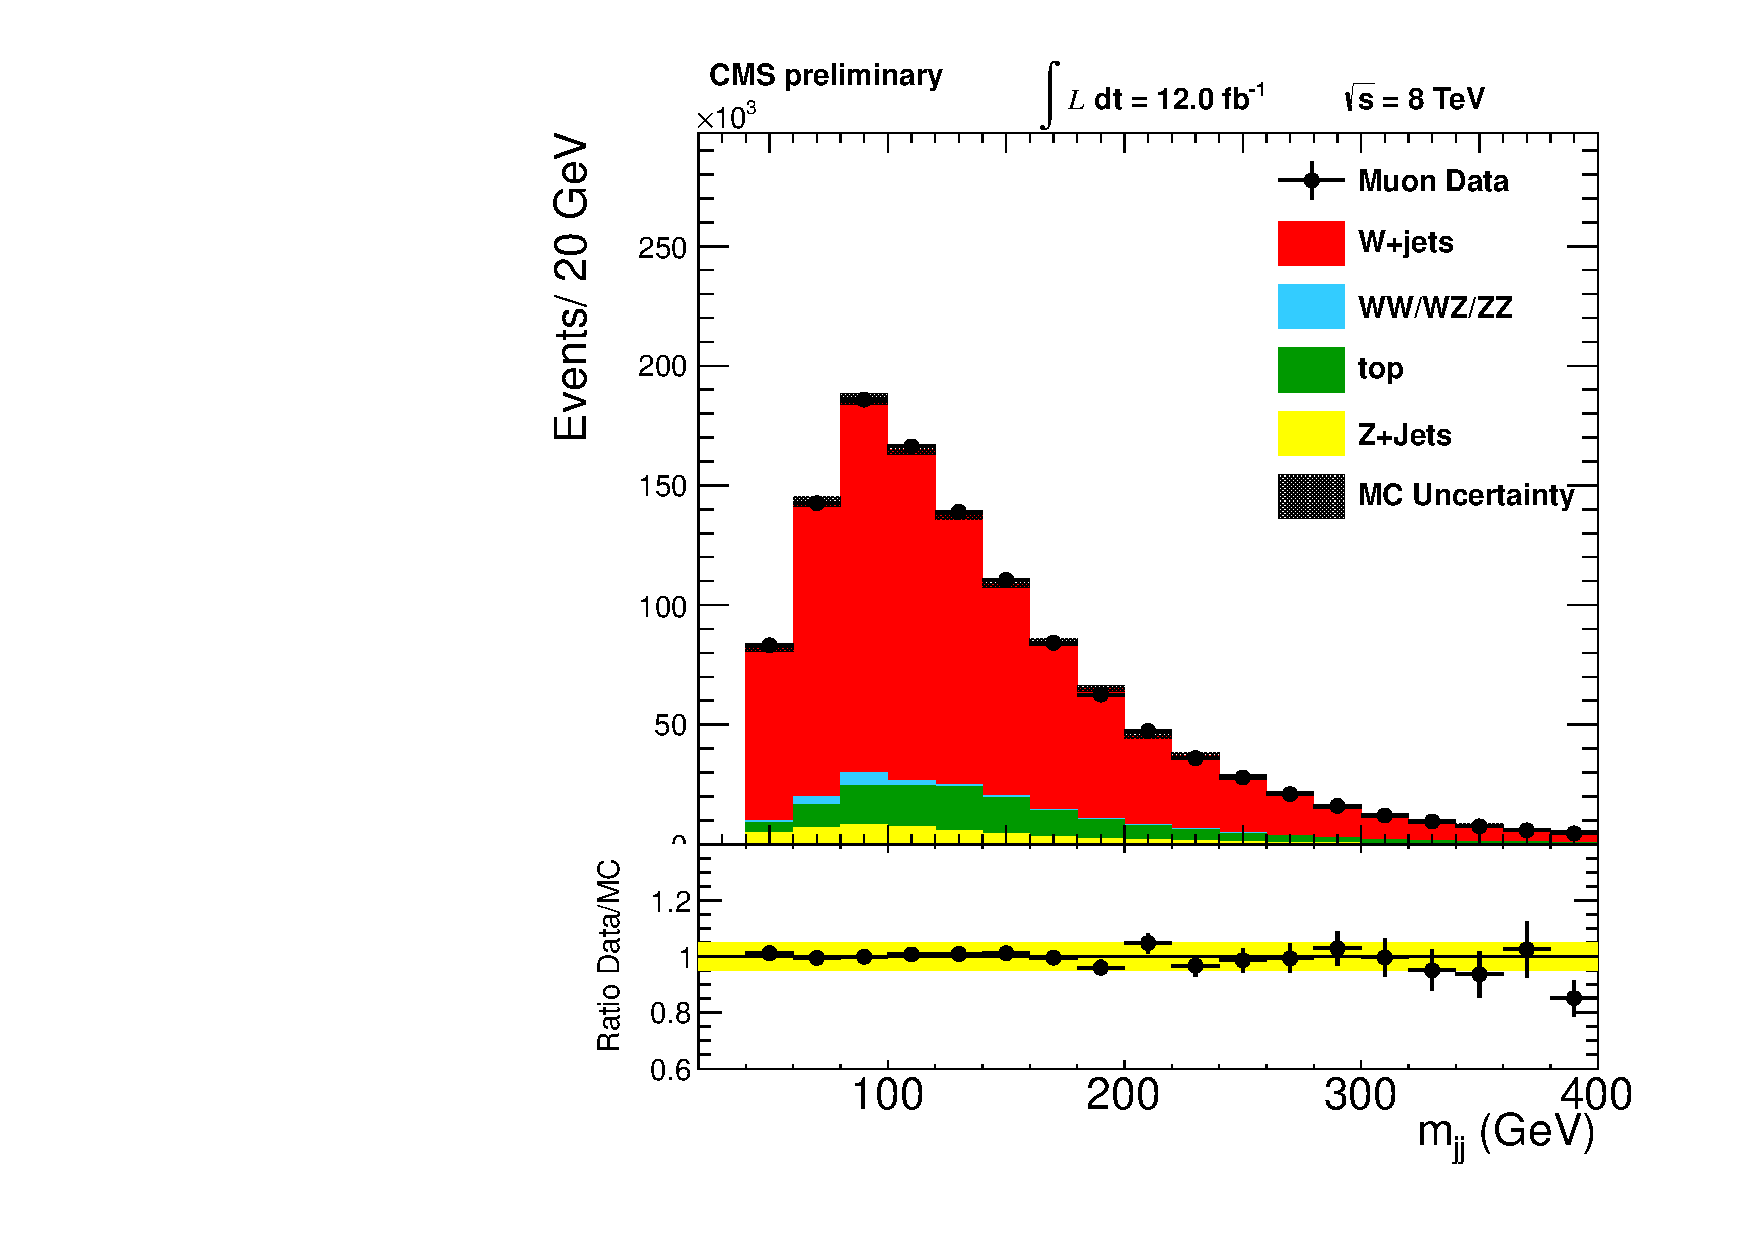
\includegraphics[width=0.45\textwidth]{plots/mu_mjj.pdf}
  }   
  \subfigure[]{
  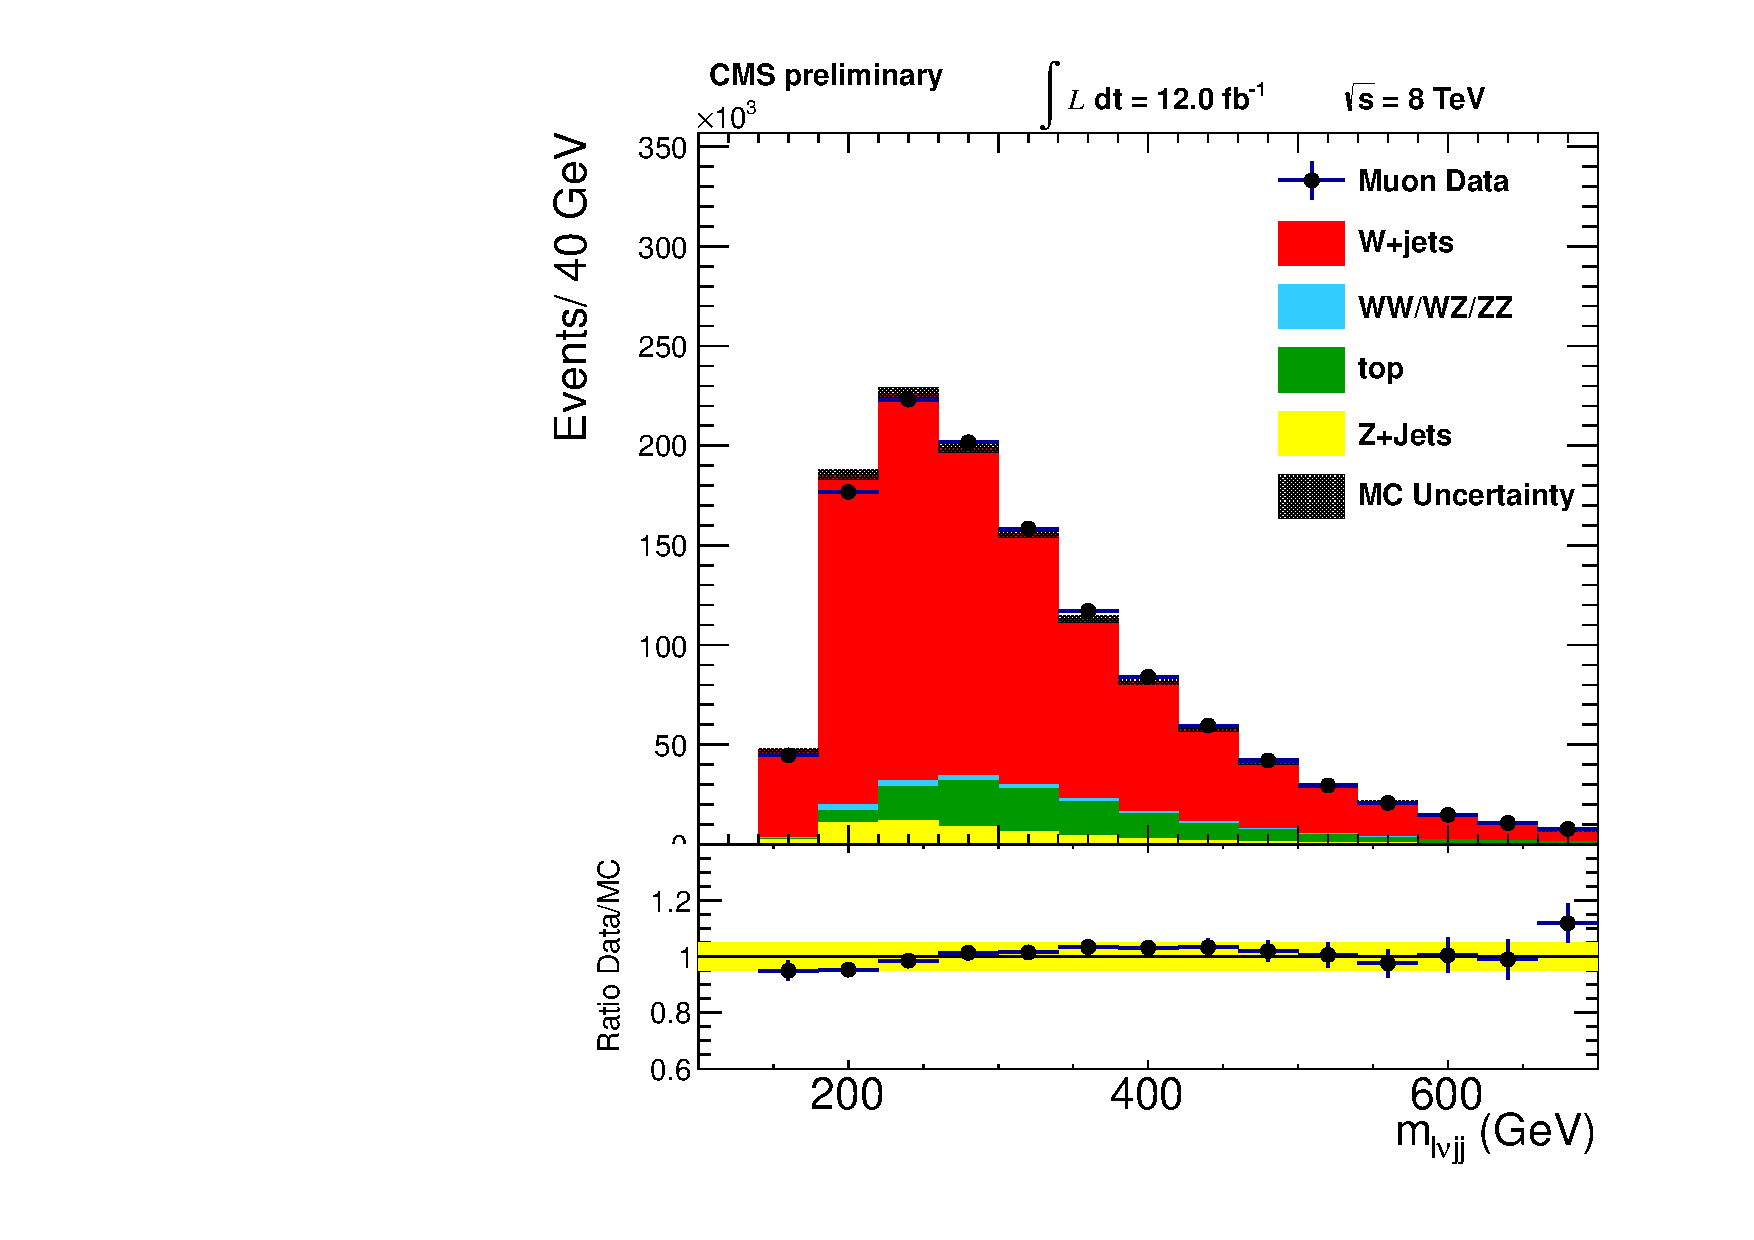
\includegraphics[width=0.45\textwidth]{plots/mu_mlvjj.pdf}
  }   
  \caption{The invariant mass of the dijet system ($m_{jj}$) and of
   the four-body system
  ($m_{\ell{}\nu{}jj}$) after the physics object selection but 
  before optimization, for the case of muons plus 2-jets sample. 
  While the W+jets simulation describes $m_{jj}$ distribution 
  in data well, the agreement in $m_{\ell{}\nu{}jj}$ is less good, 
  hence we estimate the dominant W+jets background contribution empirically using data sidebands.
  The error bars correspond to the statistical uncertainties. 
}
  \label{fig:massesPlots}
  \end{center}
\end{figure}
%%%%%%%%%%%%%%%%%

% ---- ---- ---- ---- ---- ---- ---- ---- ---- ---- ---- ---- ---- ---- ---- ---- ---- ---- ---- ---- ---- ----

\section{Selection optimization}
\label{sec:mva}
To exploit the differences in kinematics between signal and
background, a likelihood discriminant is constructed that incorporates
a set of variables that best distinguishes the Higgs signal from the
W+jets background. This approach improves the expected sensitivity to
a Higgs mass hypothesis across the entire mass range, but particularly
allows one to extract a limit below $M_H=250$~\GeVnn, where the background
is all the more dominant. These variables comprise five
angles between the Higgs decay products that fully describe the Higgs
production kinematics~\cite{Gao:2010qx}, the $\PT$ and rapidity of the
WW system, and the lepton charge.

\begin{figure}[t!]
  \begin{center}
    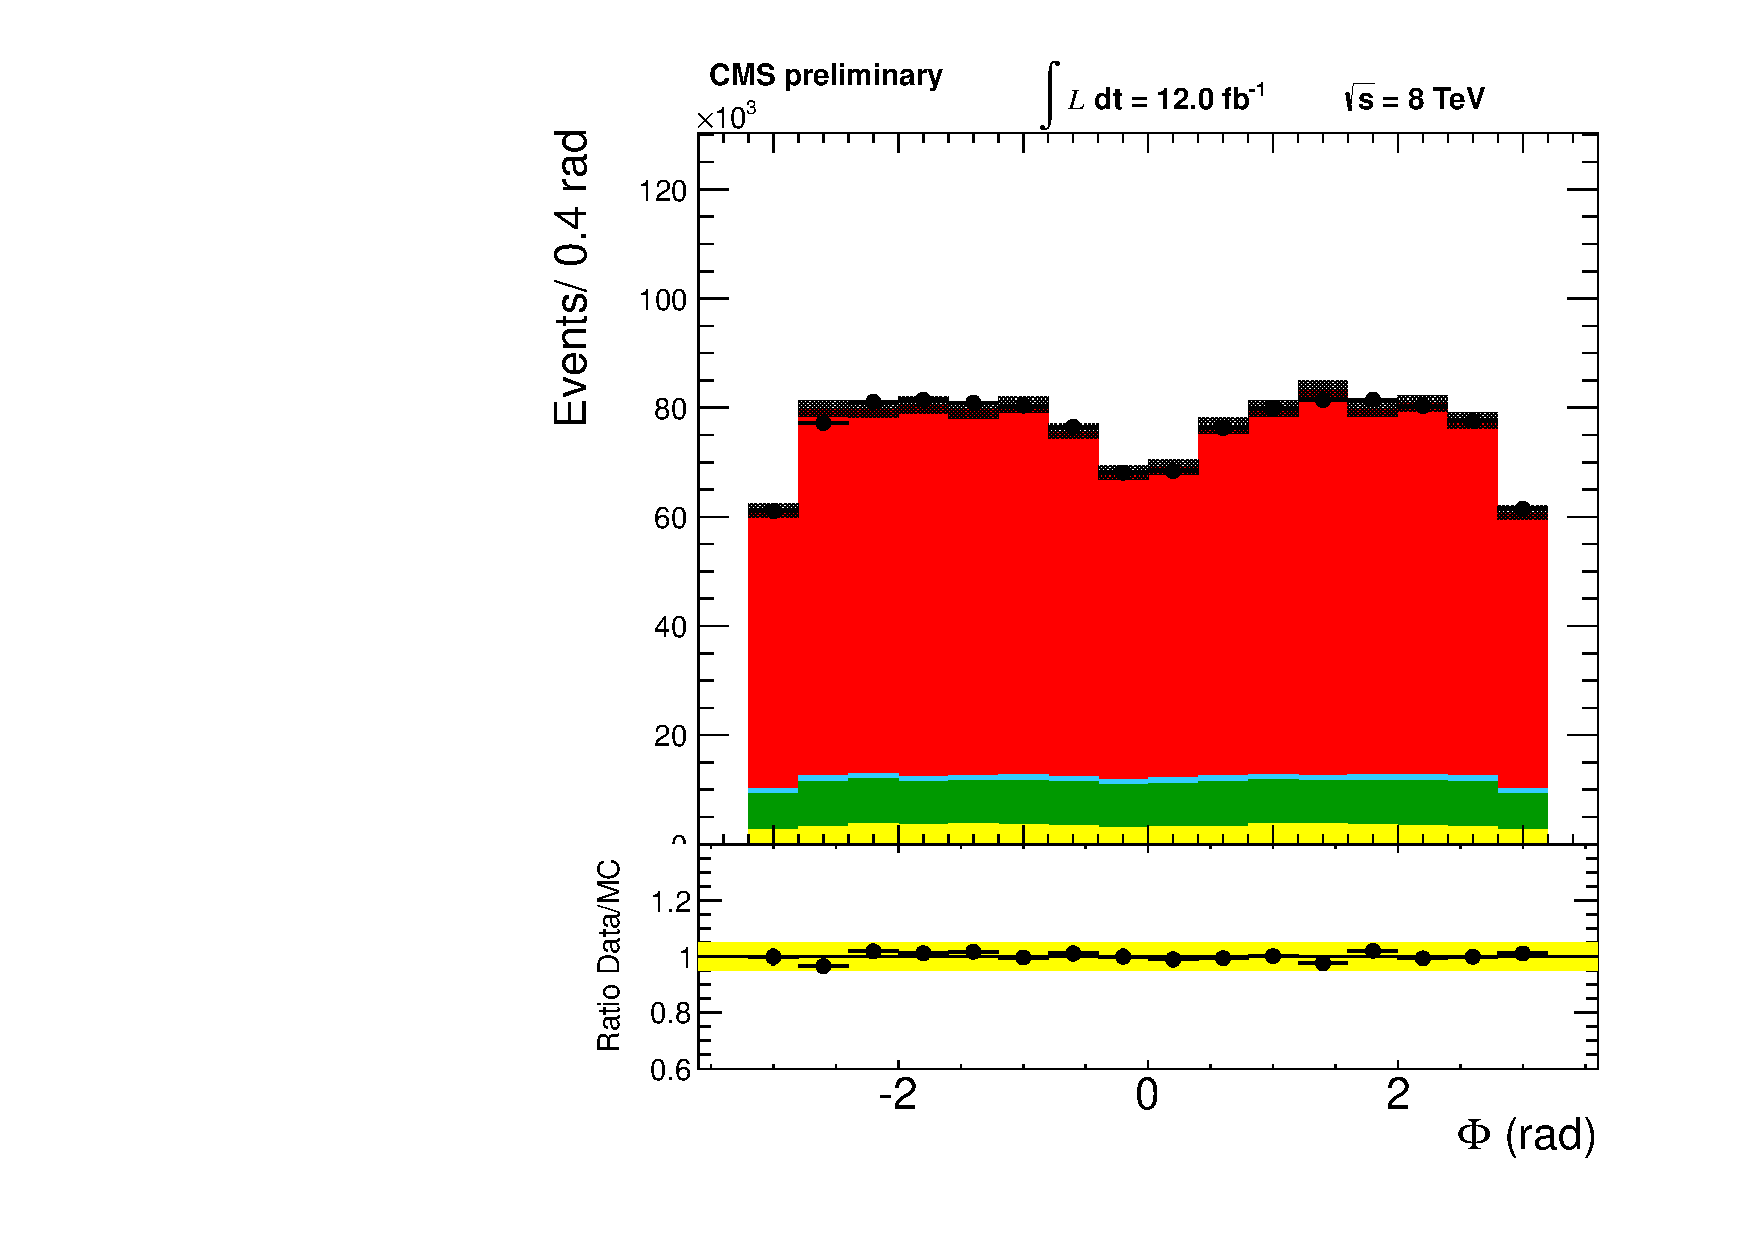
\includegraphics[width=0.3\linewidth]{plots/mu_phi.pdf}
    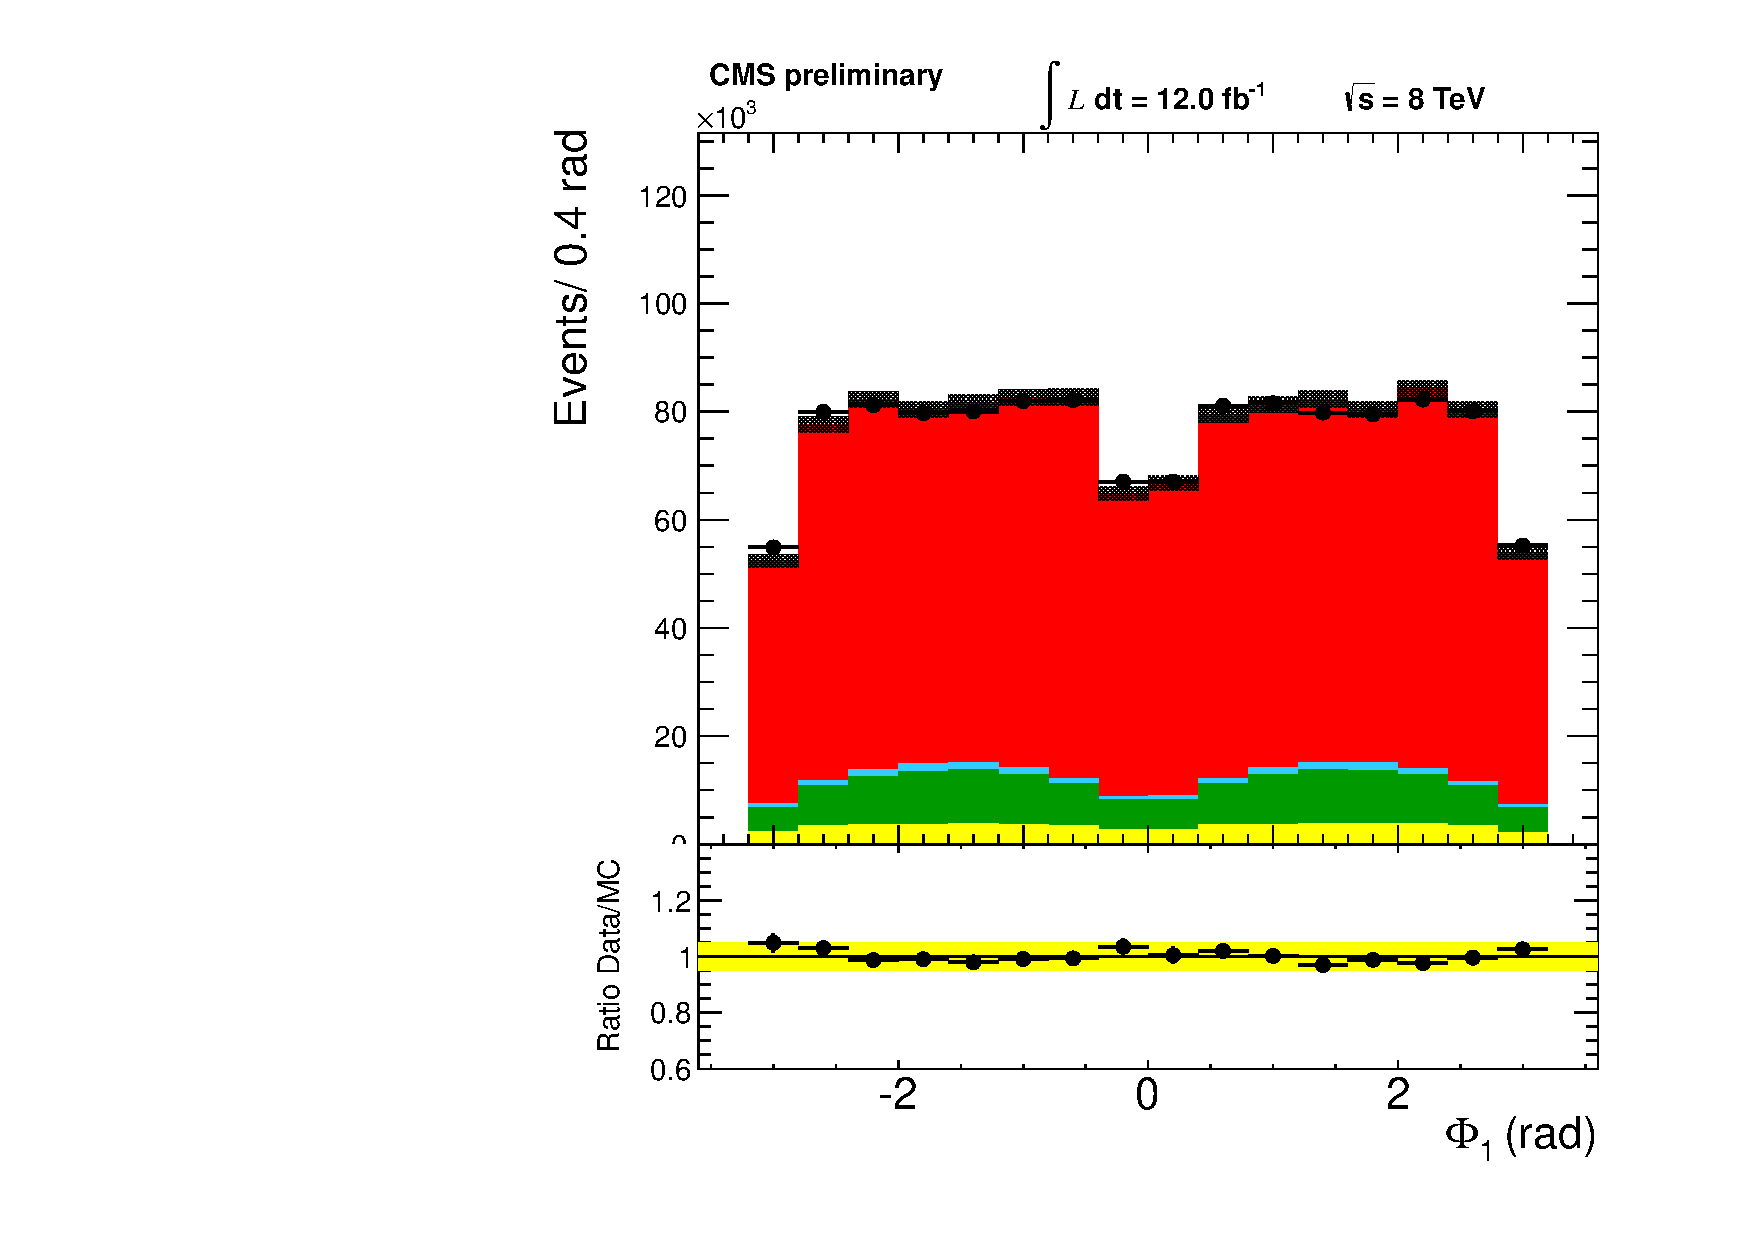
\includegraphics[width=0.3\linewidth]{plots/mu_phib.pdf}
    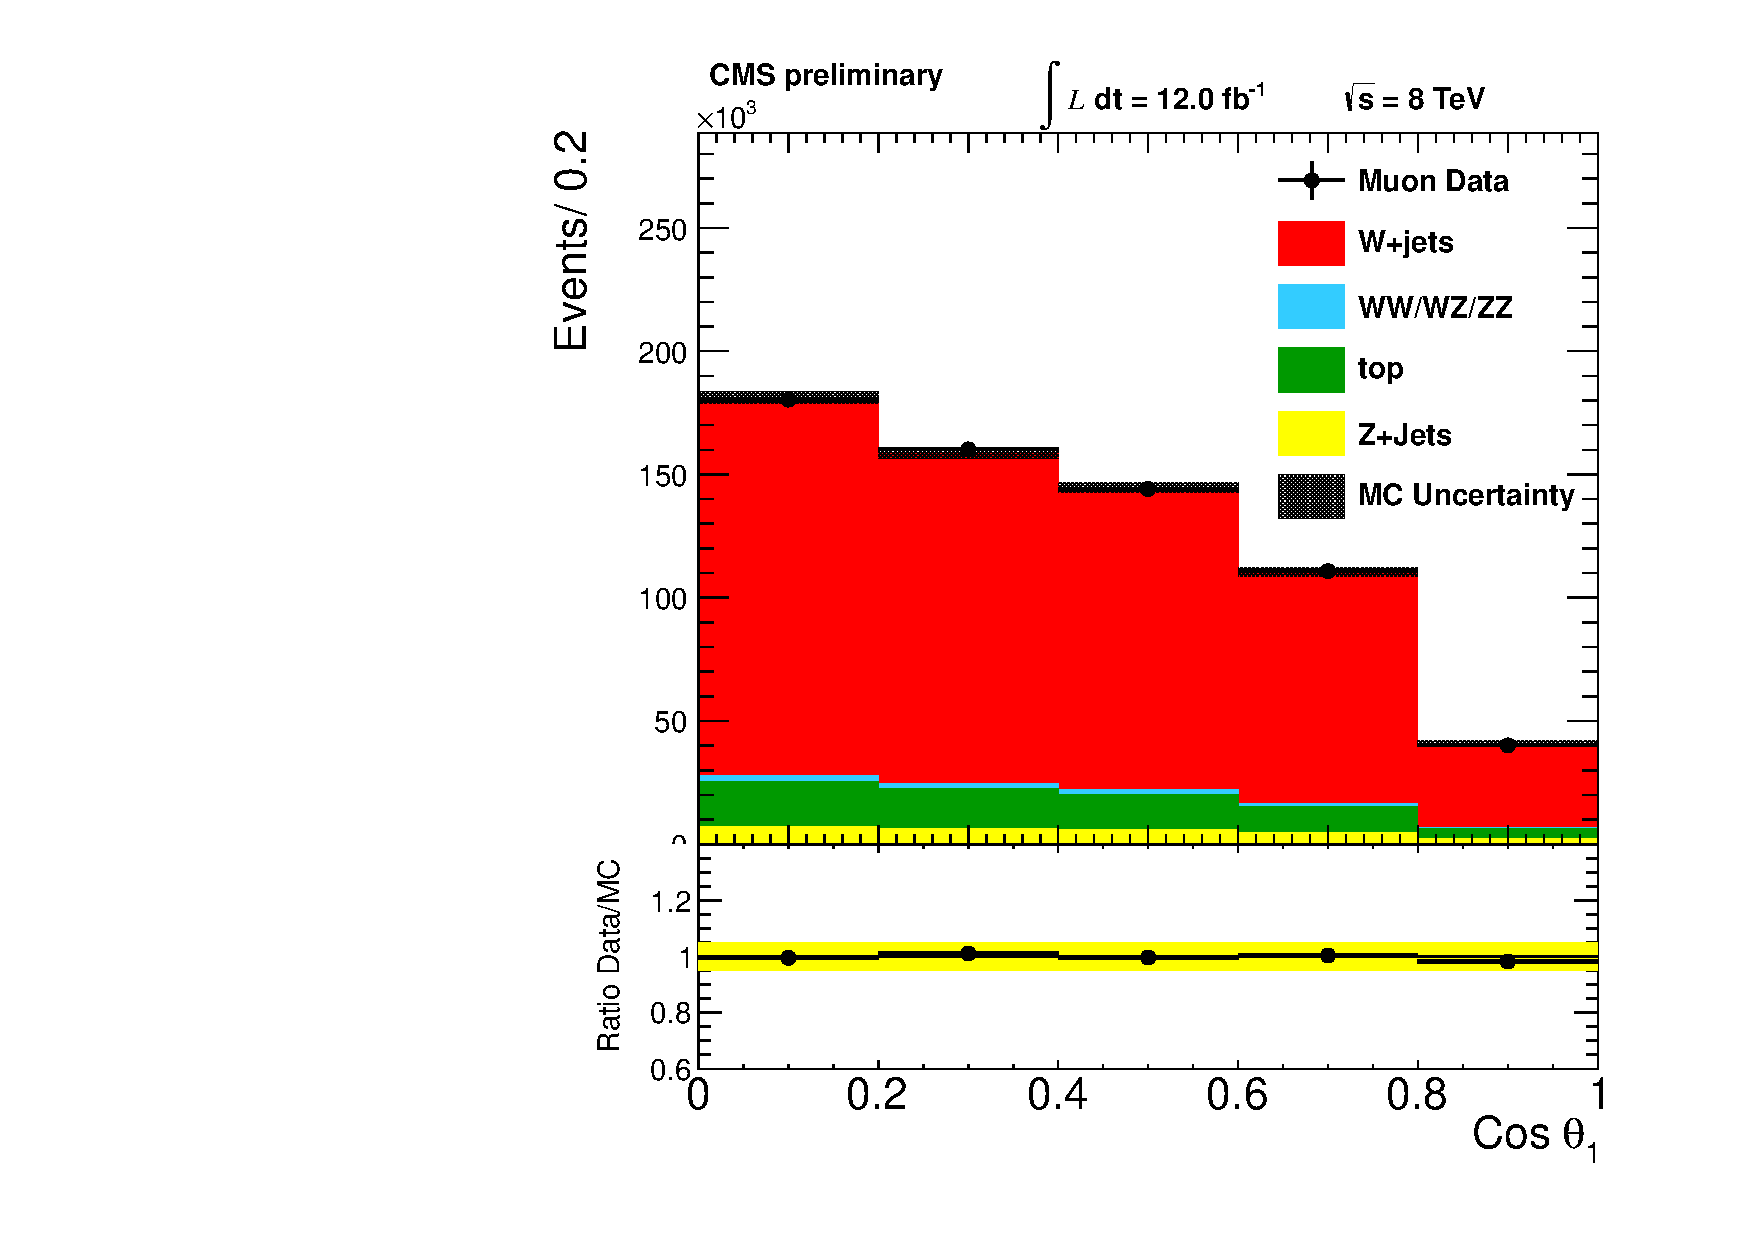
\includegraphics[width=0.3\linewidth]{plots/mu_ha.pdf}
    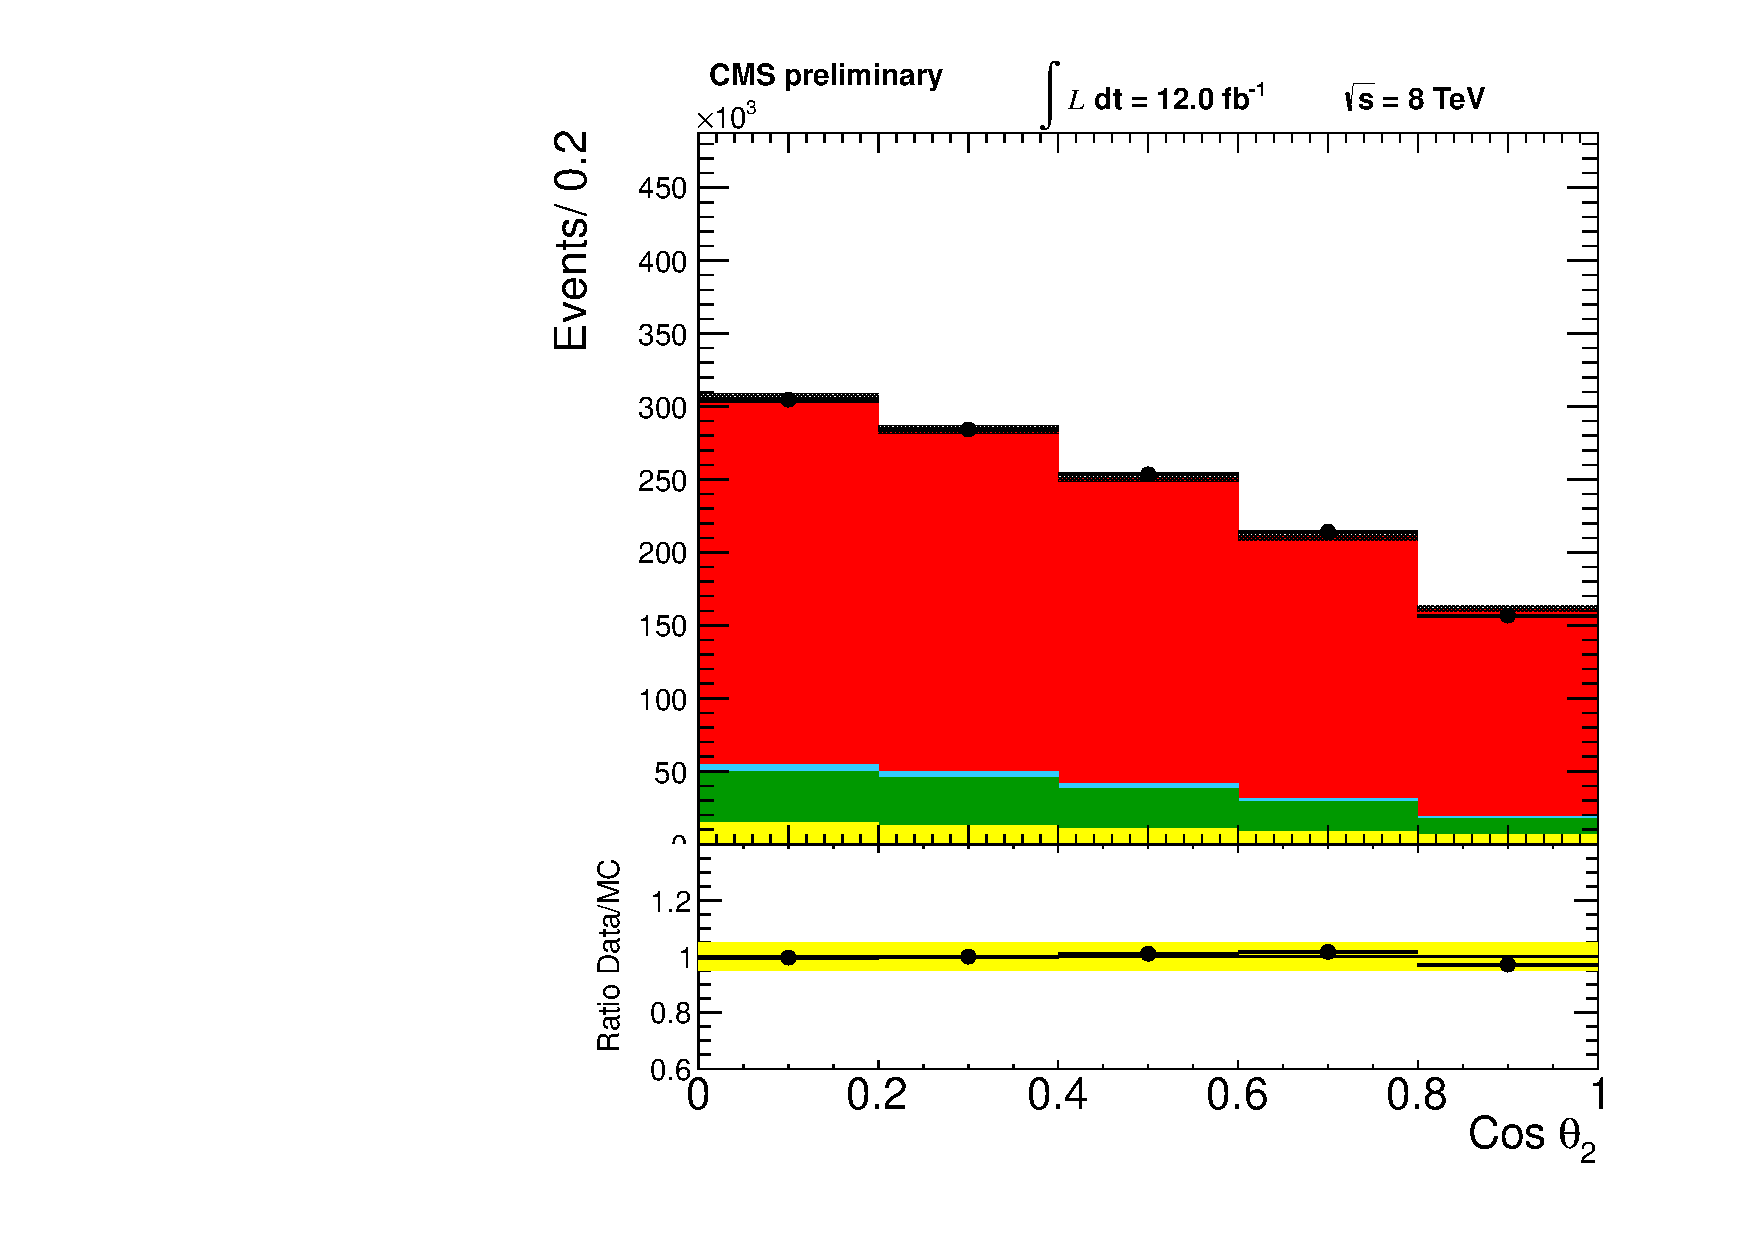
\includegraphics[width=0.3\linewidth]{plots/mu_hb.pdf}
    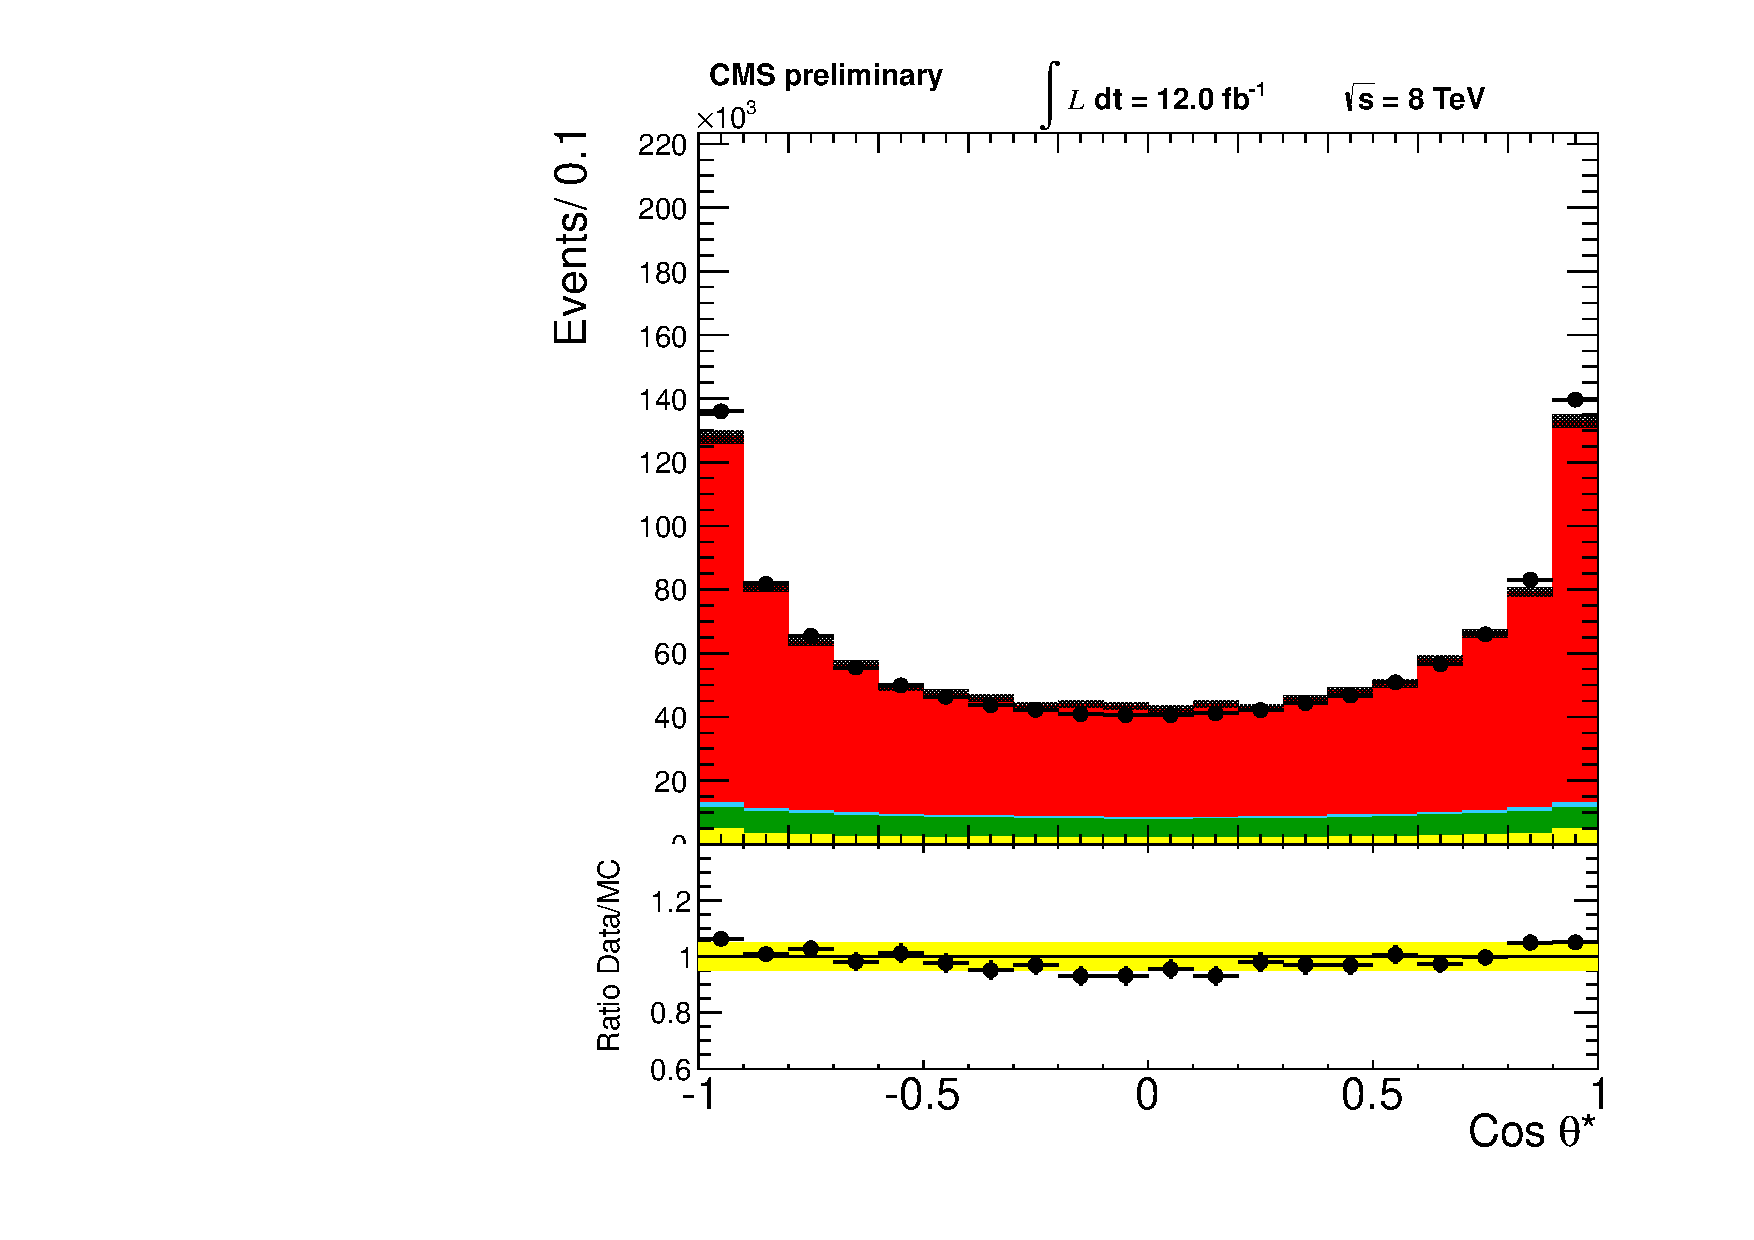
\includegraphics[width=0.3\linewidth]{plots/mu_hs.pdf}
    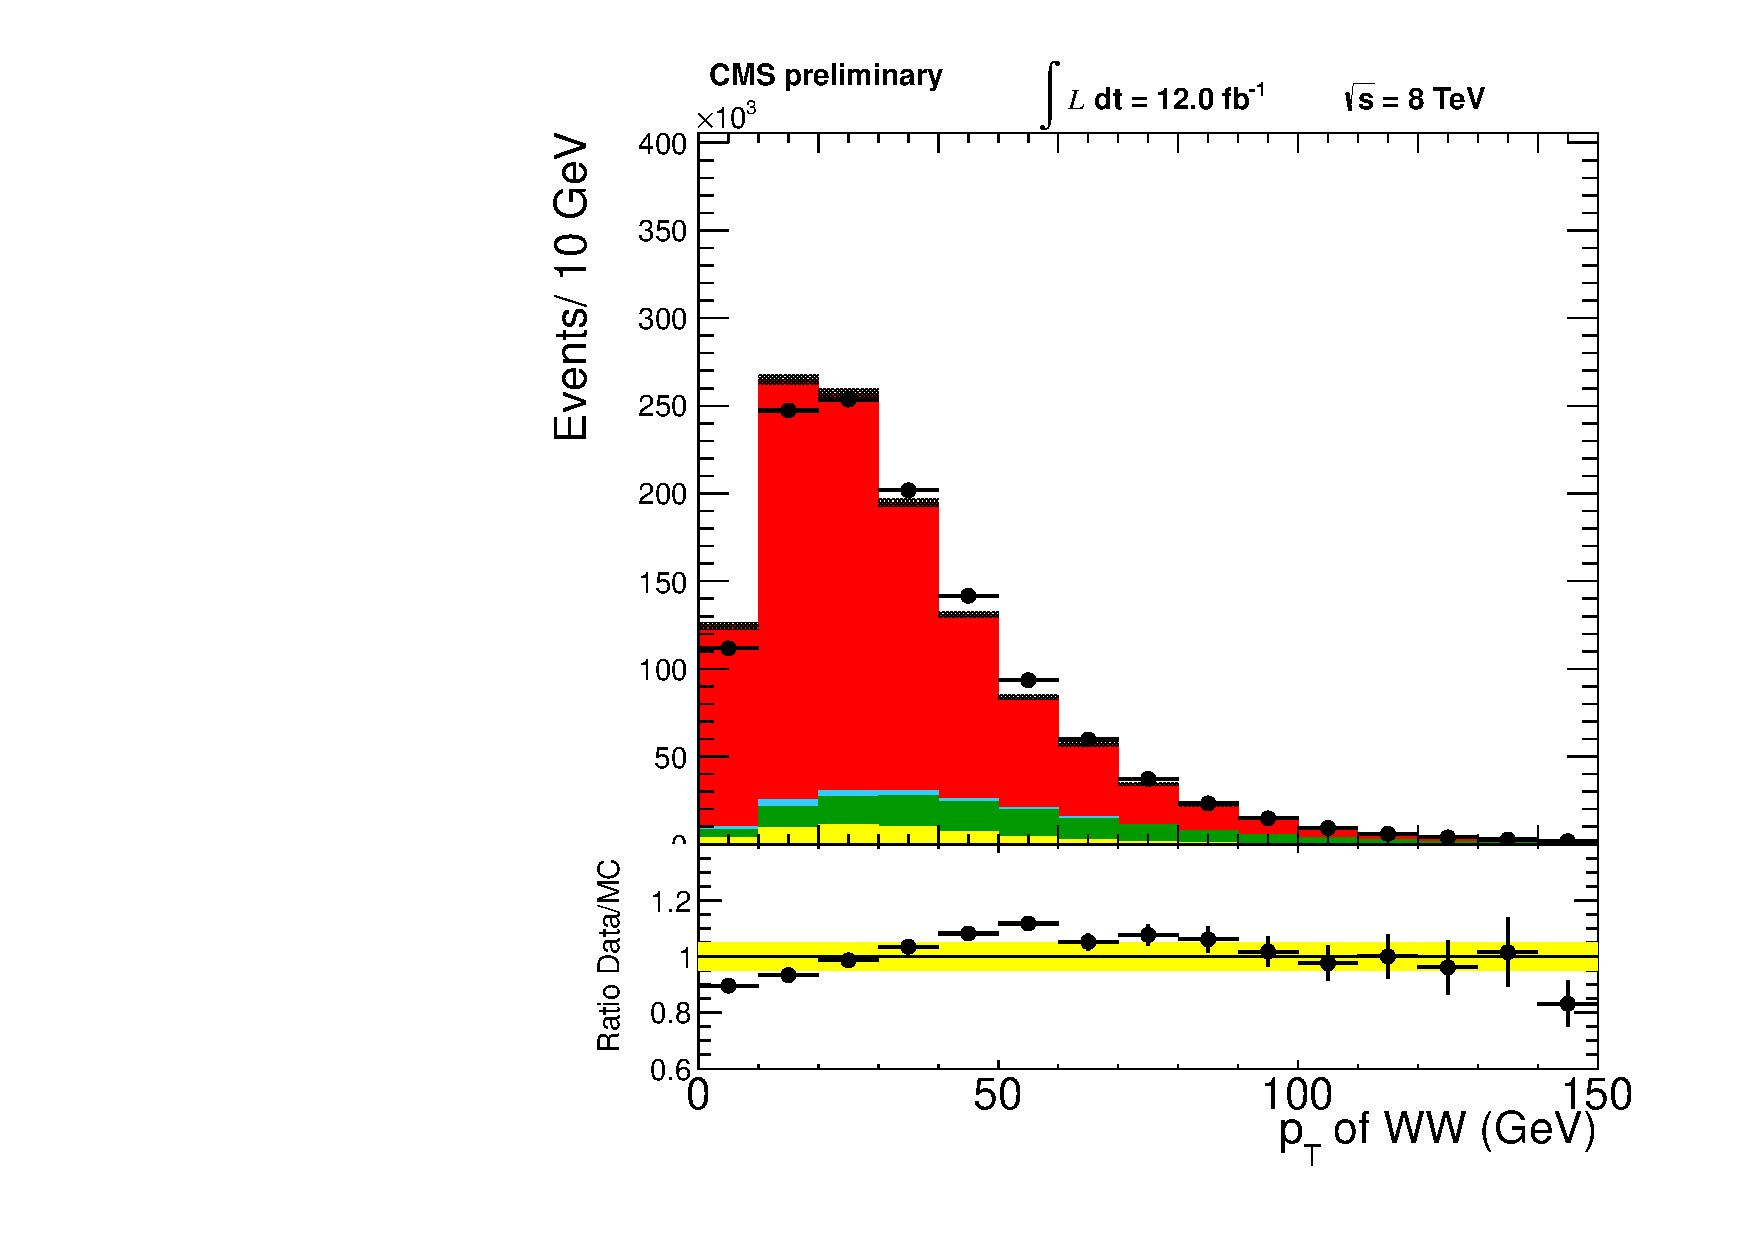
\includegraphics[width=0.3\linewidth]{plots/mu_ptlvjj.pdf}
    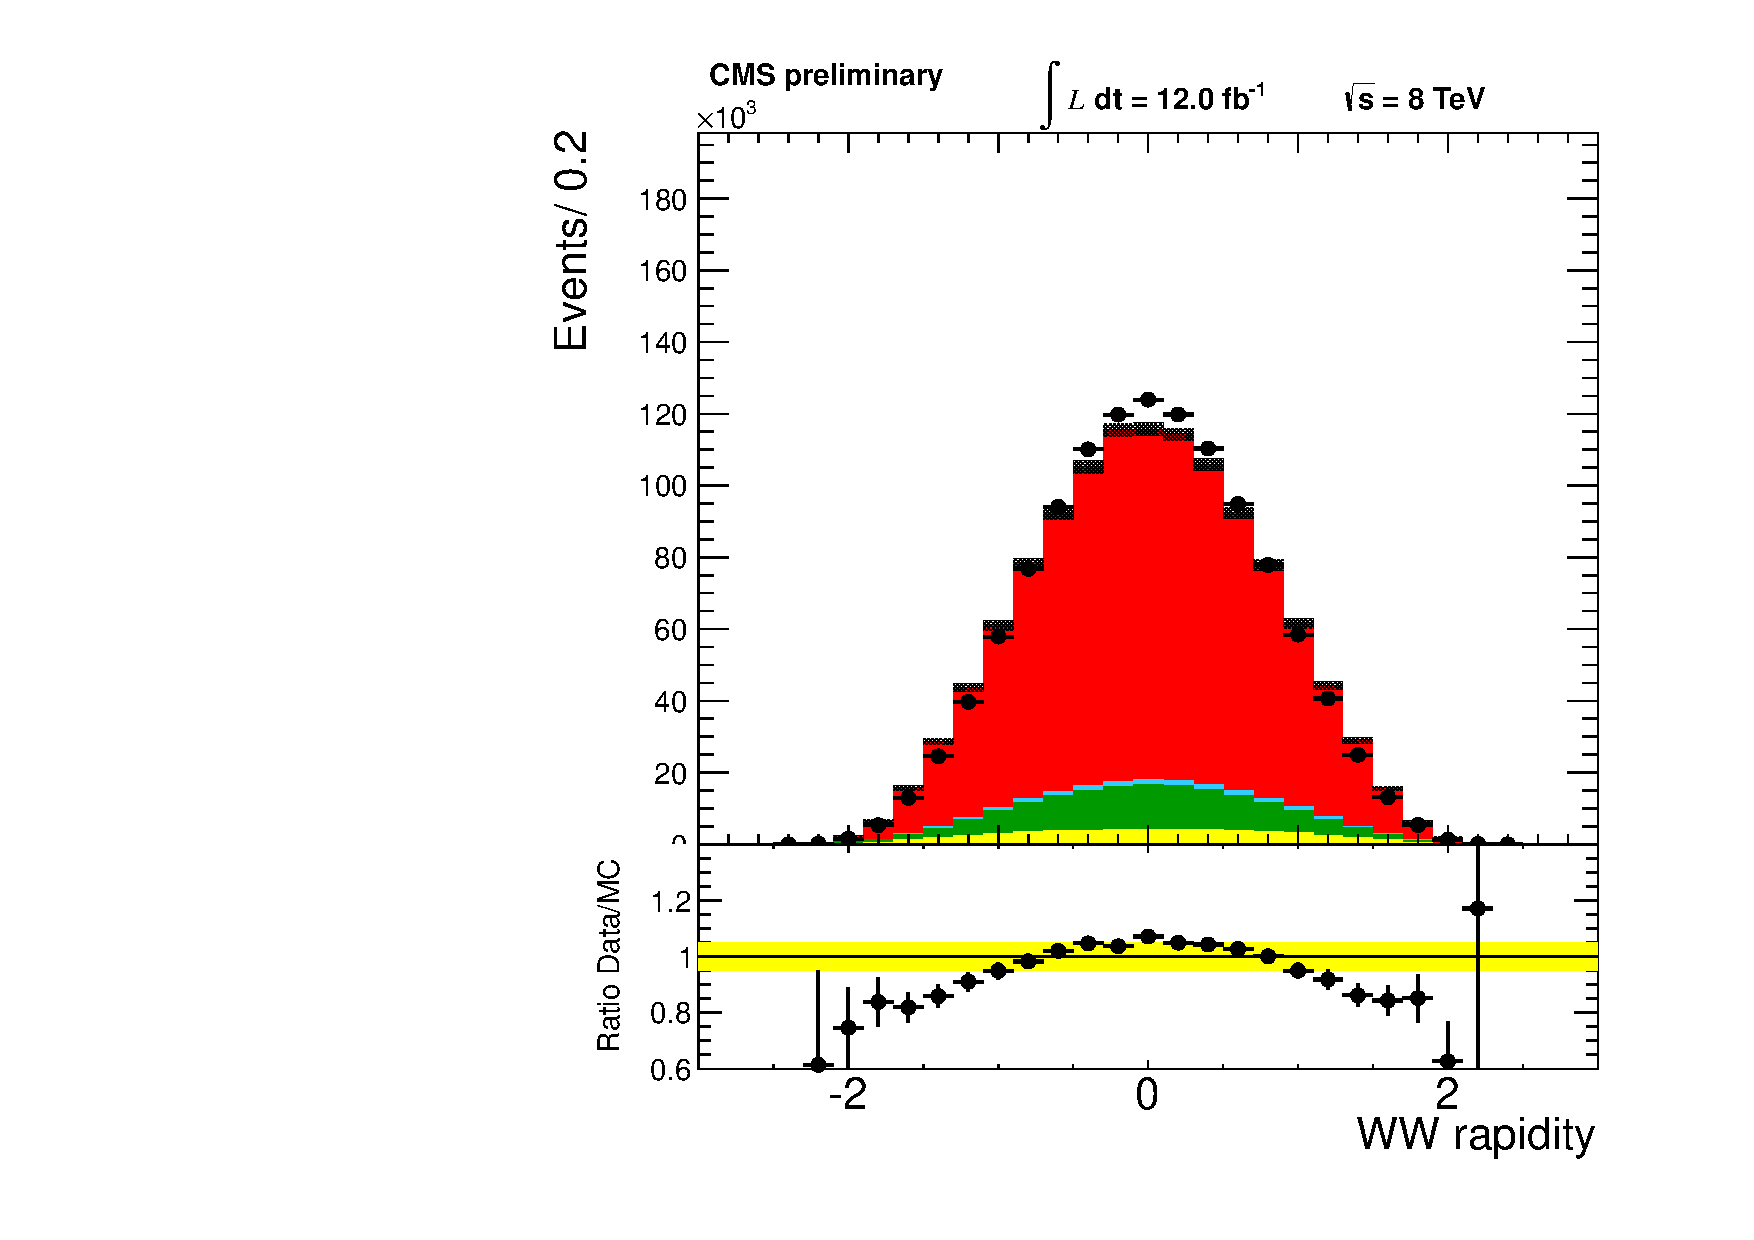
\includegraphics[width=0.3\linewidth]{plots/mu_etalvjj.pdf}
    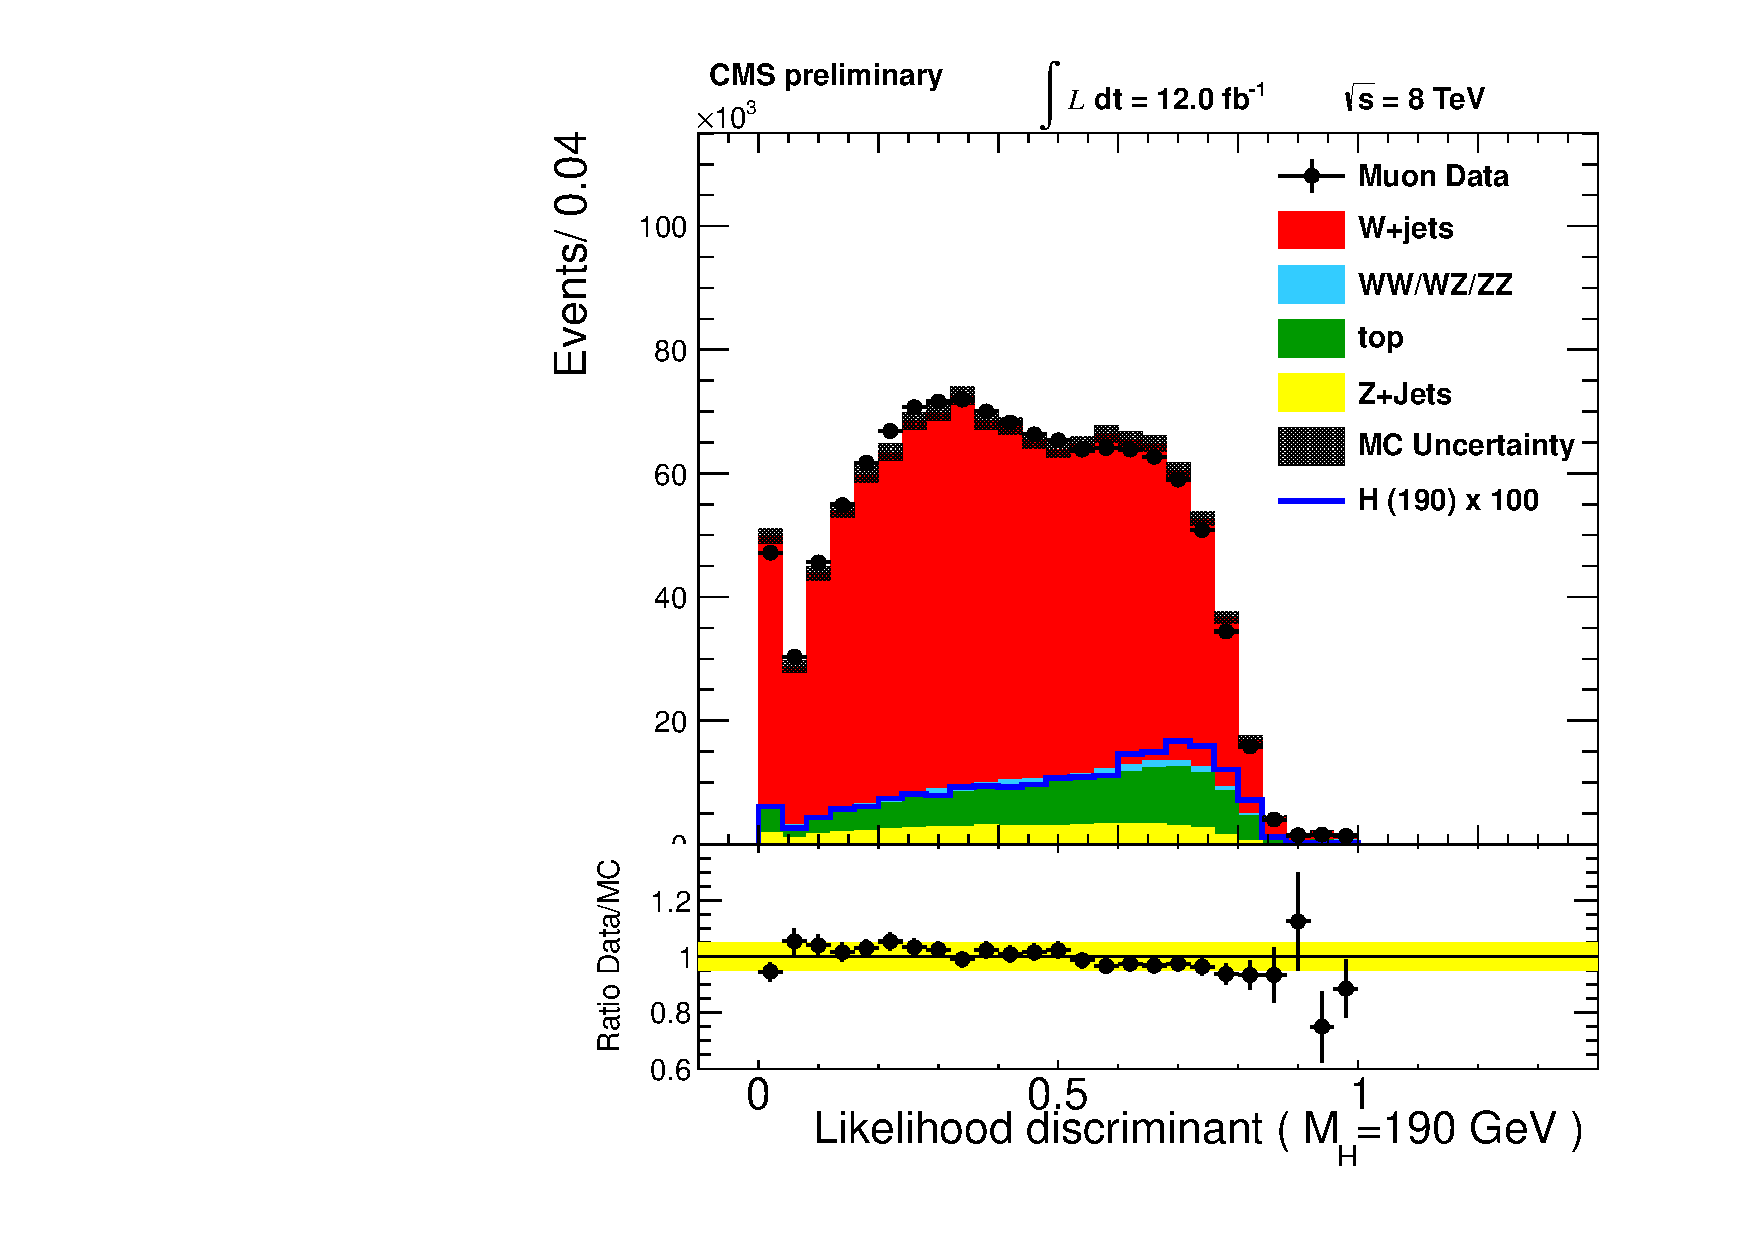
\includegraphics[width=0.3\linewidth]{plots/mu_mva2j190.pdf}
    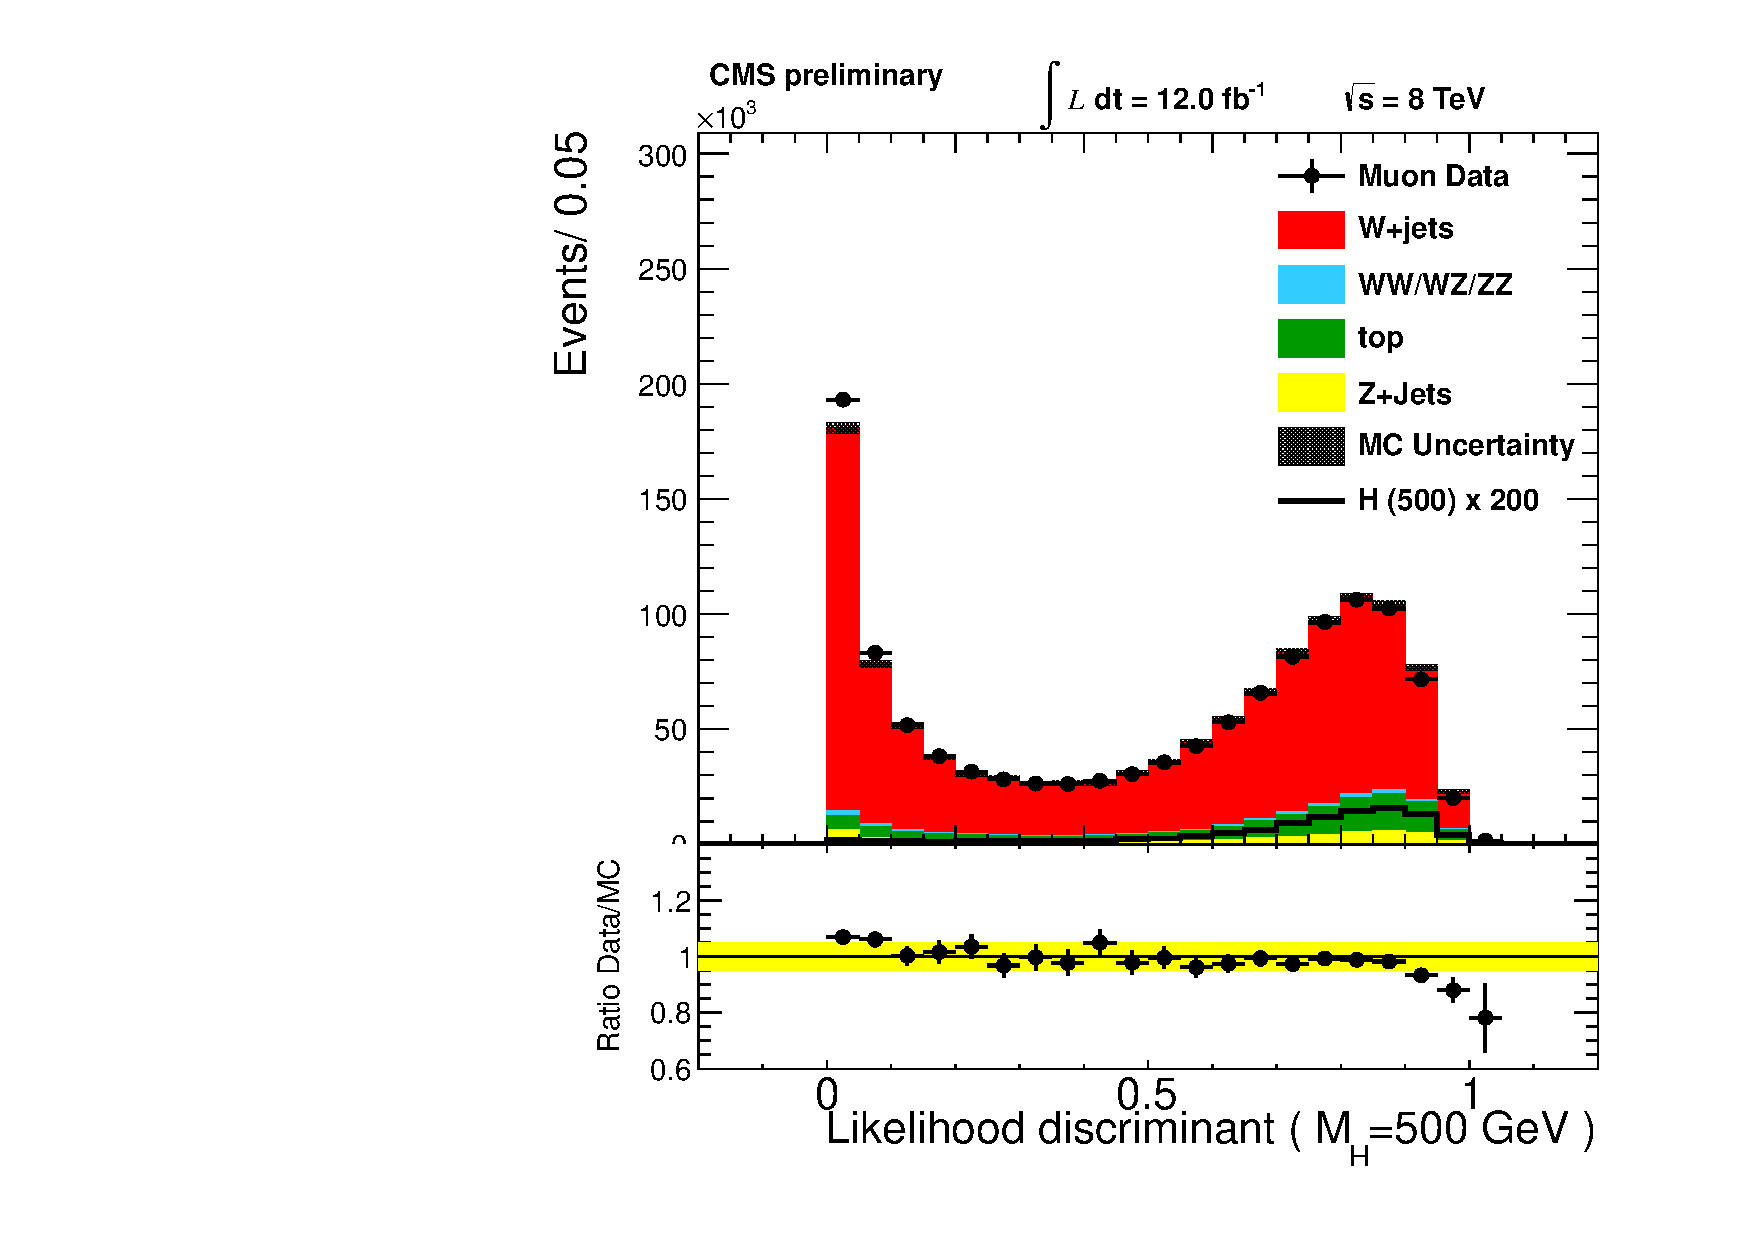
\includegraphics[width=0.3\linewidth]{plots/mu_mva2j500.pdf}
  \caption{The variables used as input for the likelihood discriminant. 
  From left to right, and from top to bottom: 
  $\Phi$, $\Phi_1$, $\theta_1$, $\theta_2$, $\theta^*$, $\PT$(WW), 
  and rapidity of the WW system. These variables are defined in 
  Ref.~\cite{HIG-11-027}. 
  Also shown in addition are the likelihood discriminants for the muon 
  plus 2-jets channel with selections optimized for Higgs mass 
  hypotheses of 190\GeVnn and 500\GeVnn. 
  The error bars correspond to the statistical uncertainties. 
  }
  \label{fig:mvaPlots}
  \end{center}
\end{figure}

The likelihood discriminant is optimized with dedicated simulation 
samples for 12 Higgs mass hypotheses (170, 180, 190, 200, 250, 300, 350, 
400, 450, 500, 550, 600) \GeVnn, for each
lepton flavor (e, $\mu$) and for each jet multiplicity (2 jets, 3 jets)
independently. 
In this way, 48 different optimizations are obtained. 
For each of them, events are retained if they survive a simple 
selection on the likelihood discriminant, chosen on the basis of the 
expected limit for the Higgs extraction as the figure of merit. 
Figure~\ref{fig:mvaPlots} shows the distribution of the 
discriminating variables for muons at the preselection level.

% ---- ---- ---- ---- ---- ---- ---- ---- ---- ---- ---- ---- ---- ---- 

\section{Background yields} %%% for the likelihood analysis}
\label{sec:mjjfit}

The background normalization in the signal region is extracted, for
each Higgs mass hypotheses independently, with an unbinned maximum likelihood
fit to the dijet invariant mass distribution $m_{jj}$ of the two
leading jets. The signal region corresponding to the W mass window,
$65\GeVnn < m_{jj} < 95\GeVnn$, is excluded from the fit.  The W+jets
shape is taken from simulation for Higgs mass hypotheses at or below
200\GeVnn. For higher masses the simulation doesn't have enough
events, so we describe the shape analytically using an exponential fit
function.  The overall normalization of the W+jets component is
allowed to vary in the fit.  The electroweak diboson, \ttbar, single
top, and Drell-Yan+jets shapes are based on simulation and their
normalization are constrained to the theoretical predictions, within
the corresponding uncertainties.  In case of diboson backgrounds, both
WW and WZ normalizations are constrained to the next-to-leading order
predictions within the uncertainties.  The multi-jet background shape
is derived from data by relaxing lepton isolation and identification
requirements. Its contribution to the total number of events is evaluated
from a separate two-component likelihood fit to the W transverse mass
distribution, and constrained in the $m_{jj}$ fit according to this
fraction within uncertainties.  Table~\ref{tab:mjjfit} summarizes the
determination of the shape and normalization for each contributing
process in the fit. Examples of the $m_{jj}$ fit are shown in
Figure~\ref{fig:mjj_mH350} for the muon channel, with selections
optimized for Higgs mass hypotheses 190\GeVnn, 300\GeVnn, and
500\GeVnn. The uncertainties in the normalization obtained from the
fit are propagated to the limit calculation as a systematic uncertainty.
The signal $m_{jj}$ distributions are shown in figure~\ref{fig:mjj_signals}
for varying Higgs mass hypotheses. 

\begin{table}[!ht]
 \begin{center}
  \begin{tabular}{lcl}
   \hline
   \hline
   Process        & Shape & External constraint on normalization \\
   \hline
   W+jets         & data/MC & Unconstrained \\
   Diboson       & MC      & Constrained: (NLO) $89.4\pb \pm 10\%$ \cite{MCFM} \\ 
   \ttbar         & MC      & Constrained: (approx. NNLO) $225\pb \pm 7\%$ \cite{Kidonakis:2010dk} \\
   single top     & MC      & Constrained: (approx. NNLO) $113\pb \pm 5\%$ \cite{Kidonakis:2010ux,Kidonakis:2010tc,Kidonakis:2011wy} \\
   Drell-Yan+jets & MC      & Constrained: (NNLO, $m_{\ell\ell}>50\GeV$) $3504\pb \pm 4.3\%$ \cite{Gavin:2010az}\\
   Multi-jet      & data    & Constrained: \MET fit in data $\pm$ 50\% (100\%) for electrons (muons) \\
   \hline
   \hline
  \end{tabular}
 \end{center}
 \caption{Determination of the $m_{jj}$ shape and normalization. External constraints are assumed
 to be Gaussian.}
 \label{tab:mjjfit} 
\end{table}

\begin{figure}[!t]
  \centering
  \subfigure[]{
  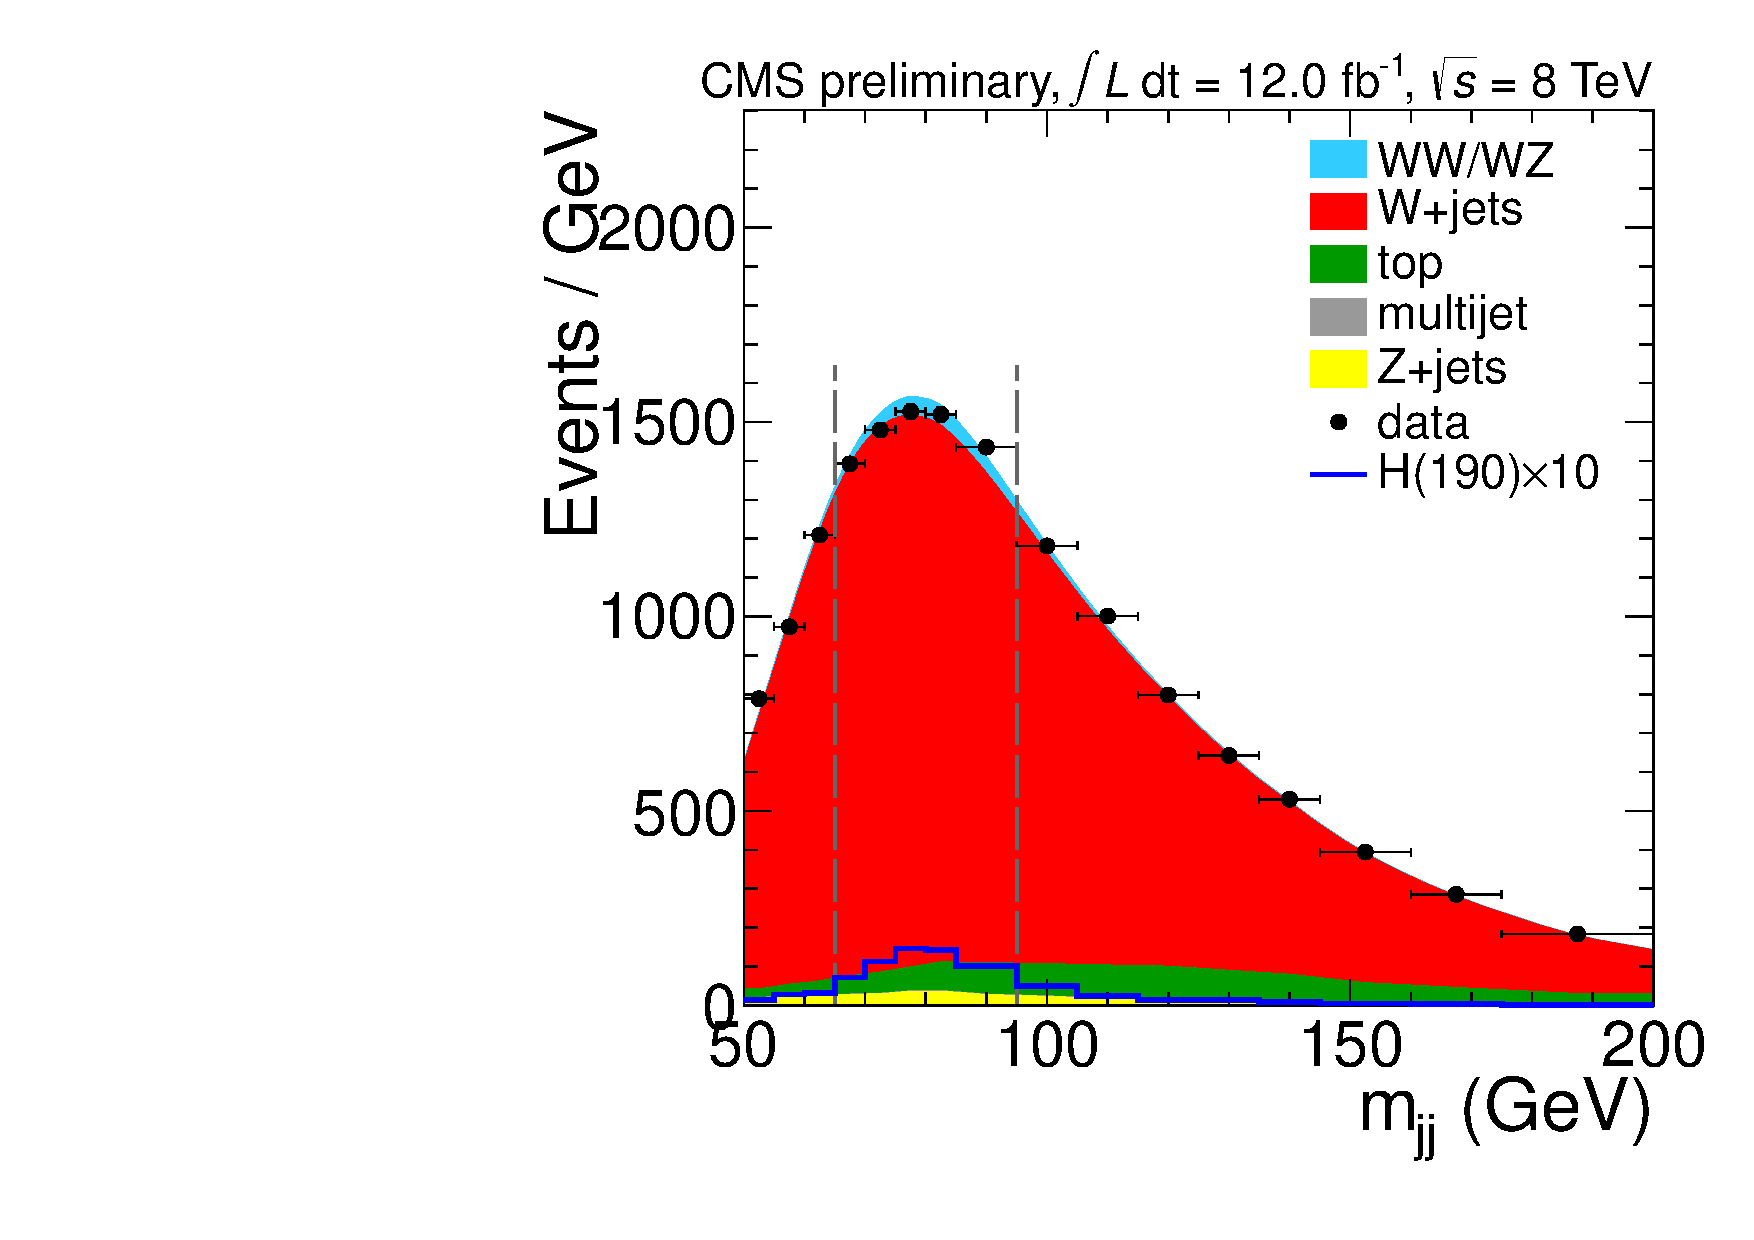
\includegraphics[width=0.32\textwidth]{plots/H190_Mjj_Muon_2jets_Stacked.pdf}
  }  
  \subfigure[]{ 
  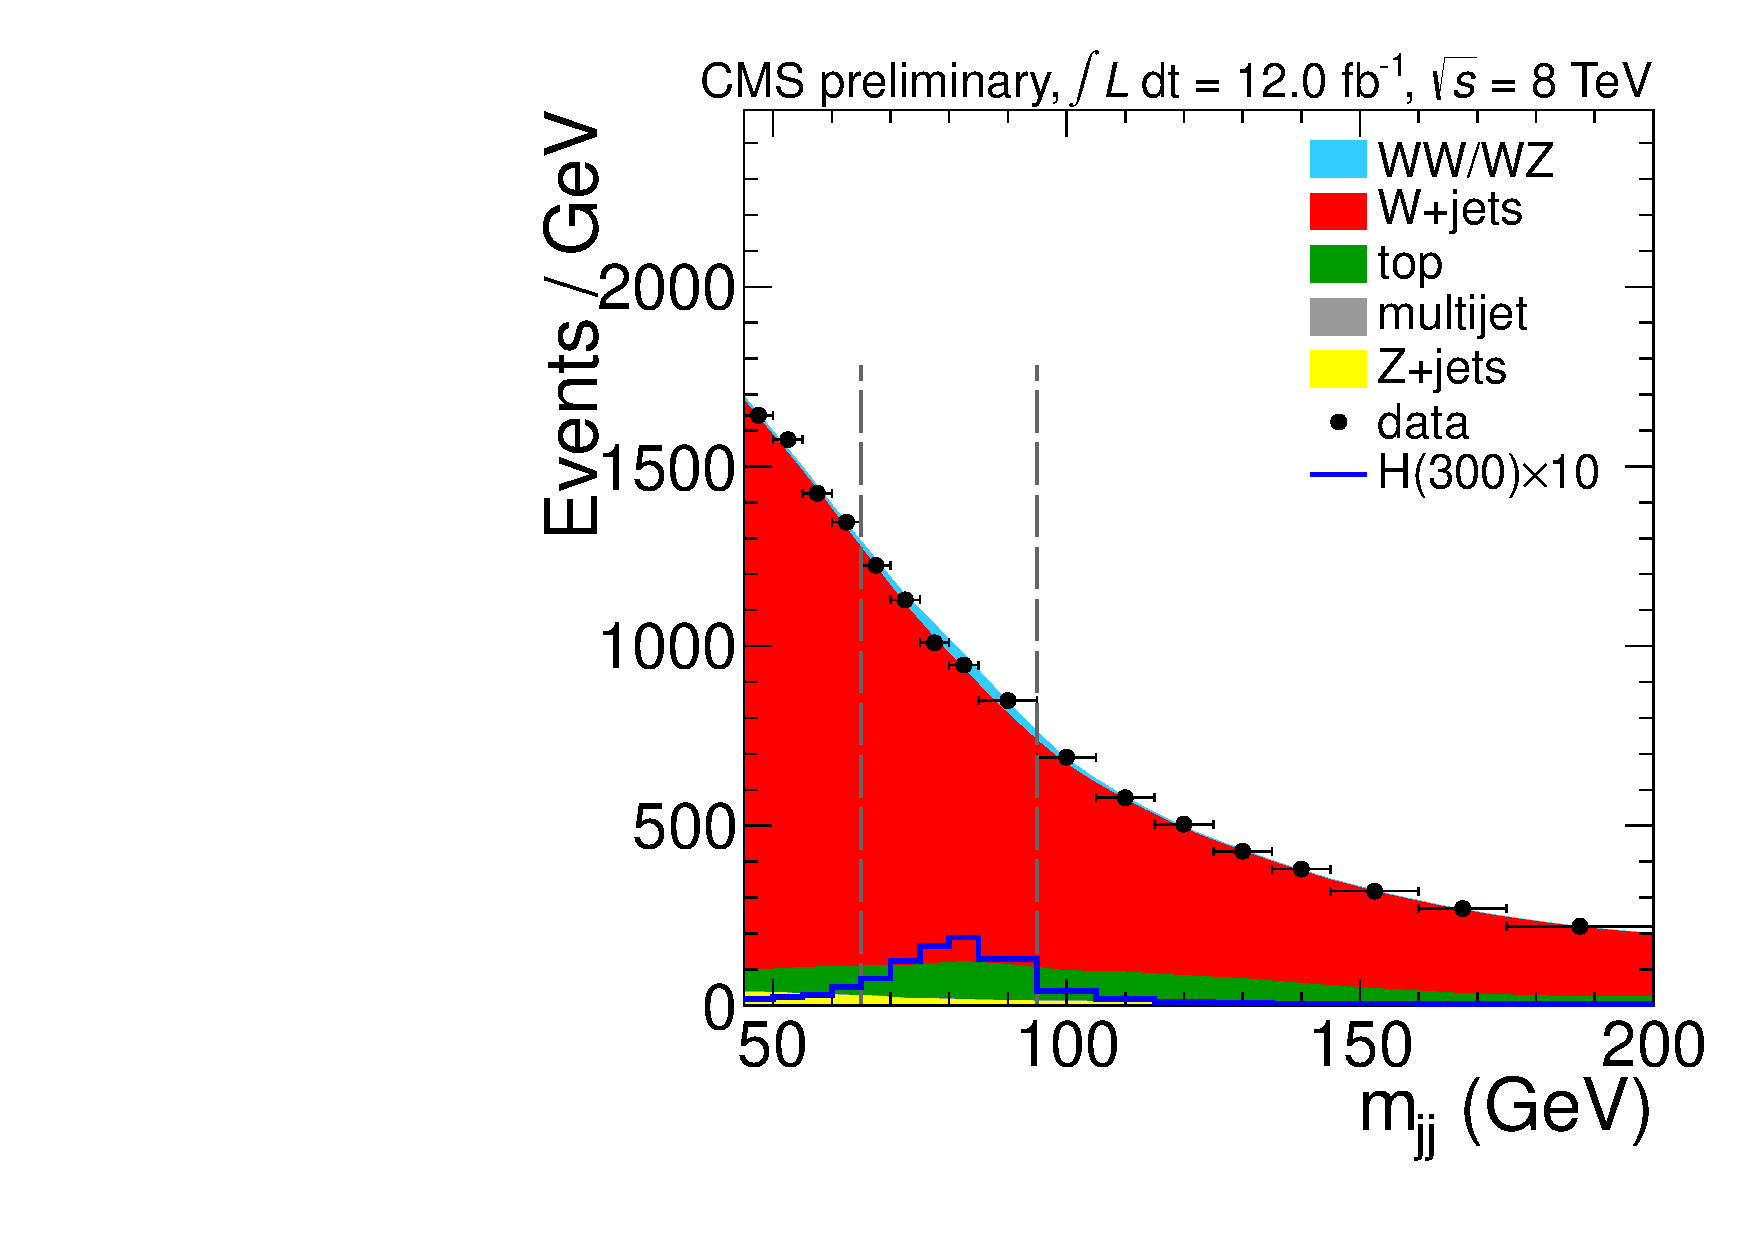
\includegraphics[width=0.32\textwidth]{plots/H300_Mjj_Muon_2jets_Stacked.pdf}
  }  
  \subfigure[]{ 
  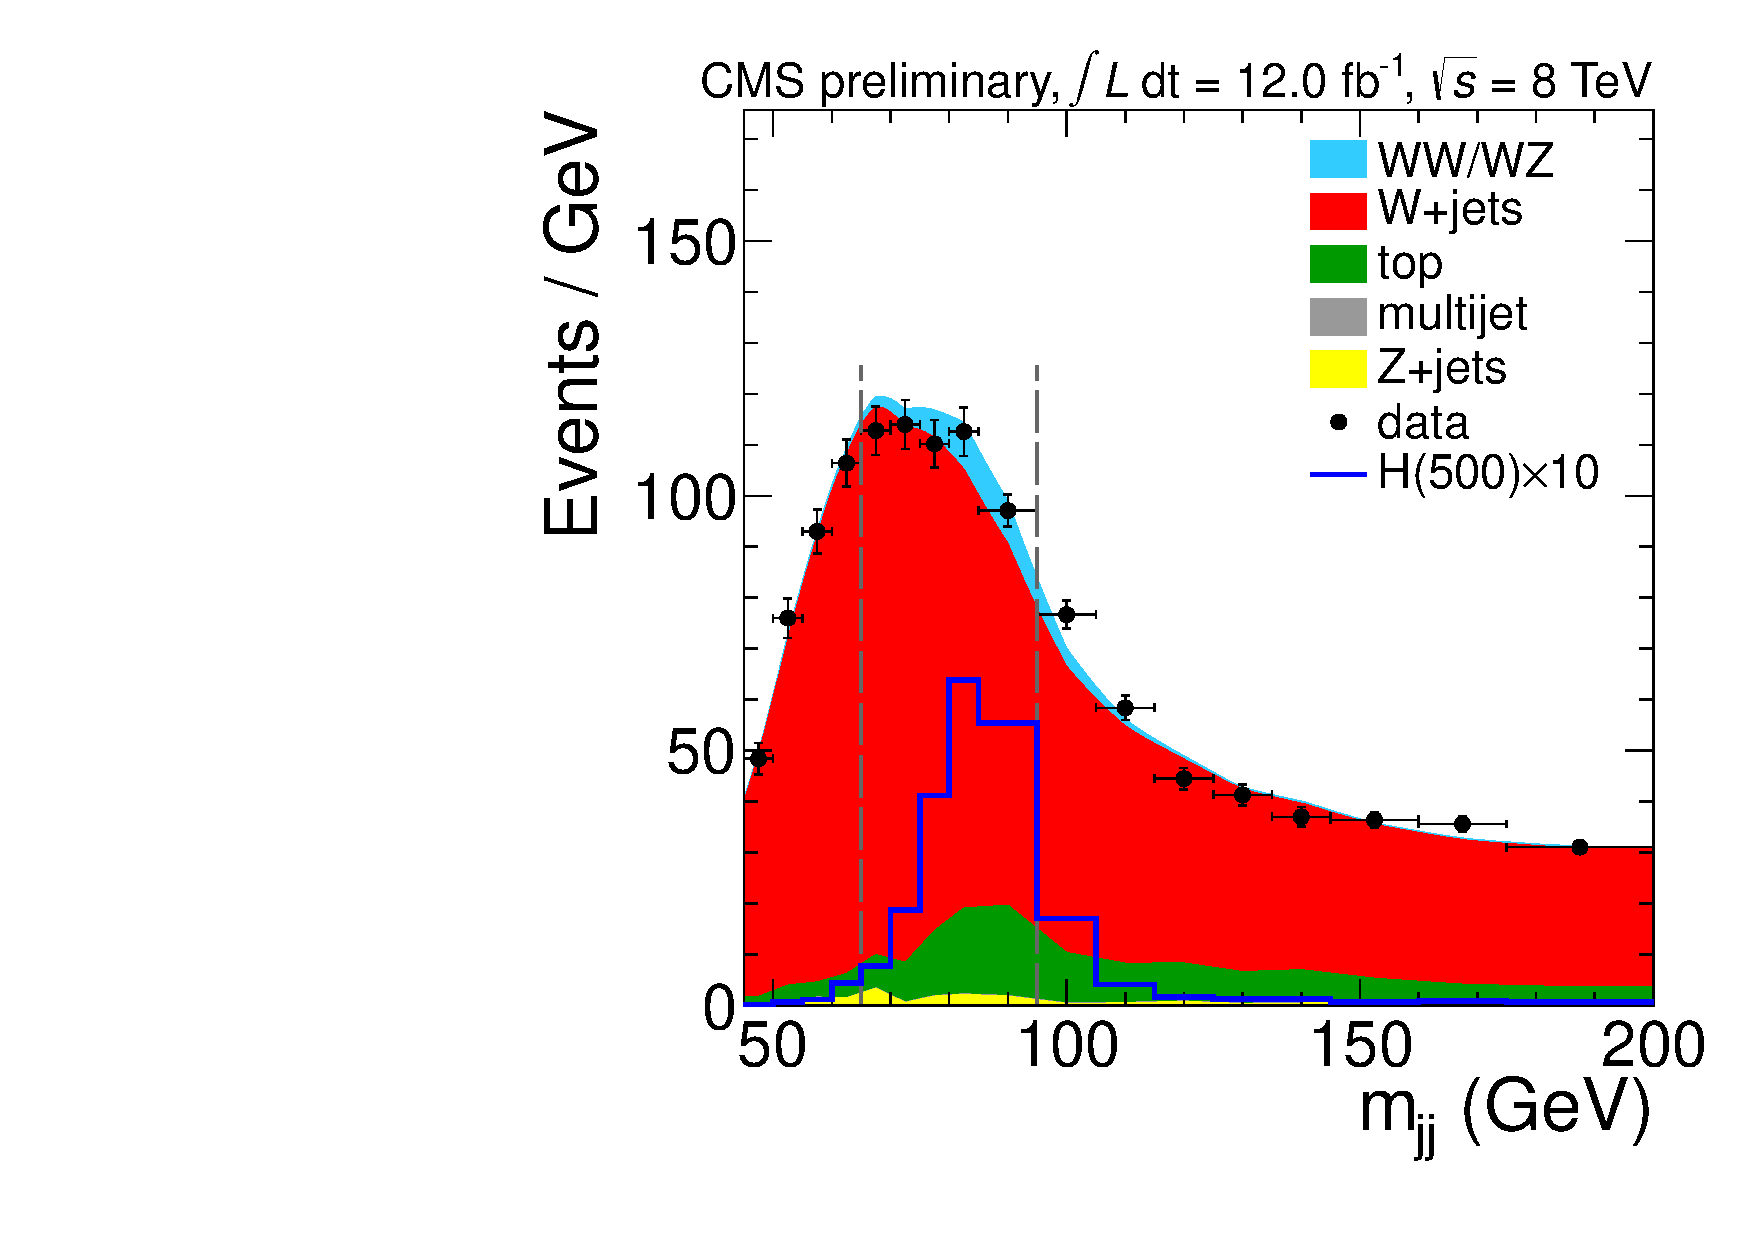
\includegraphics[width=0.32\textwidth]{plots/H500_Mjj_Muon_2jets_Stacked.pdf}
  }   
  \caption{\label{fig:mjj_mH350} The dijet invariant mass 
  distribution with the fit projections, for the muon plus 2-jets
  category, after selections optimized for the Higgs mass 
  hypotheses of (a) 190\GeVnn, (b) 300\GeVnn, and (c) 500\GeVnn. 
  The fit doesn't include data points in the test region between 
  the vertical lines. 
  The error bars correspond to the statistical uncertainties. 
}
\end{figure}

\begin{figure}[t!]
  \begin{center}
    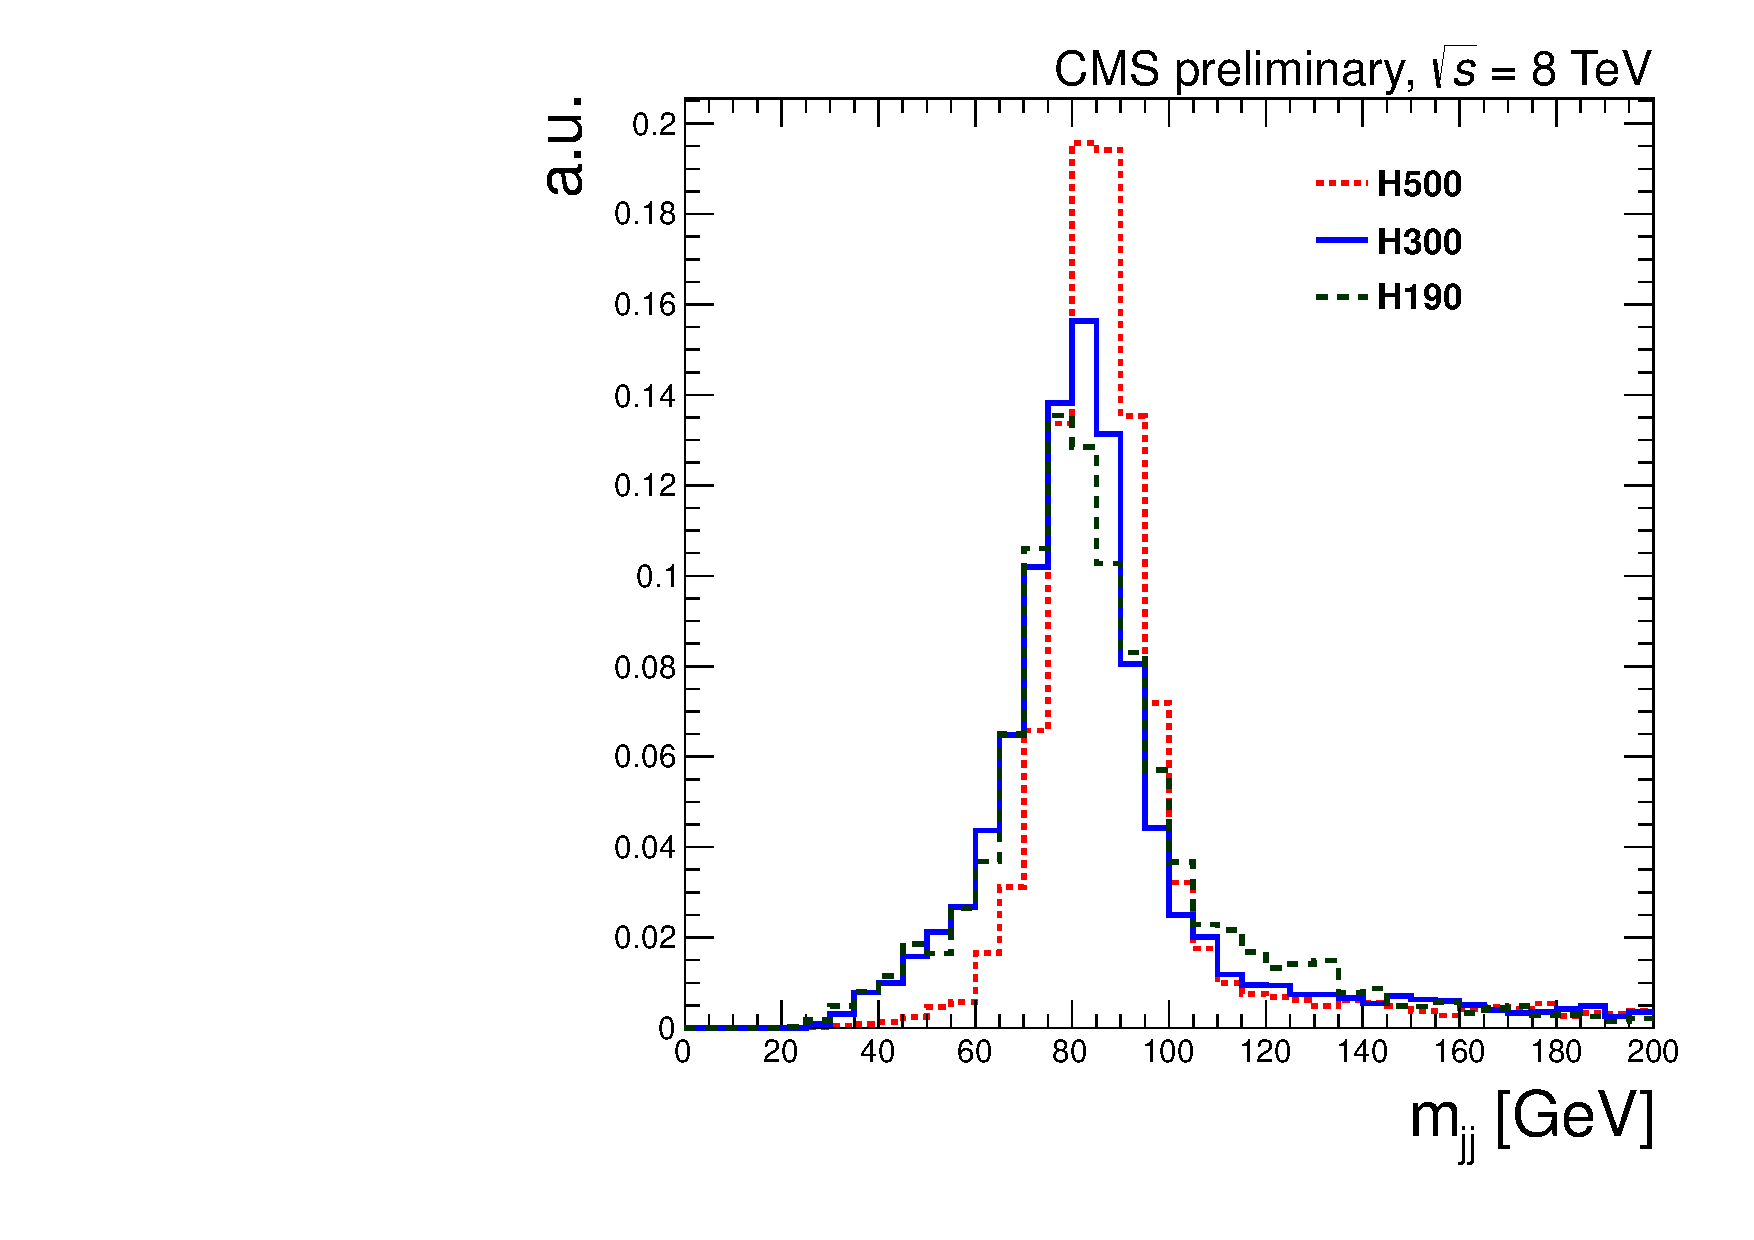
\includegraphics[width=0.6\linewidth]{plots/masses.pdf}
  \caption{The $mjj$ signal shape for an Higgs mass of 200, 400 and 600~\GeV, muon plus 2-jets category.
  All the distributions are normalized to unity. }
  \label{fig:mjj_signals}
  \end{center}
\end{figure}

% ---- ---- ---- ---- ---- ---- ---- ---- ---- ---- ---- ---- ---- ---- ---- ---- ---- ---- ---- ---- ---- ----

\section{The four-body mass shapes}%%% for the likelihood analysis}
\label{sec:4bodymass}
For the limit extraction, the contribution of each background in the signal region
($65\GeVnn < m_{jj} < 95\GeVnn$) is described by the expected shape and normalization.

The four-body mass shape of the W+jets contribution is extracted from data as a mixture of the
shape measured in two signal-free regions, namely an upper sideband (SBH,
$95\GeVnn <m_{jj} < 115\GeVnn$ ) and a lower sideband (SBL, $55\GeVnn <m_{jj} < 65\GeVnn$):

\begin{equation}
m_{\textnormal{WW}_i}^{j} = (1-\alpha^j) \cdot m_{\textnormal{SBH}_i}^j + \alpha^j \cdot  m_{\textnormal{SBL}_i}^j~,
\label{EqnAlpha}
\end{equation}

where the index $j$ refers to each of the 48 mass spectra and 
$i$ to the bins in the four-body mass. 
The $\alpha$ factor is chosen for each Higgs mass hypotheses on 
the simulation by minimizing the $\chi^2$ between the extrapolated 
shape in the signal region and the expected one. 
The distributions of the extrapolated W+jets background in the signal 
region are shown in
Figure~\ref{fig:Wjets_dd_example} (muon channel) with selections  
optimized for Higgs mass hypotheses of 190\GeVnn, 300\GeVnn, and 500\GeVnn. 
Because of the low statistics, the shapes are regularized by
means of an exponential fit (solid curve). 
Uncertainties in the $\alpha$ factor and in the decay constant 
of the exponential are utilized to derive the systematic band.

\begin{figure}[!t]
  \centering
  \subfigure[]{
  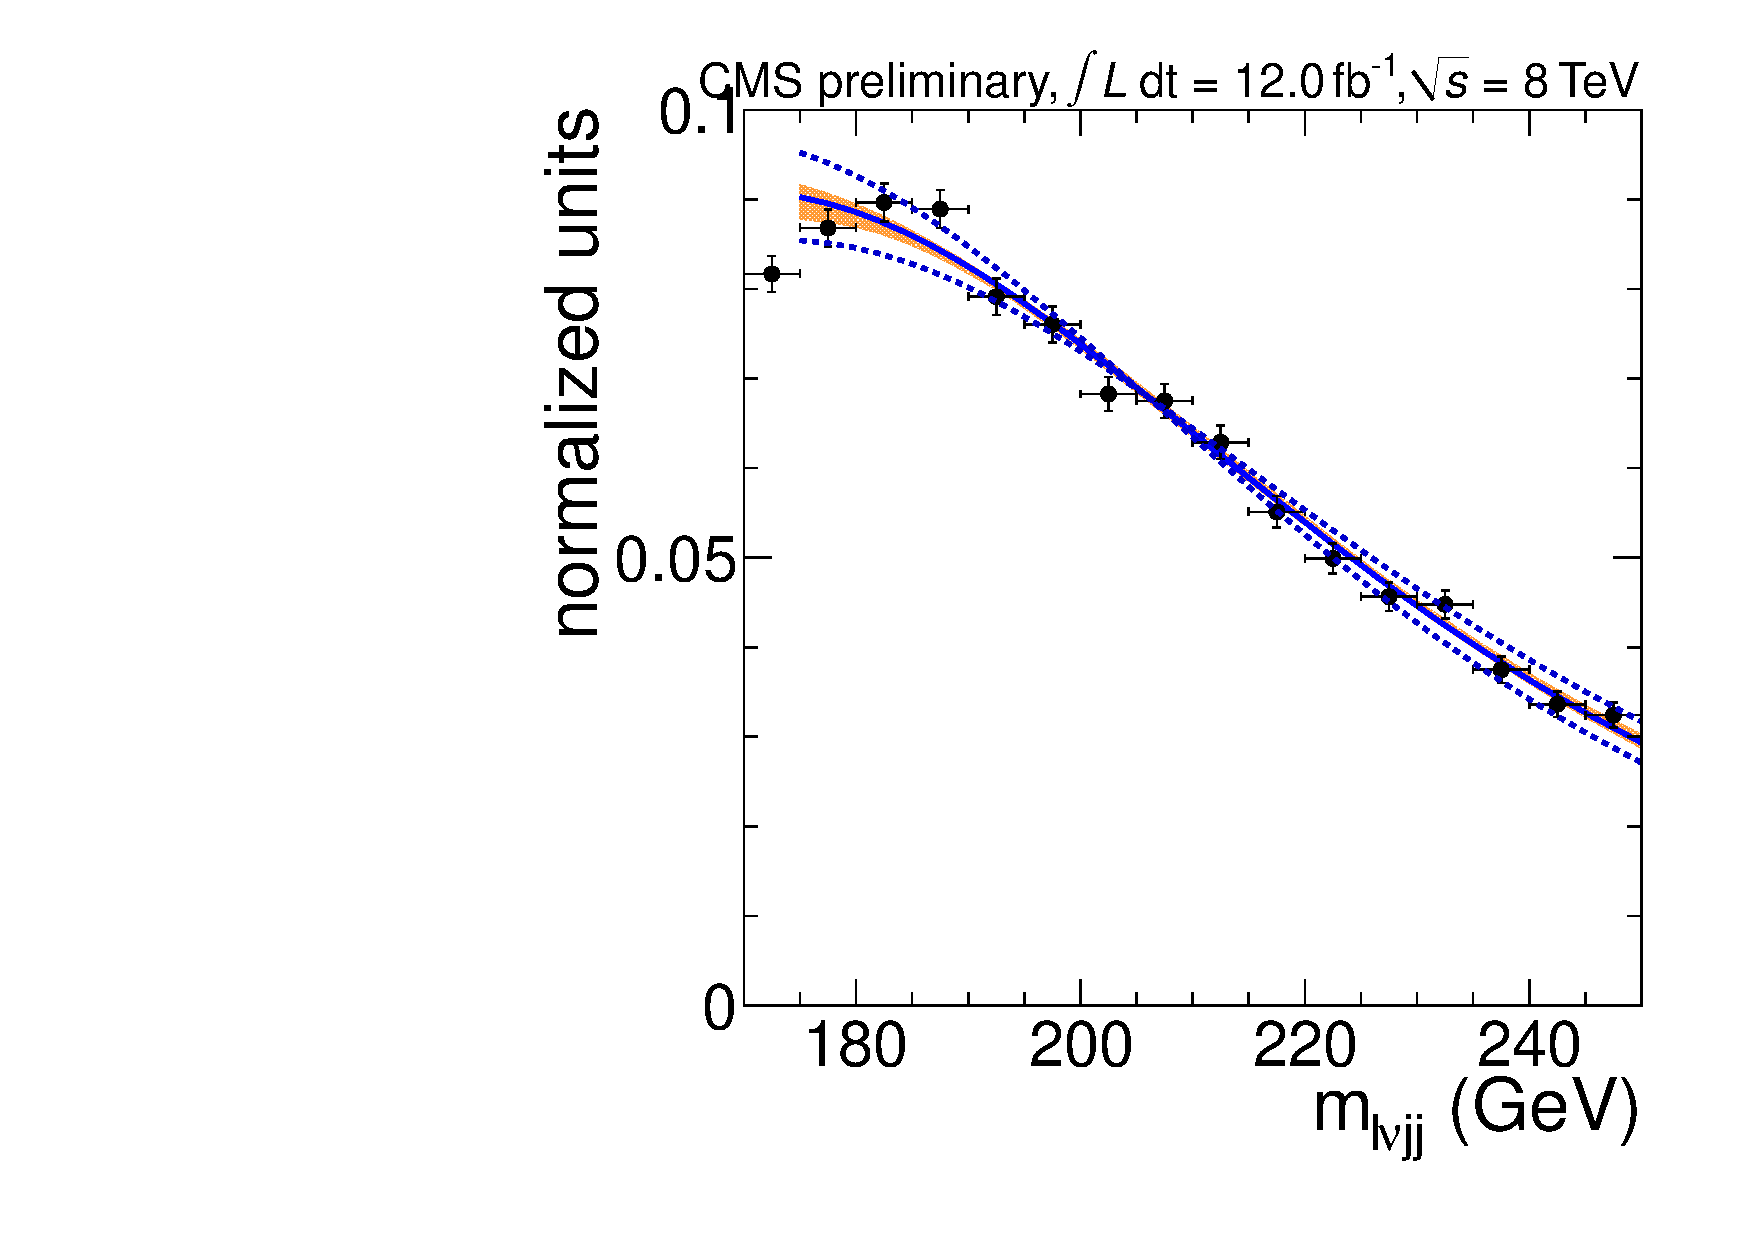
\includegraphics[width=0.32\textwidth]{plots/H190_Mlvjj_Muon_2jets_WpJShape.pdf}
  }  
  \subfigure[]{ 
  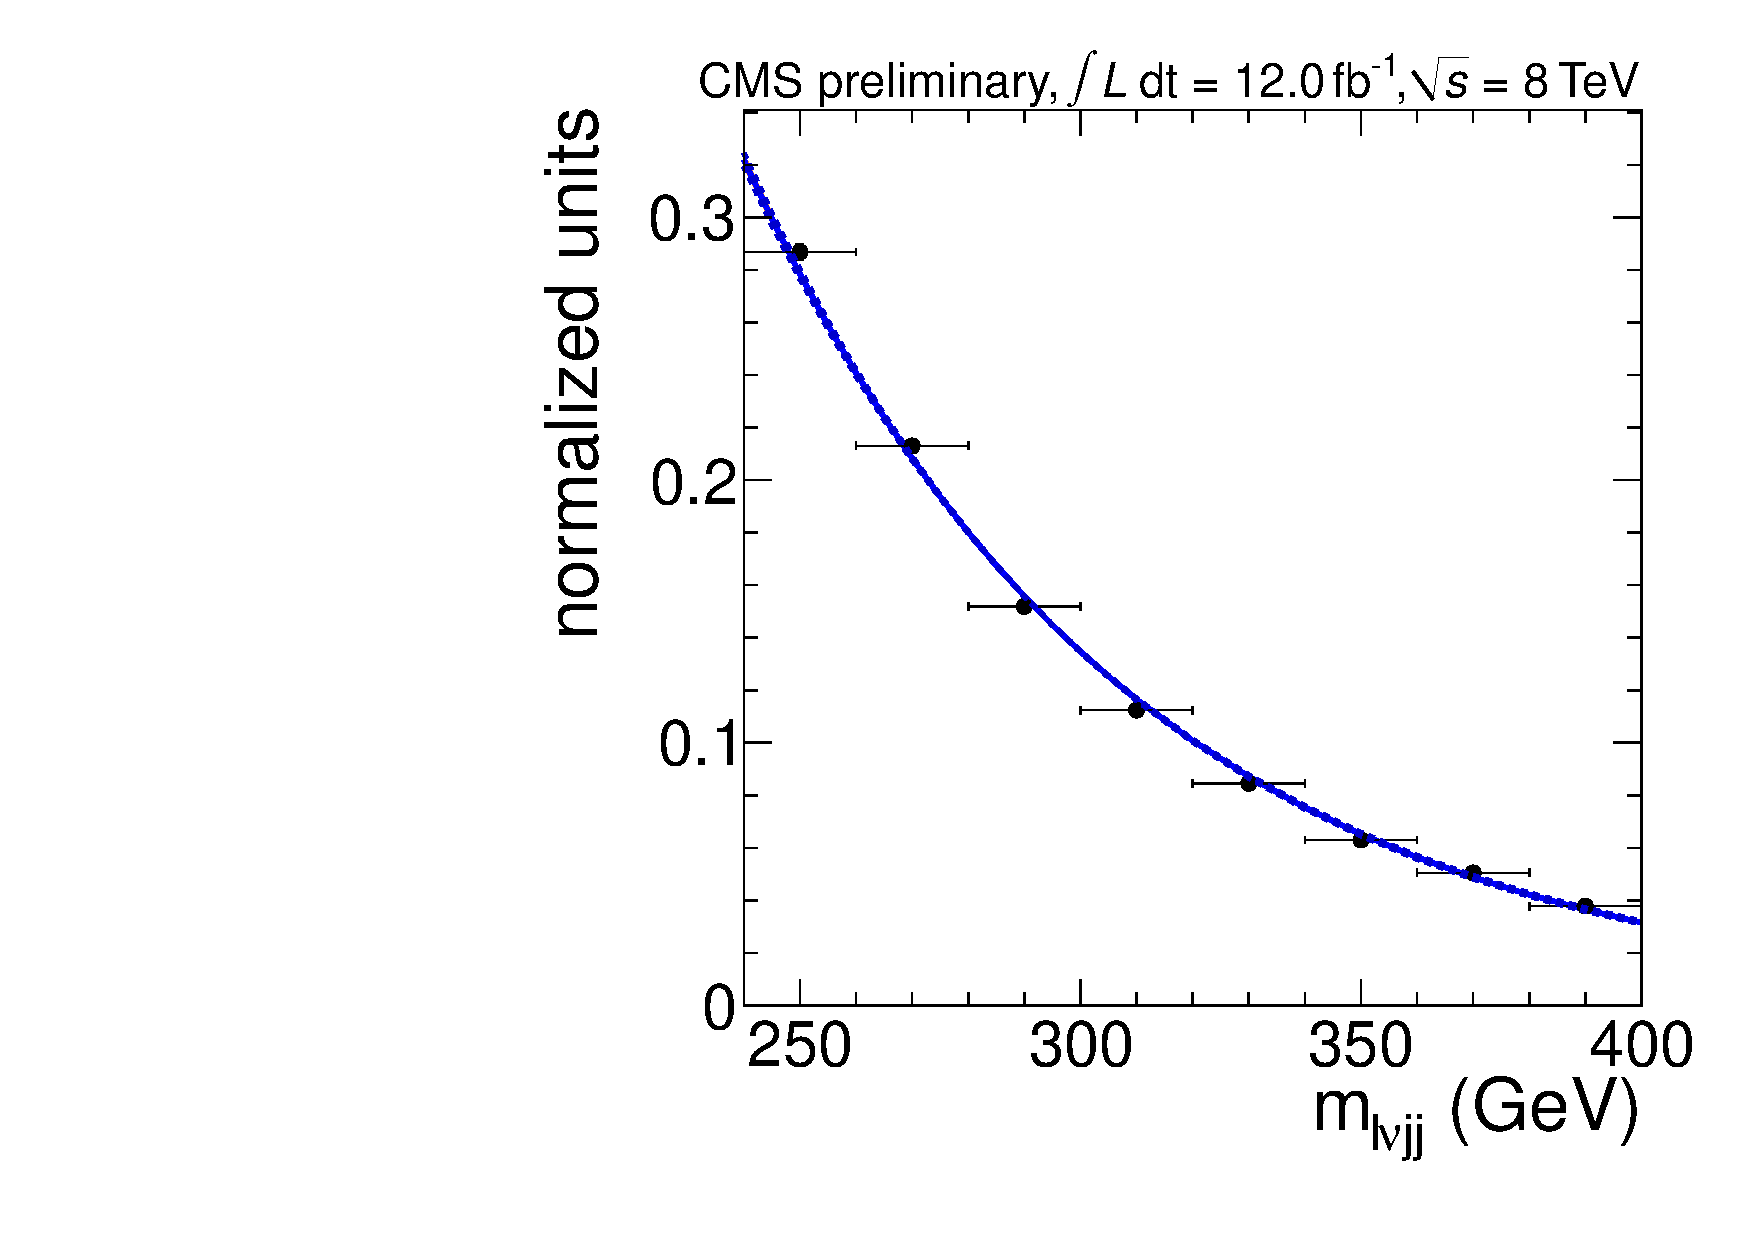
\includegraphics[width=0.32\textwidth]{plots/H300_Mlvjj_Muon_2jets_WpJShape.pdf}
  }  
   \subfigure[]{ 
  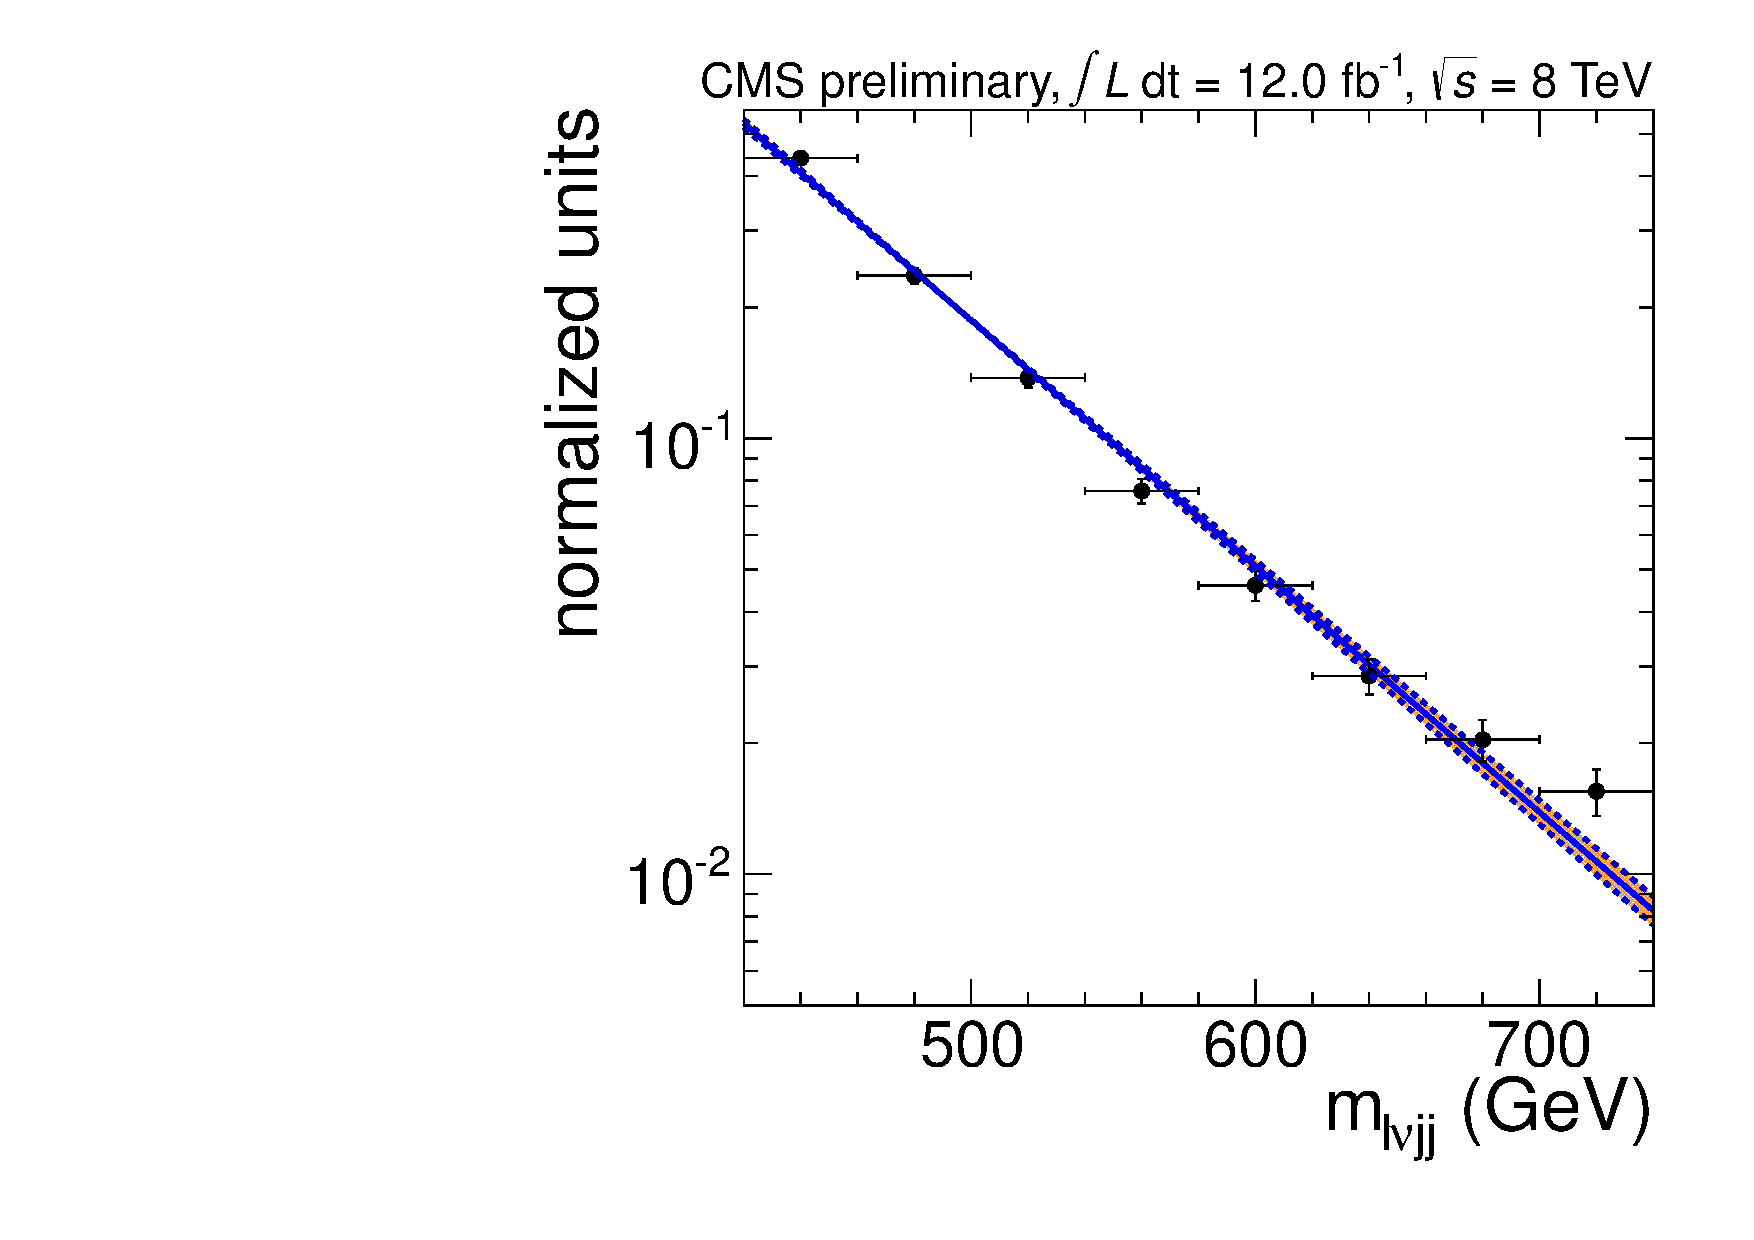
\includegraphics[width=0.32\textwidth]{plots/H500_Mlvjj_Muon_2jets_WpJShape_log.pdf}
  }   
  \caption{\label{fig:Wjets_dd_example}The distribution of the 
  extrapolated background shape in the
  signal region for the Higgs mass hypothesis of 190\GeVnn (a), 
  300\GeVnn (b), and 500\GeVnn (c),
  for the muon plus 2-jets category. The 500\GeVnn plot is given in logarithmic scale. 
  The black markers represent the extrapolated points, while the blue curve
  is the smooth parametrization using an exponential function. 
  The dashed bands show the envelope of
  the systematic uncertainty in the shape extrapolation.} 
\end{figure}

The four-body mass shape for multijet background events is obtained 
from data as well, by selecting a control sample of non-isolated 
leptons and relaxing the $\MET$ threshold and identification requirements. 
The fraction of multijet events in data
is computed from a fit to W transverse mass. 
For muons, the multijet fraction is negligible, while for 
electrons it is several percent depending on the jet multiplicity 
in the event. 
All other background categories use the $m_{\ell\nu{}jj}$
shape predicted by their respective Monte Carlo samples. The
$m_{\ell\nu{}jj}$ invariant mass distribution in the signal region is
shown in Figure~\ref{fig:mlvjj_mH350} for the muon plus 2-jet channel, with
selections optimized for Higgs mass hypotheses 190\GeVnn, 300\GeVnn,
and 500\GeVnn.

\begin{figure}[!t]
  \centering
  \subfigure[]{
  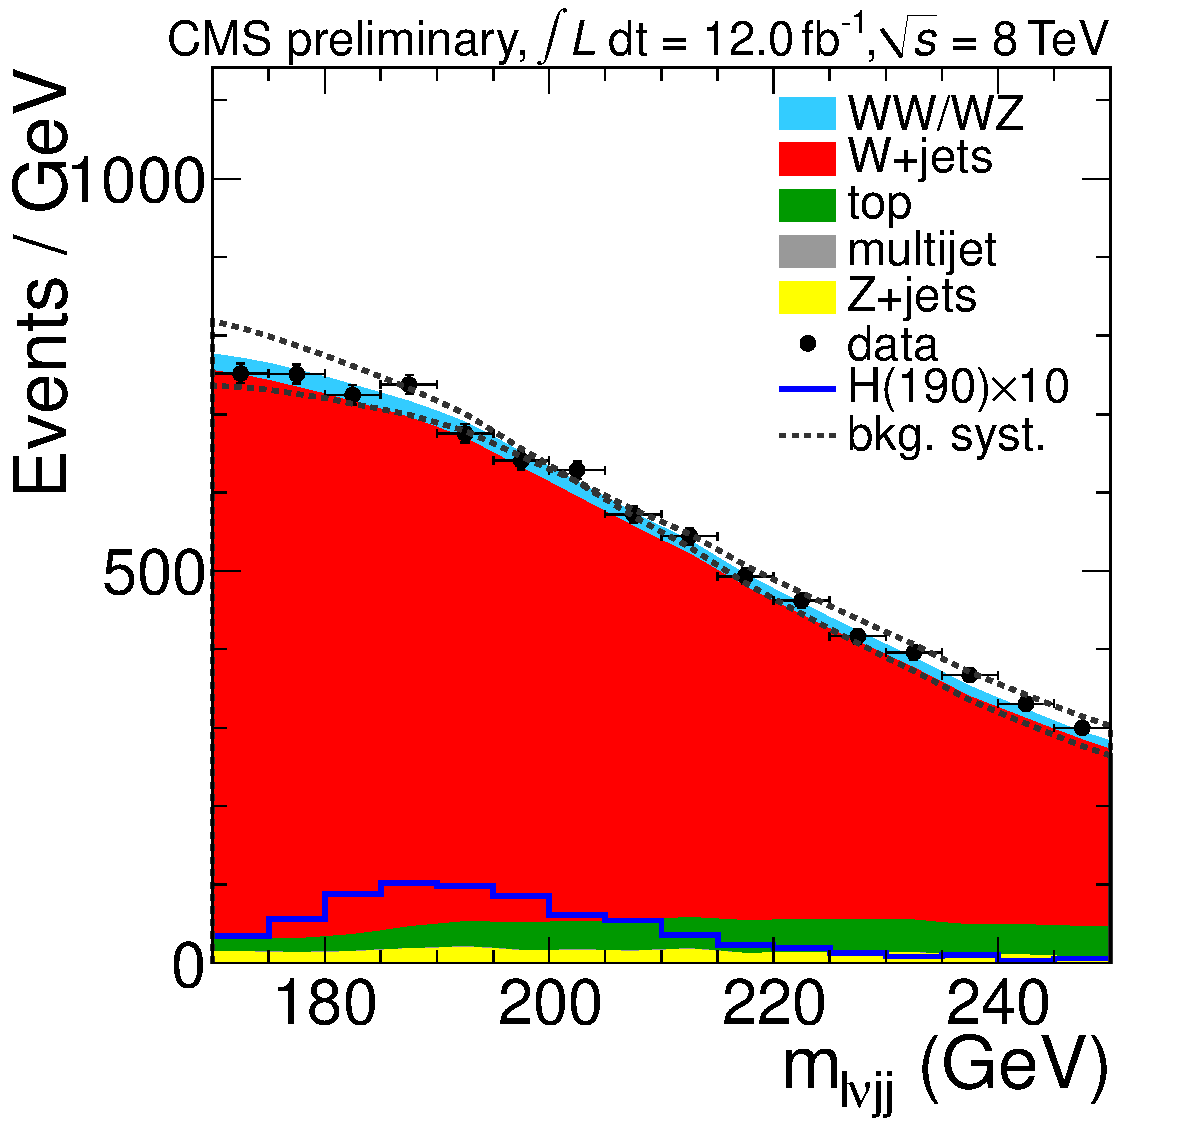
\includegraphics[width=0.32\textwidth]{plots/H190_Mlvjj_Muon_2jets_Stacked.pdf}
  }  
  \subfigure[]{ 
  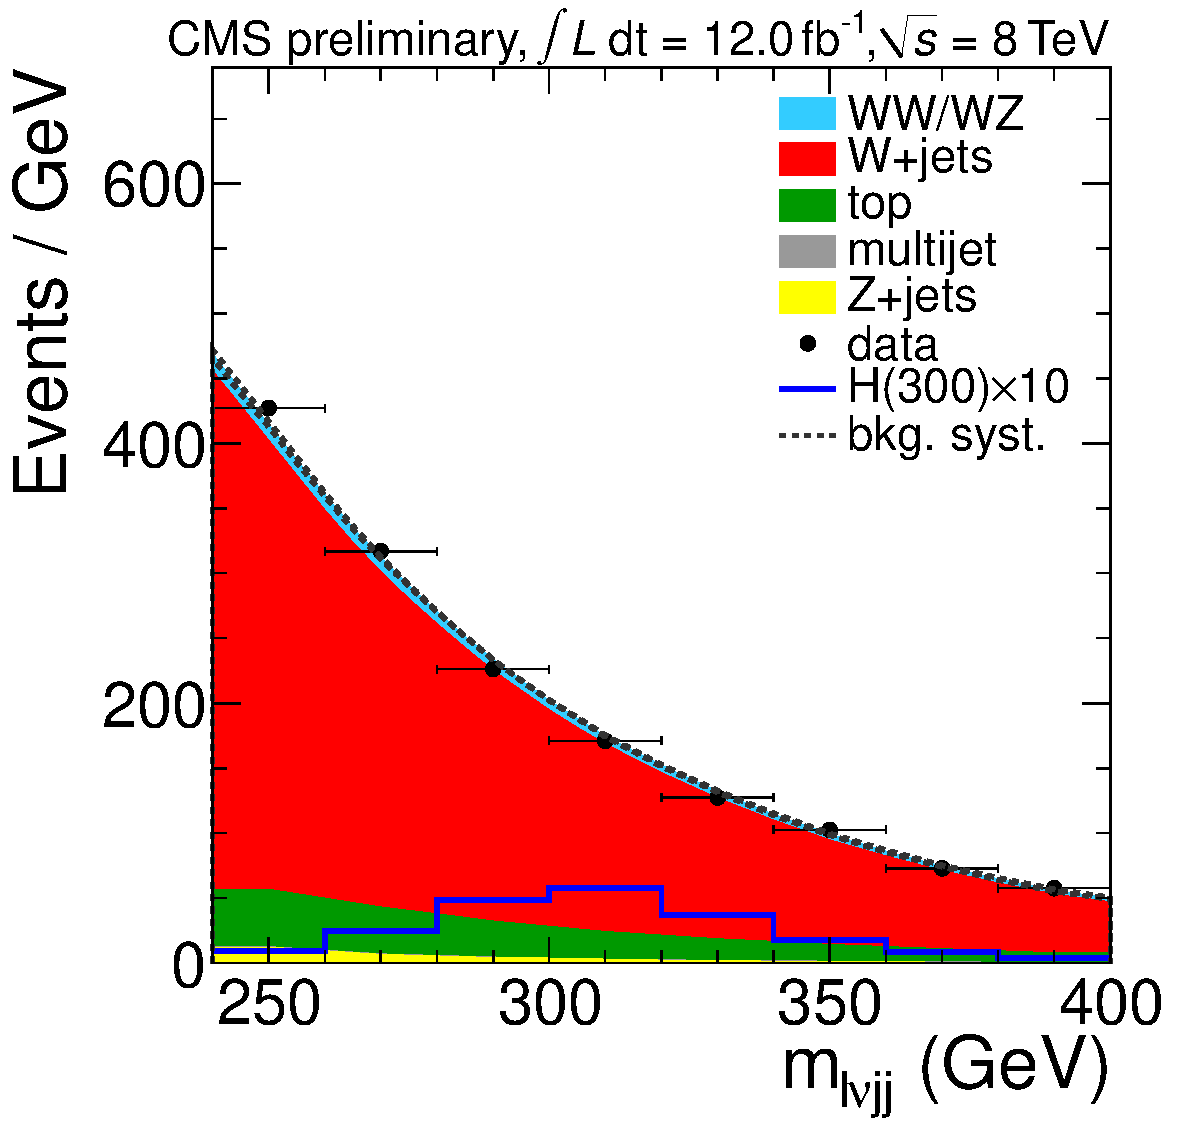
\includegraphics[width=0.32\textwidth]{plots/H300_Mlvjj_Muon_2jets_Stacked.pdf}
  }  
  \subfigure[]{ 
  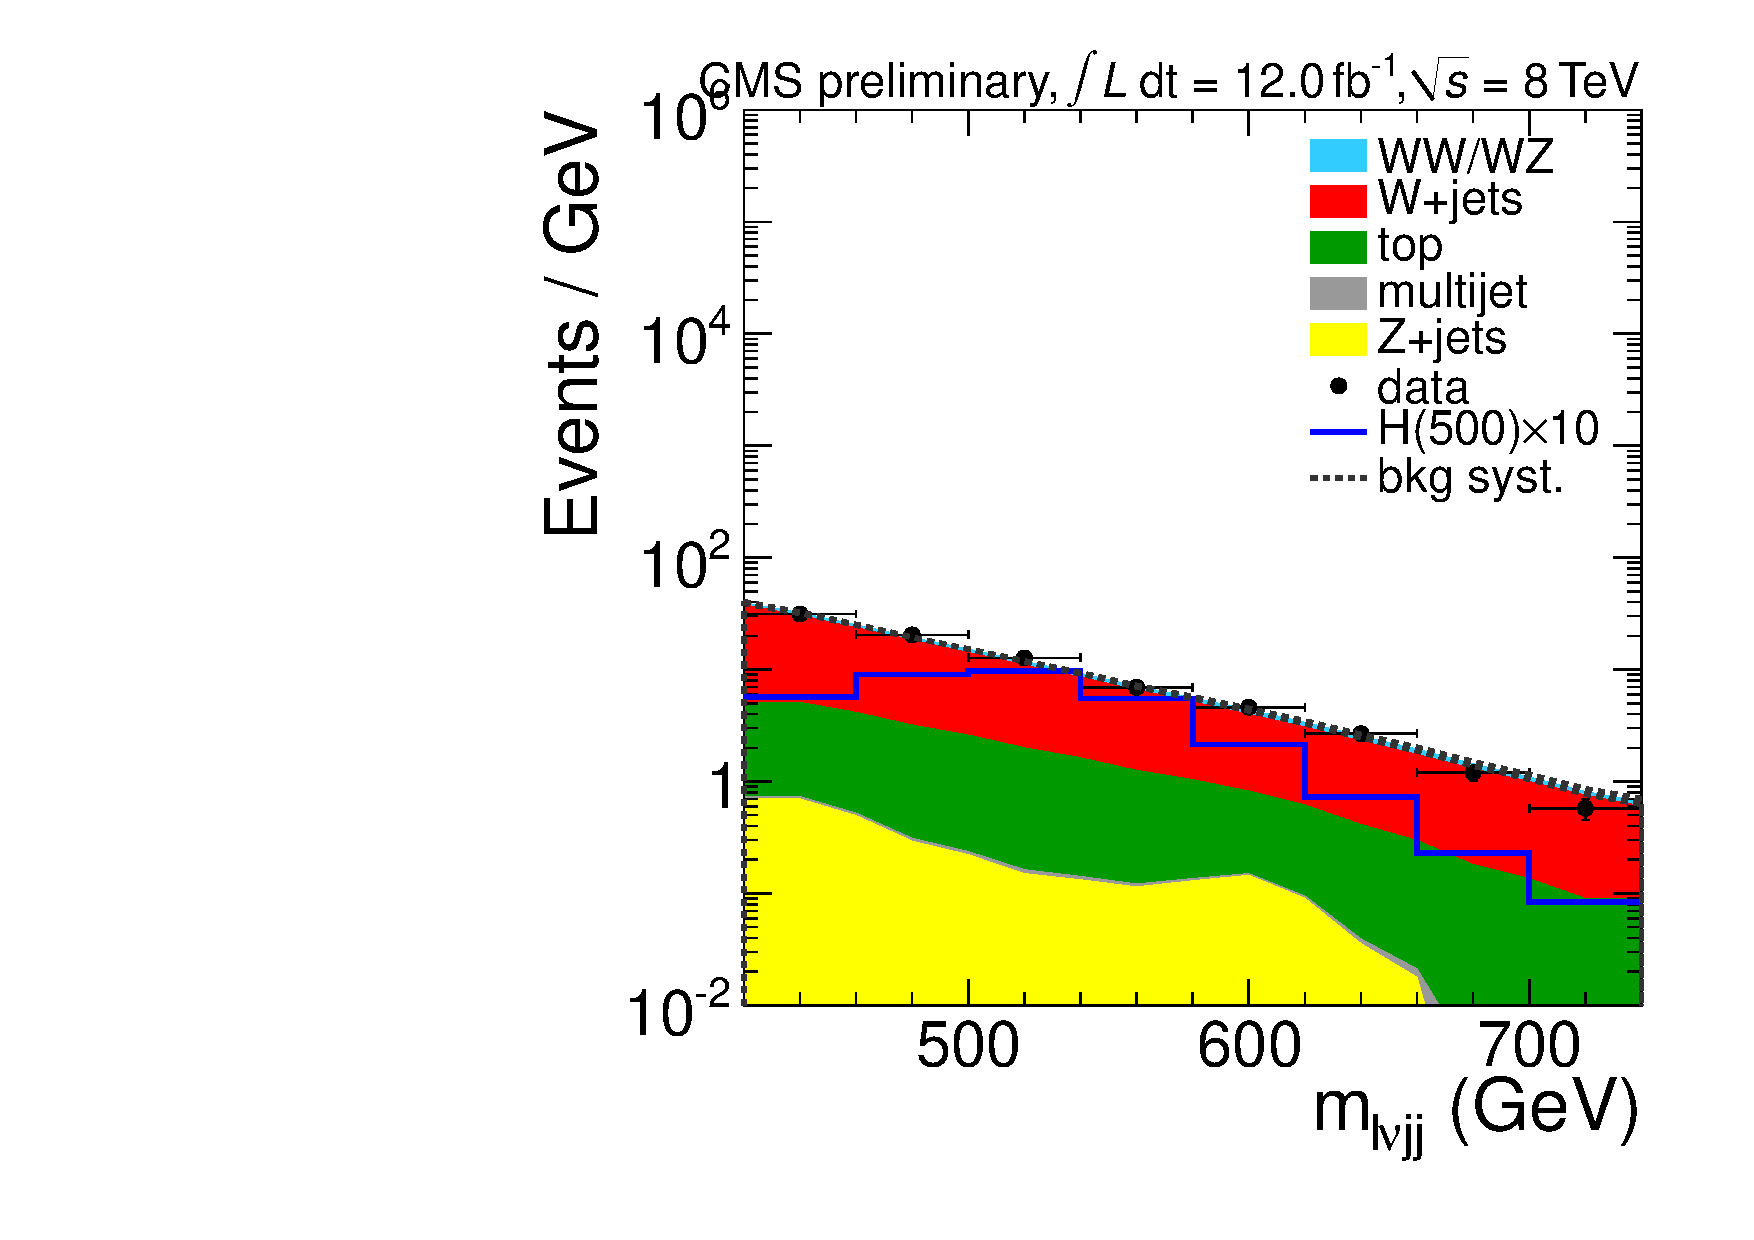
\includegraphics[width=0.32\textwidth]{plots/H500_Mlvjj_Muon_2jets_Stacked_log.pdf}
  }   
%%\vspace*{1mm} \\
%%  \subfigure[]{
%%  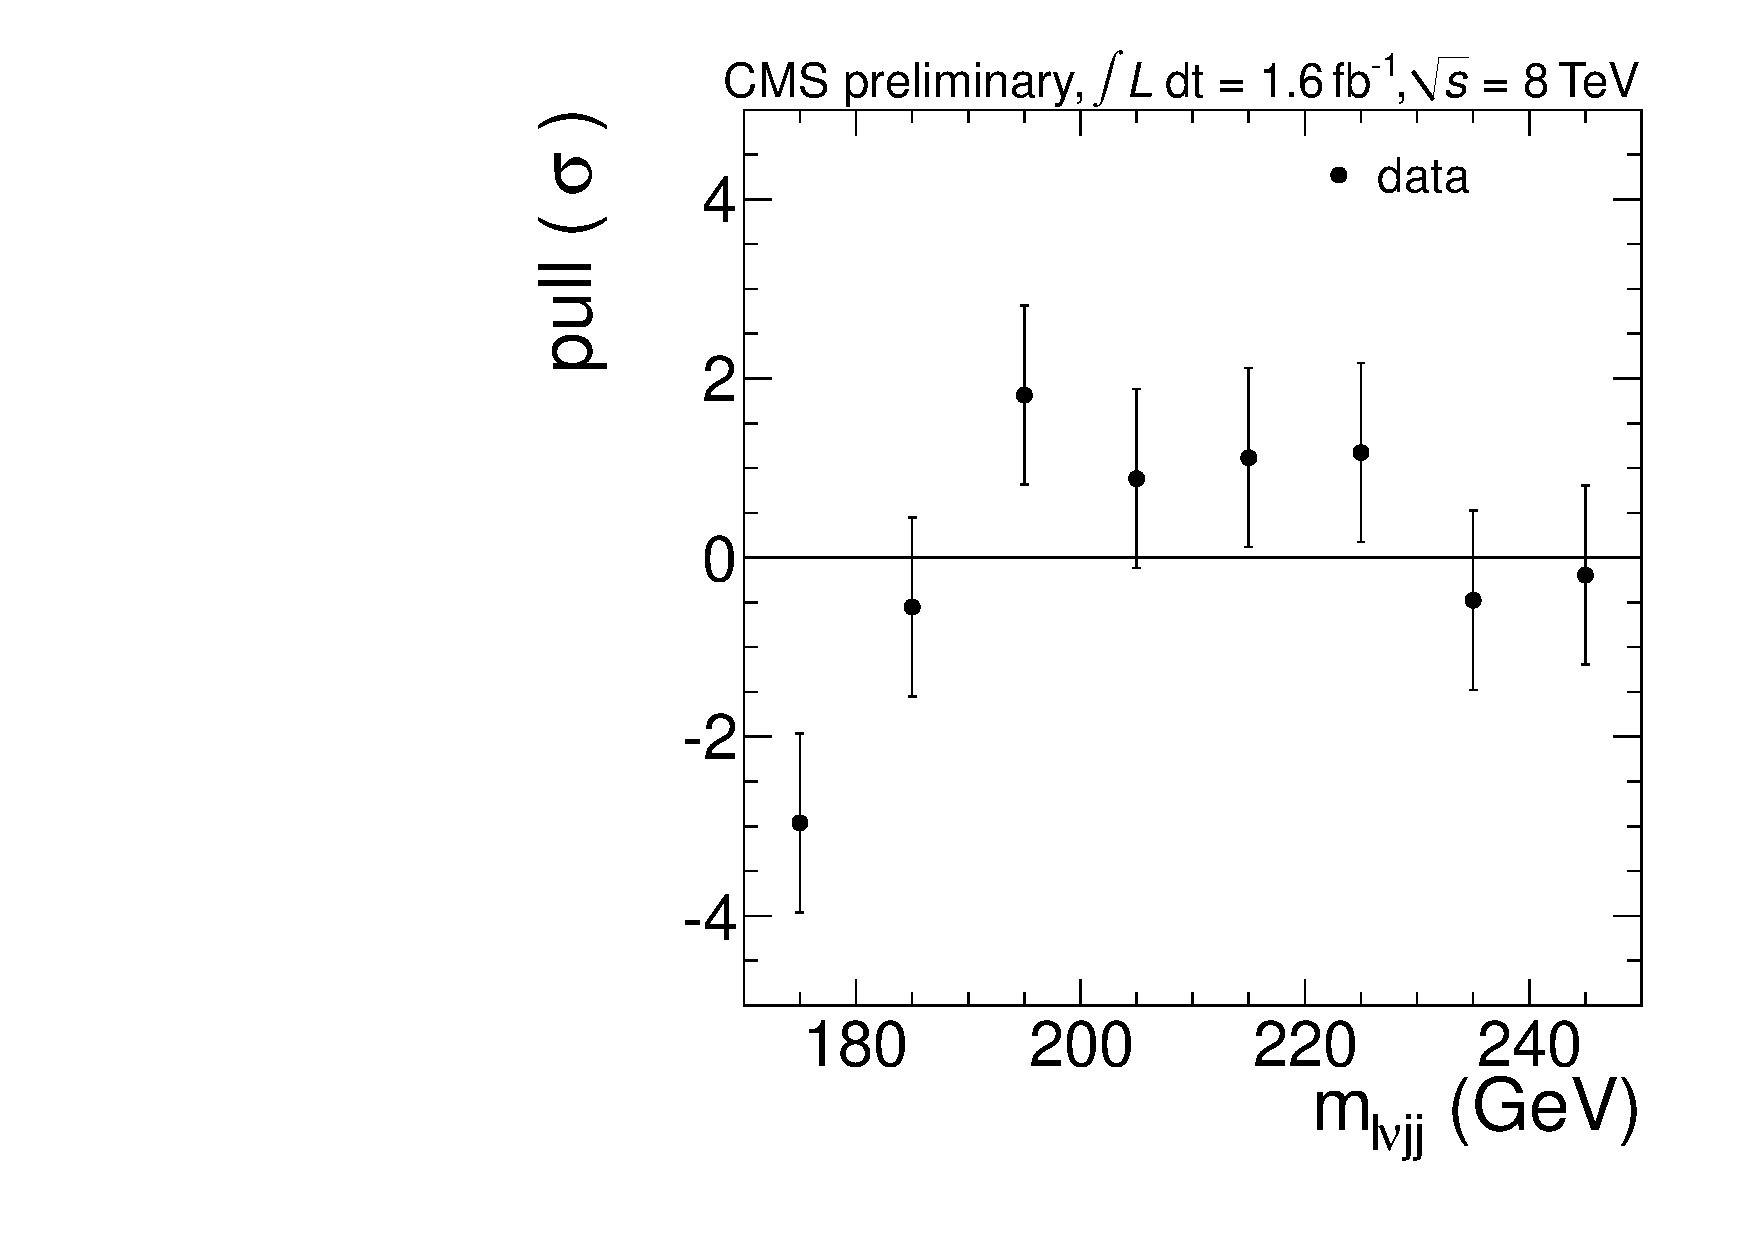
\includegraphics[width=0.32\textwidth]{plots/H190_Mlvjj_Muon_2jets_Pull.pdf}
%%  }  
%%   \subfigure[]{ 
%%  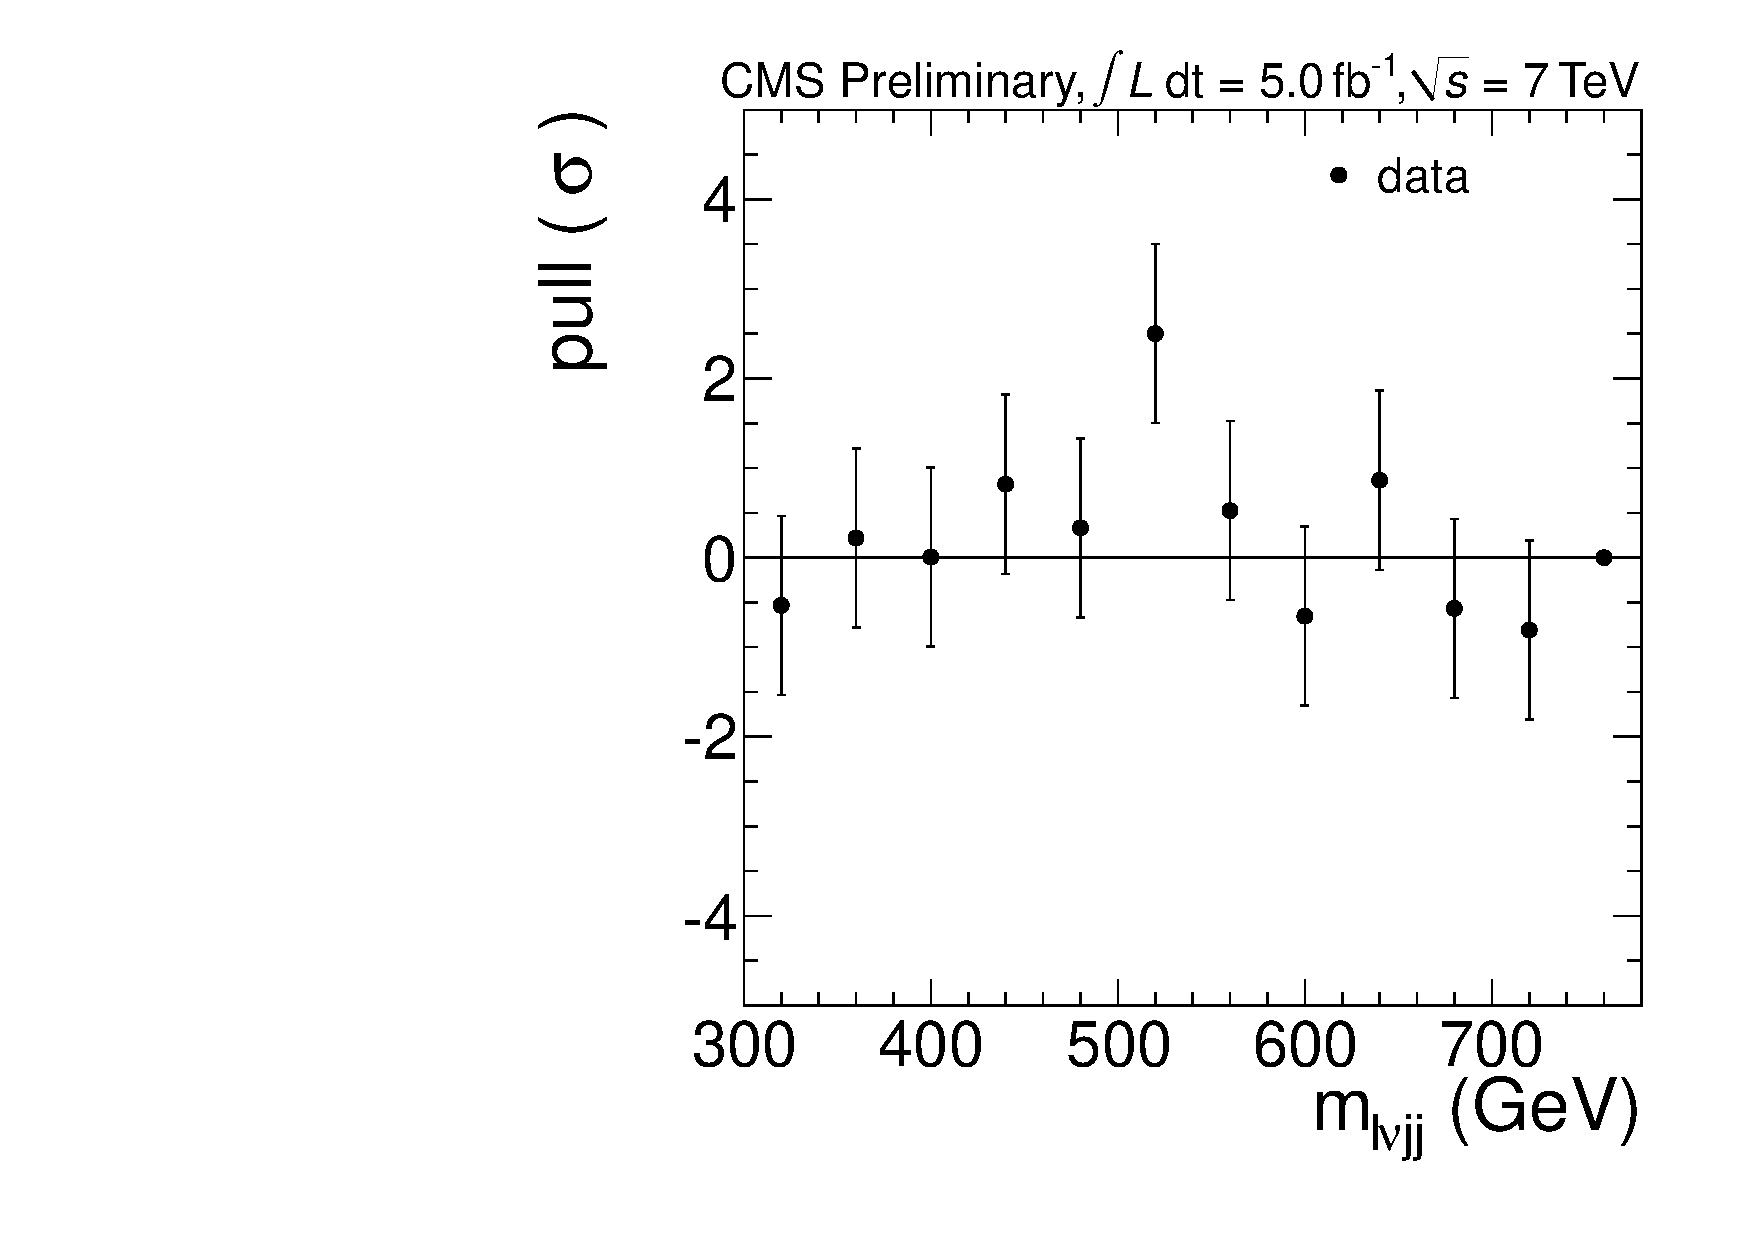
\includegraphics[width=0.32\textwidth]{plots/H350_Mlvjj_Muon_2jets_Pull.pdf}
%%  }   
%%  \subfigure[]{ 
%%  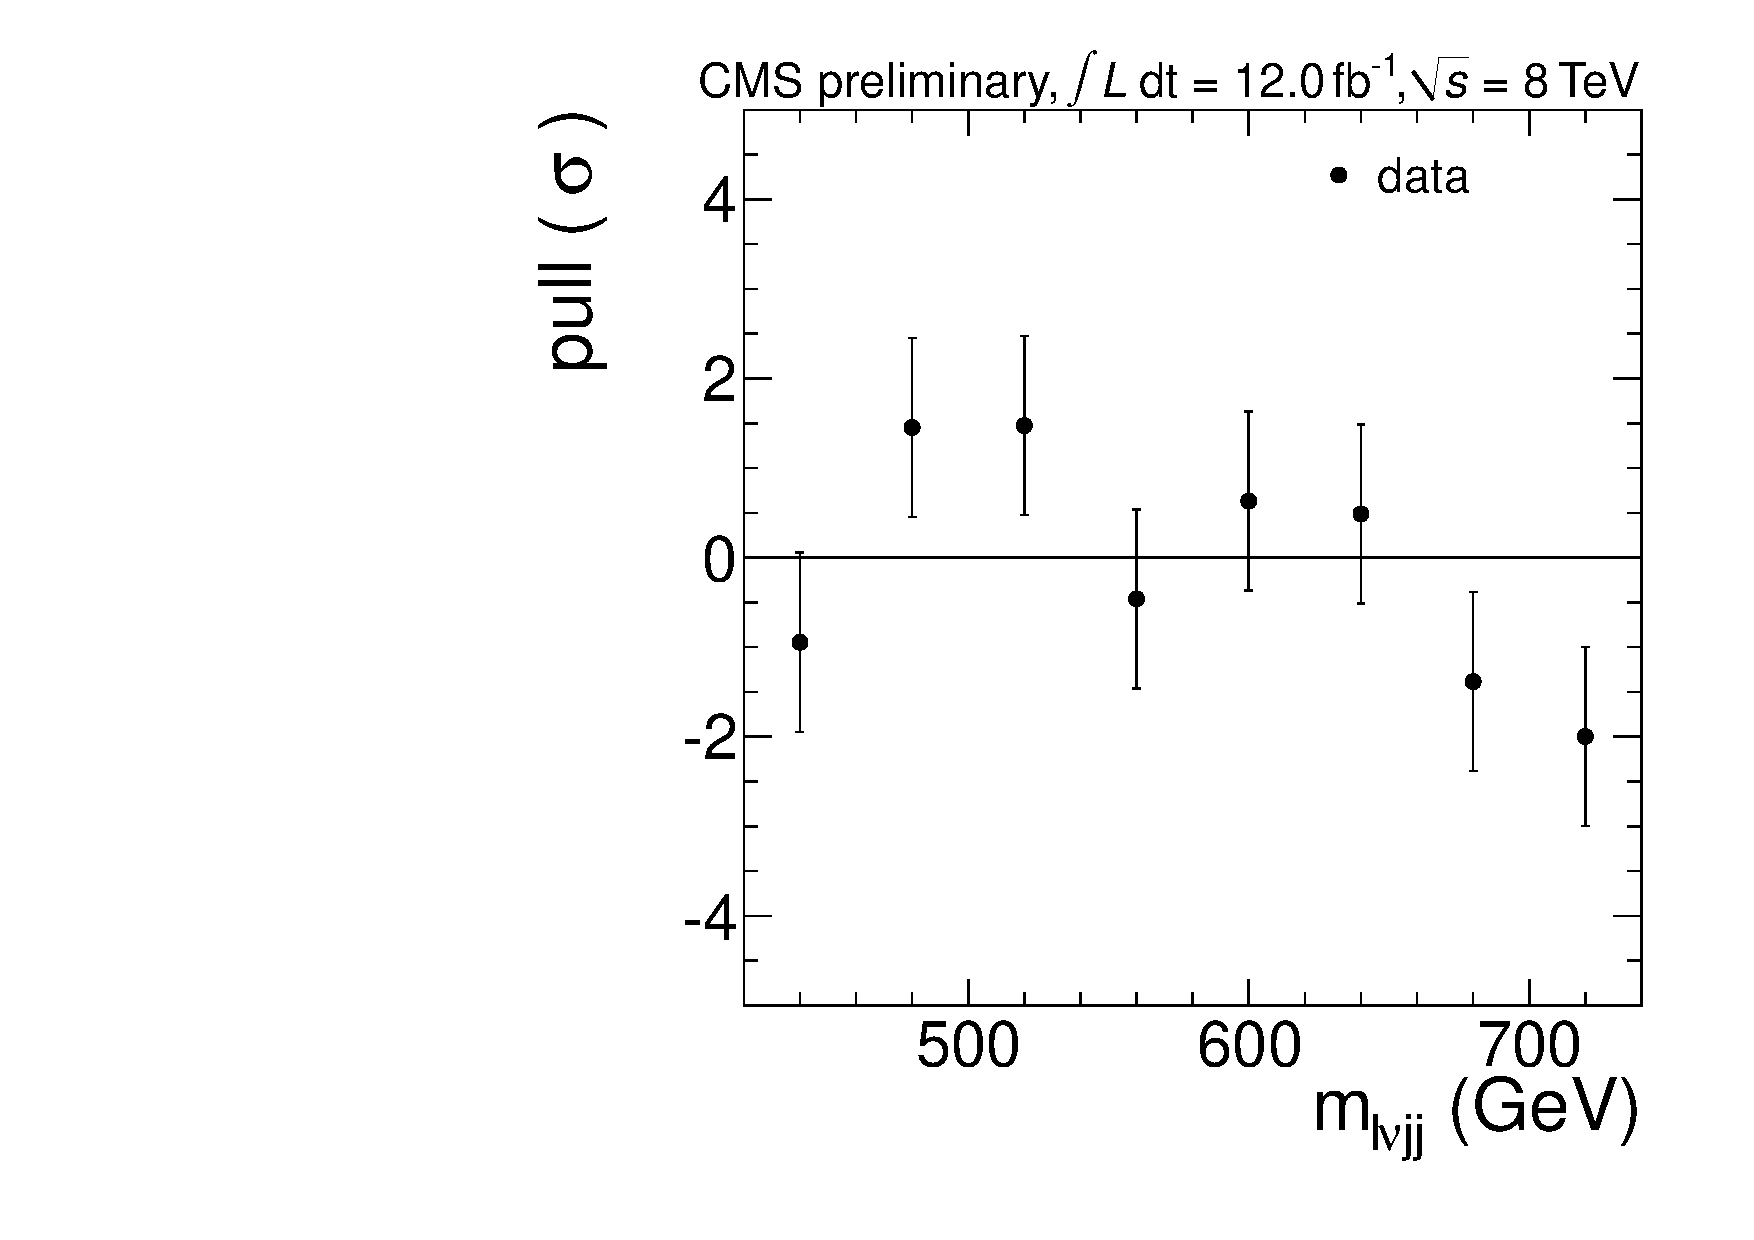
\includegraphics[width=0.32\textwidth]{plots/H500_Mlvjj_Muon_2jets_Pull.pdf}
%%  }   
%%  \caption{\label{fig:mlvjj_mH350}
%%  The WW invariant mass distribution with the fit projections, for the 
%%  muon 2-jet category, after selections optimized for the Higgs mass hypotheses of 
%%  190\GeVnn (a, d), 350\GeVnn (b, e), and 500\GeVnn (c, f). 
%%  The top row shows the distribution of the
%%  $m_{\ell\nu{}jj}$ invariant mass distribution in the signal region $65\GeVnn < m_{jj} < 95\GeVnn$.
%%  With the kinematic selection used, we expect about 55, 79, and 27 Higgs signal events 
%%  in the three distributions, respectively.
%%  The bottom row shows pull distribution computed as [(Data - Background)/ Background uncertainty].}
  \caption{\label{fig:mlvjj_mH350}
  The WW invariant mass distribution with the fit projections in the signal region $65\GeVnn < m_{jj} < 95\GeVnn$, for the 
  muon plus 2-jets category, after selections optimized for the Higgs mass hypotheses of 
  190\GeVnn (a), 300\GeVnn (b), and 500\GeVnn (c).
  The error bars correspond to the statistical uncertainties. 
  Systematic uncertainties are not shown here. 
  The main systematic uncertainty comes from W+jets shape extraction, 
  and is shown in Fig.~\ref{fig:Wjets_dd_example}. 
  Uncertainties in the signal strength and lineshape are listed in 
  Table~\ref{tab:signalSyst}. 
}
\end{figure}

% ---- ---- ---- ---- ---- ---- ---- ---- ---- ---- ---- ---- ---- ---- 

\section{Systematic uncertainties}
\label{sec:systematics}
Systematic uncertainties considered in this analysis are listed in 
Table~\ref{tab:signalSyst}.
Because of the background dominance,  
the largest source of systematic uncertainty is the shape 
uncertainty of the W+jets $m_{\ell\nu jj}$ distribution 
described in the previous section. 
The only other uncertainty assigned to background 
is the normalization uncertainty that 
comes from the $m_{jj}$ fit described in Section~\ref{sec:mjjfit}.


% SIGNAL SYSTEMATICS
%%% After rescaling the transverse momentum distribution 
%%% of the Higgs boson to the HQT prediction~\cite{Bozzi:2005wk}, 
We follow the LHC Higgs 
Cross Section Working Group~\cite{LHCXSWG}
%%PDF4LHC~\cite{Botje:2011sn,Alekhin:2011sk,Lai:2010vv,Martin:2009iq,Ball:2011mu} 
recommendations for the uncertainties on the production cross-section
of the Higgs boson, and for PDF uncertainties propagated to the signal
acceptance within our selections.  The uncertainty in scale caused by
exclusive binning in the 2-jet and 3-jet categories~(\cite{CLS2},
Appendix C) is accounted for. The uncertainty in the interference
reweighting procedure described above is implemented as a shape
variation on the signal $m_{\ell\nu jj}$ distribution.
Figure~\ref{fig:sigshapeintfunc} shows an example of this variation
for a Higgs mass of 600~\GeV, for which, of all the mass hypotheses
considered, the effect is largest.

\begin{figure}[t!]
  \begin{center}
    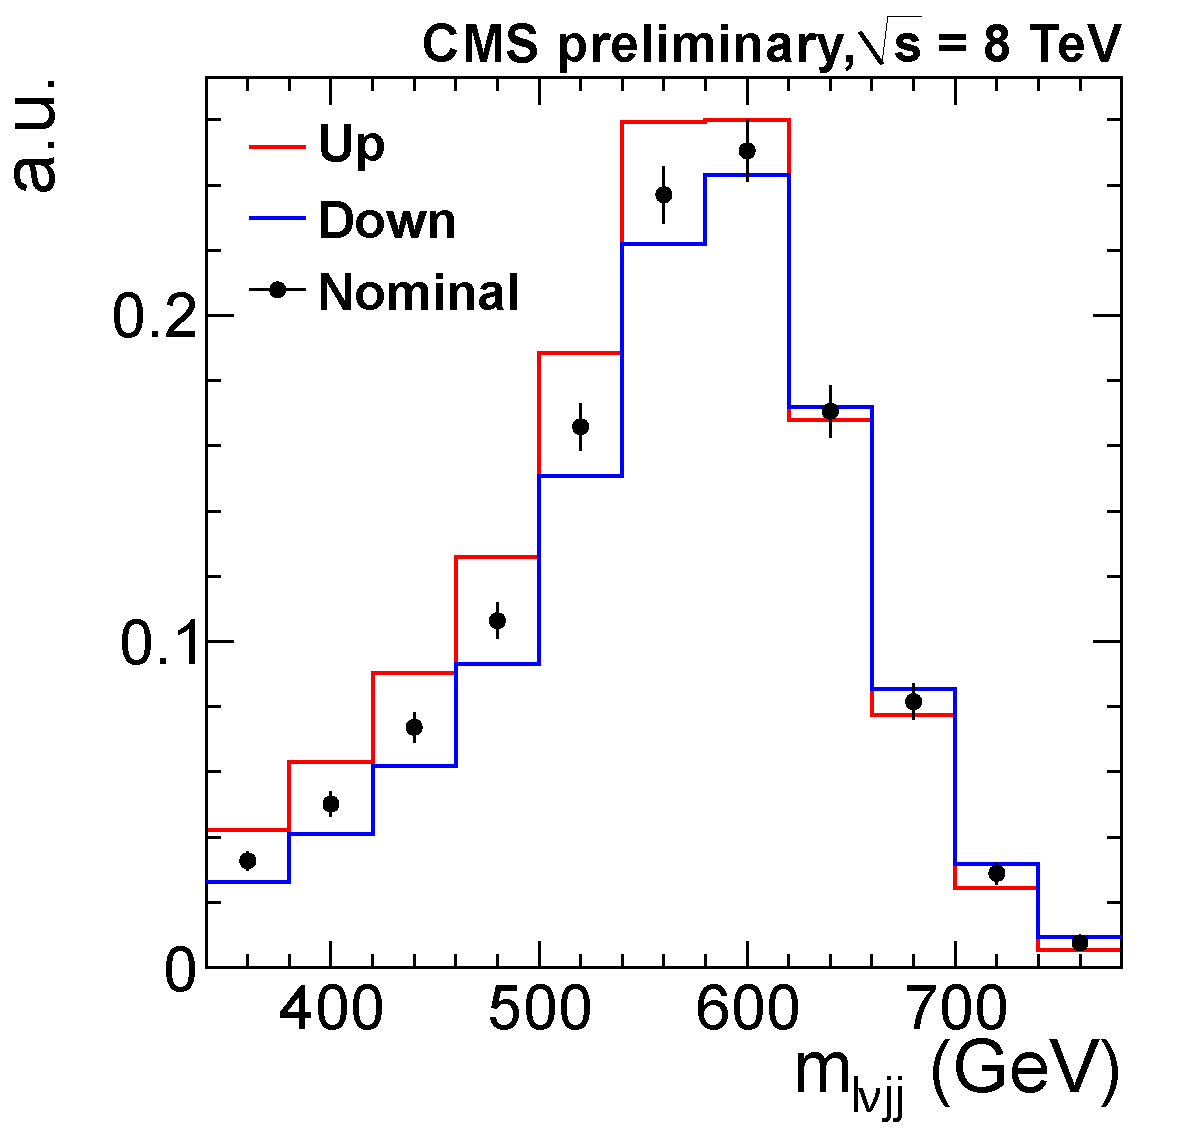
\includegraphics[width=0.5\linewidth]{plots/H600_Muon_2jets_Signal_Shape.pdf}
  \caption{The shape variation for the signal $m_{\ell\nu jj}$ distribution,
  for a Higgs mass of 600~\GeV, muon plus 2-jets category. }
  \label{fig:sigshapeintfunc}
  \end{center}
\end{figure}

The uncertainty due to luminosity is considered~\cite{lumiPAS}.
%%% as well as the one due to the measurement of the number of pile-up
%%% events in data. 
The uncertainties on the reconstruction, identification
and trigger efficiencies are extracted from the corresponding
measurements, performed with a tag-and-probe~\cite{VBTF} approach.  
The uncertainty on the jet energy measurements is accounted for by 
using hadronically decaying W boson in highly pure \ttbar semi-leptonic 
events~\cite{TOP-11-015}.
The uncertainty is calculated by comparing the reconstructed hadronic
W mass in a \ttbar enriched sample between data and Monte Carlo.
We compute the systematic uncertainty in the 
Higgs signal efficiency associated with the likelihood selection 
on the simulation sample by using a control sample in data. 
A highly pure sample of top pair events is obtained by requiring 
the presence of two extra b-tagged jets.  
These events are good proxies for 
our signal because in both cases the primary production mechanism 
is gluon-gluon 
fusion and the semi-leptonic final state contains decays of two W bosons. 
We take the relative difference in efficiency between data and simulation 
for top pair events after all the selections as an estimation of systematic 
uncertainty in signal efficiency. 
This accounts for 10\% uncertainty in signal strength.

%%%%%%%
 \begin{table}[h!]
   \begin{center}
   \begin{tabular}{l|c}
  \hline
  \hline
  Source of uncertainty & Magnitude \\
  \hline   
   Background  $m_{\ell\nu jj}$ shape    & See Fig.~\ref{fig:Wjets_dd_example}\\
   Background  normalization             & 0-2\% \\      
  \hline    
   Higgs boson cross-section             & 13-15\% \\
   Theory acceptances (PDF)              & 1-2\% \\                  
%%   Higgs boson line shape                & 0-30\% \\
   Scale uncertainties from jet binning  & 4-28\% \\
   Luminosity                            & 4.4\% \\
   Lepton selection eff.                 & 1-2\% \\
   Lepton trigger eff.                   & 1\% \\
  %%Pile-up                              & $<$1\% \\
   Jet energy scale, resolution, and \MET & $<$1\% \\
   Likelihood selection                  & 10\% \\
   Signal shape (interference)           & See Fig.~\ref{fig:sigshapeintfunc} \\
  \hline
  \hline
   \end{tabular}
   \end{center}
   \caption{Sources of systematic uncertainties considered in the analysis, 
   with the corresponding magnitude, for the limit extraction.} 
   \label{tab:signalSyst}
 \end{table}
%%%%%%%
% ---- ---- ---- ---- ---- ---- ---- ---- ---- ---- ---- ---- ---- 

\section{Results}
\label{sec:results}
Upper limits on the SM Higgs boson production cross section have 
been calculated. 
We use the modified frequentist construction
CL${}_{\textrm{S}}$~\cite{CLS2, CLS} with profile likelihood as the 
test statistic. 
Based on the expected normalization and shape of the $m_{\ell\nu{}jj}$ 
distribution, for signal and background, and the 
corresponding systematic uncertainties, we generate a large 
number of random pseudo-experiments. 
For each of them, the expected background distribution is generated 
and a likelihood ratio for signal
plus background is calculated. We present 95\% exclusion 
limits on the ratio of the production cross section for the 
Higgs boson compared to the SM expectation in Figure~\ref{fig:exclusion}. 
We exclude at 95\% confidence level the SM Higgs boson in the mass ranges
225--485\GeVnn and 550--600\GeVnn from analyzing 8 TeV data,
while the median expected exclusion range is 220--560\GeVnn.
Combining with 7 TeV results~\cite{HIG-12-003}, we exclude the SM Higgs boson in
the mass ranges
215--490\GeVnn and 525--600\GeVnn
at 95\% confidence level, while the median expected one becomes
170--585\GeVnn.

%%%
\begin{figure}[tbh]
  \begin{center}
    \centerline{
    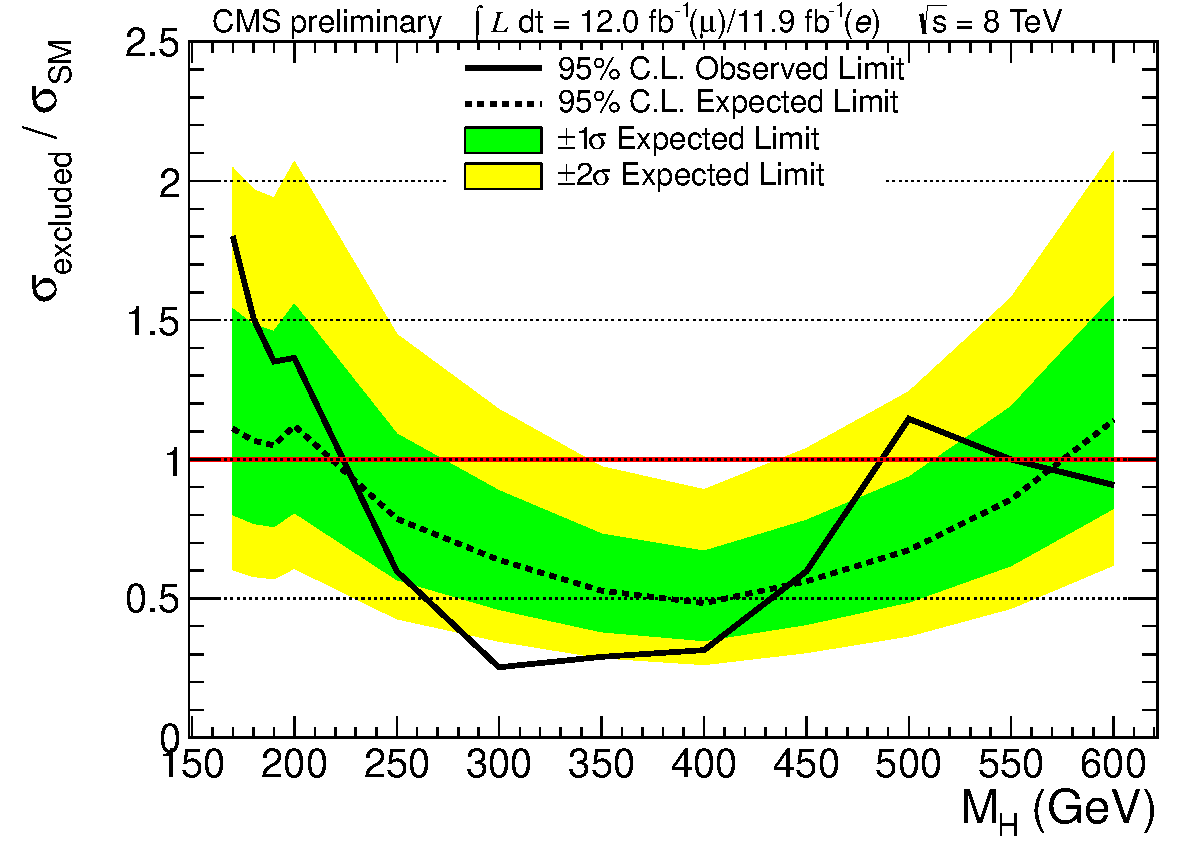
\includegraphics[width=0.49\linewidth]{plots/limit_4chan_fullsyst_asymp.pdf} % 8 TeV
    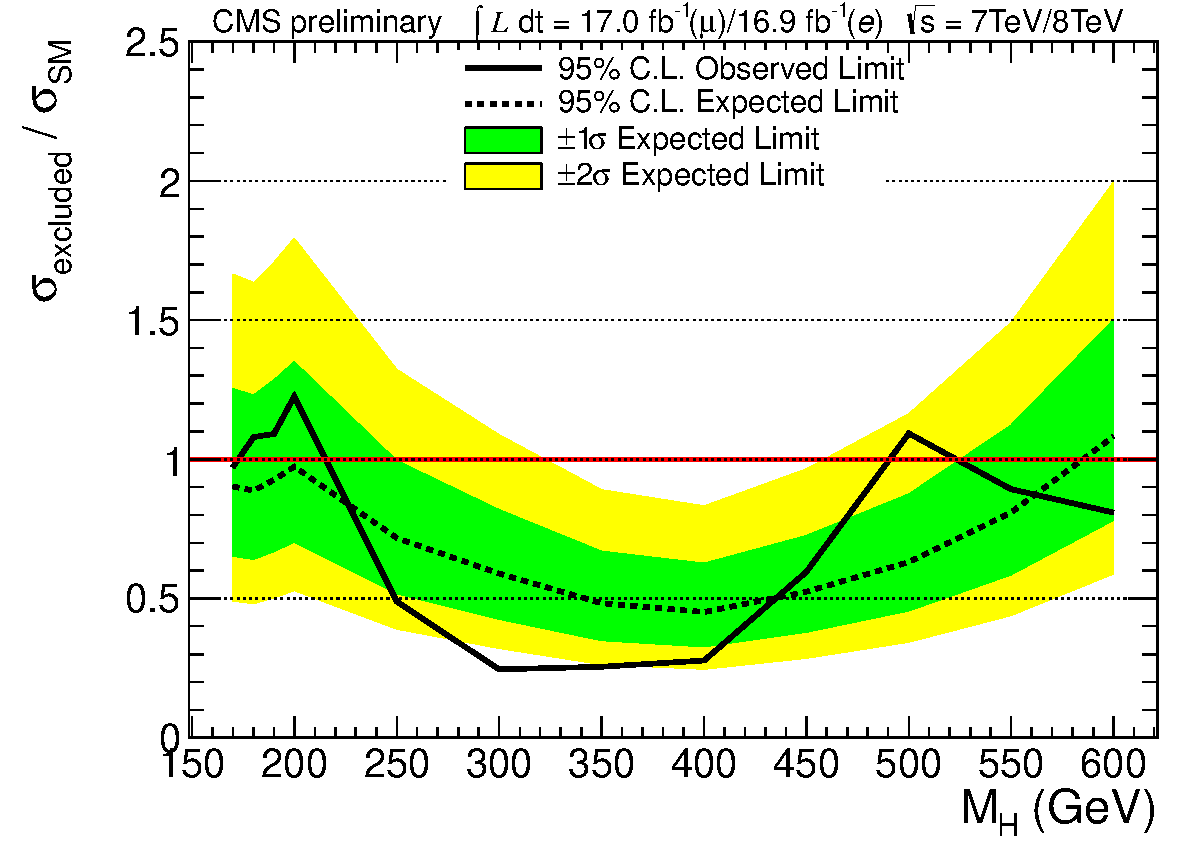
\includegraphics[width=0.49\linewidth]{plots/limit_7and8tevcombined.pdf} % 7 TeV + 8 TeV combined
    }
    \caption{Observed (solid) and expected (dashed) 95\% CL upper limit on the ratio of the
    production cross section to the SM expectation for the Higgs boson obtained using the asymptotic
    CL${}_{\textrm{S}}$ technique. The 68\% and 95\% ranges of expectation for the background-only
    model are also shown with green and yellow bands, respectively. The solid line at 1 indicates
    the SM expectation. The limit derived from 8 TeV data is shown on the left, while the combined 
    limit using both 7 TeV and 8 TeV data is shown on the right.}
    \label{fig:exclusion}
  \end{center}
\end{figure}


% ---- ---- ---- ---- ---- ---- ---- ---- ---- ---- ---- ---- ---- ---- 

\section{Conclusions}
\label{sec:summary}
A search for the SM Higgs boson decaying into two W
bosons with semi-leptonic final state has been presented 
using proton-proton collision 
data corresponding to an
integrated luminosity of 12~\fbinv
at $\sqrt{s}=8\TeV$ recorded by the CMS experiment at the LHC.  
No evidence for an additional Higgs-like boson is found  
and 95\% exclusion limits on its production cross section have been obtained.  
Using 8~TeV data, the Standard Model Higgs boson is excluded in 
the mass ranges 225--485\GeVnn and 550--600\GeVnn at 95\% confidence level,
while the median expected exclusion range is 220--560\GeVnn.
When combined with 5.0\fbinv of 7~TeV data, the exclusion ranges
expand to 215--490\GeVnn and 525--600\GeVnn at 95\% confidence level,
while the median expected one becomes 170--585\GeVnn.


% ---- ---- ---- ---- ---- ---- ---- ---- ---- ---- ---- ---- ---- ----

\section*{Acknowledgments}
% ack-text
We wish to congratulate our colleagues in the CERN accelerator departments for the excellent performance of the LHC machine. We thank the technical and administrative staff at CERN and other CMS institutes, and acknowledge support from: FMSR (Austria); FNRS and FWO (Belgium); CNPq, CAPES, FAPERJ, and FAPESP (Brazil); MES (Bulgaria); CERN; CAS, MoST, and NSFC (China); COLCIENCIAS (Colombia); MSES (Croatia); RPF (Cyprus); Academy of Sciences and NICPB (Estonia); Academy of Finland, MEC, and HIP (Finland); CEA and CNRS/IN2P3 (France); BMBF, DFG, and HGF (Germany); GSRT (Greece); OTKA and NKTH (Hungary); DAE and DST (India); IPM (Iran); SFI (Ireland); INFN (Italy); NRF and WCU (Korea); LAS (Lithuania); CINVESTAV, CONACYT, SEP, and UASLP-FAI (Mexico); MSI (New Zealand); PAEC (Pakistan); SCSR (Poland); FCT (Portugal); JINR (Armenia, Belarus, Georgia, Ukraine, Uzbekistan); MST, MAE and RFBR (Russia); MSTD (Serbia); MICINN and CPAN (Spain); Swiss Funding Agencies (Switzerland); NSC (Taipei); TUBITAK and TAEK (Turkey)
; STFC (United Kingdom); DOE and NSF (USA).
Individuals have received support from the Marie-Curie programme and the European Research Council (European Union); the Leventis Foundation; the A. P. Sloan Foundation; the Alexander von Humboldt Foundation; the Belgian Federal Science Policy Office; the Fonds pour la Formation \`a la Recherche dans l'Industrie et dans l'Agriculture (FRIA-Belgium); the Agentschap voor Innovatie door Wetenschap en Technologie (IWT-Belgium); and the Council of Science and Industrial Research, India.


%% **DO NOT REMOVE BIBLIOGRAPHY**
\bibliography{auto_generated}   % will be created by the tdr script.

